%
% $RCSfile: cybop.tex,v $
%
% Copyright (C) 2002-2008. Christian Heller.
%
% Permission is granted to copy, distribute and/or modify this document
% under the terms of the GNU Free Documentation License, Version 1.1 or
% any later version published by the Free Software Foundation; with no
% Invariant Sections, with no Front-Cover Texts and with no Back-Cover
% Texts. A copy of the license is included in the section entitled
% "GNU Free Documentation License".
%
% http://www.cybop.net
% - Cybernetics Oriented Programming -
%
% http://www.resmedicinae.org
% - Information in Medicine -
%
% Version: $Revision: 1.1 $ $Date: 2008-08-19 20:41:06 $ $Author: christian $
% Authors: Christian Heller <christian.heller@tuxtax.de>
%

%
% Determine document class specifying the type of document.
%
% Hand over font size and side format.
%
\documentclass[9pt,twoside]{tuxtax}

%
% Input hyphenation list.
%
%%
% $RCSfile: hyphenation.tex,v $
%
% Copyright (c) 2002-2007. Christian Heller. All rights reserved.
%
% Permission is granted to copy, distribute and/or modify this document
% under the terms of the GNU Free Documentation License, Version 1.1 or
% any later version published by the Free Software Foundation; with no
% Invariant Sections, with no Front-Cover Texts and with no Back-Cover
% Texts. A copy of the license is included in the section entitled
% "GNU Free Documentation License".
%
% http://www.cybop.net
% - Cybernetics Oriented Programming -
%
% Version: $Revision: 1.2 $ $Date: 2007-08-01 13:59:00 $ $Author: christian $
% Authors: Christian Heller <christian.heller@tuxtax.de>
%

\hyphenation{abs-trac-tion}
\hyphenation{ac-tu-ally}
\hyphenation{ana-lyst}
\hyphenation{ana-ly-sis}
\hyphenation{an-cient}
\hyphenation{ap-pli-ca-tion}
\hyphenation{aris-to-tle}
\hyphenation{at-tri-bute}
\hyphenation{be-ing}
\hyphenation{ca-te-go-ri-za-tion}
\hyphenation{client}
\hyphenation{com-po-nen-ti-za-tion}
\hyphenation{com-pu-ter}
\hyphenation{con-fi-gure}
\hyphenation{con-nec-ted}
\hyphenation{cy-ber-ne-tics}
\hyphenation{cyboi}
\hyphenation{cybol}
\hyphenation{cybop}
\hyphenation{des-cribed}
\hyphenation{de-sign}
\hyphenation{de-ve-lop-ment}
\hyphenation{dis-crete}
\hyphenation{di-vide}
\hyphenation{do-main}
\hyphenation{dy-na-mic}
\hyphenation{eli-mi-nate}
\hyphenation{eli-mi-nates}
\hyphenation{eli-mi-na-tion}
\hyphenation{en-gi-nee-ring}
\hyphenation{en-vi-ron-ment}
\hyphenation{ex-pert}
\hyphenation{fi-gure}
\hyphenation{fle-xi-bi-li-sie-rung}
\hyphenation{fun-da-men-tal}
\hyphenation{hard-ware}
\hyphenation{hu-man}
\hyphenation{im-ple-men-ta-tion}
\hyphenation{in-he-rit}
\hyphenation{in-he-ri-tance}
\hyphenation{in-ter-pre-ter}
\hyphenation{java}
\hyphenation{know-ledge}
\hyphenation{lan-guage}
\hyphenation{li-ving}
\hyphenation{lo-gi-cal}
\hyphenation{ma-na-ge-ment}
\hyphenation{mea-ning-ful}
\hyphenation{me-cha-nism}
\hyphenation{me-mo-ry}
\hyphenation{me-thod}
\hyphenation{me-thods}
\hyphenation{mo-del-ling}
\hyphenation{na-ture}
\hyphenation{net-work}
\hyphenation{neu-ral}
\hyphenation{neu-ron}
\hyphenation{ne-ver-en-ding-ly}
\hyphenation{open}
\hyphenation{operating}
\hyphenation{ori-en-ted}
\hyphenation{over-come}
\hyphenation{par-ti-cu-lar}
\hyphenation{prin-ci-ple}
\hyphenation{pro-ba-bi-lis-tic}
\hyphenation{pro-ble-ma-tic}
\hyphenation{pro-gram-ming}
\hyphenation{res-pon-sible}
\hyphenation{re-u-sa-bi-li-ty}
\hyphenation{sci-ence}
\hyphenation{server}
\hyphenation{si-mi-lar}
\hyphenation{soft-ware}
\hyphenation{source}
\hyphenation{spe-cia-li-za-tion}
\hyphenation{spe-ci-fied}
\hyphenation{sta-tic}
\hyphenation{sta-ti-cally}
\hyphenation{sto-chas-tic}
\hyphenation{stone-on-stone}
\hyphenation{struc-ture}
\hyphenation{strug-gling}
\hyphenation{subs-ti-tu-ting}
\hyphenation{su-per-flu-ous}
\hyphenation{sup-ply-ing}
\hyphenation{sys-tem}
\hyphenation{taeu-schungs-ver-such}
\hyphenation{temp-lates}
\hyphenation{tes-ting}
\hyphenation{thin-king}
\hyphenation{un-en-li-vened}
\hyphenation{un-sa-tis-fy-ing}
\hyphenation{va-ry-ing}
\hyphenation{weigh-ted}
\hyphenation{zu-kunfts-si-che-re}


%
% Define text macros.
%
\def\placemacro{Ilmenau}
\def\datemacro{2005-12-12}
\def\authormacro{Christian Heller}

%
% Enable special indexing commands.
% Generate contents, glossary and memo entries.
%
% Required package: makeidx
%
\makeindex

%
% This document arose from the dissertation of Christian Heller,
% written to earn a doctorate in Software Systems Engineering.
%
% Author: Christian Heller <christian.heller@tuxtax.de>
%
\begin{document}
    % Set sans serif font.
    \sffamily
    % Set page numbering to roman numbers.
    \pagenumbering{roman}
    %
% $RCSfile: cover.tex,v $
%
% Copyright (c) 2002-2007. Christian Heller. All rights reserved.
%
% Permission is granted to copy, distribute and/or modify this document
% under the terms of the GNU Free Documentation License, Version 1.1 or
% any later version published by the Free Software Foundation; with no
% Invariant Sections, with no Front-Cover Texts and with no Back-Cover
% Texts. A copy of the license is included in the section entitled
% "GNU Free Documentation License".
%
% http://www.cybop.net
% - Cybernetics Oriented Programming -
%
% Version: $Revision: 1.1 $ $Date: 2007-07-17 20:02:36 $ $Author: christian $
% Authors: Christian Heller <christian.heller@tuxtax.de>
%

%
% Defines the title page.
%
% \title and \author (and optionally \date) must be specified!
%
% Sets the page style of the first page to empty
% that is no header or footer will be shown.
%
\begin{titlepage}
    \title{
        Cybernetics Oriented Language 1.0\\
        (CYBOL)\\
        \vspace{1cm}
        % \textmd sets medium weight (default), which is the opposite of boldface.
        \normalsize{\textmd{An interpretable Knowledge Modelling- and Programming Language\\}}
    }
    \author{
        \date{
        }
    }
\end{titlepage}

    \maketitle
    % Avoid header, footer and page number.
    \thispagestyle{empty}
    \title{Flexible Software Architectures for Presentation Layers demonstrated on Medical Documentation with Episodes and Inclusion of Topological Report}
\author{Jens Bohl \(<\)info@jens-bohl.de\(>\)\\
Torsten Kunze \(<\)zone3@gmx.de\(>\)\\
Christian Heller \(<\)christian.heller@tu-ilmenau.de\(>\)\\
Ilka Philippow \(<\)ilka.philippow@tu-ilmenau.de\(>\)}
\institute{
Technical University of Ilmenau\\
Faculty for Computer Science and Automation\\
Institute for Theoretical and Technical Informatics\\
PF 100565, Max-Planck-Ring 14, 98693 Ilmenau, Germany\\
http://www.tu-ilmenau.de, fon: +49-(0)3677-69-1230, fax: +49-(0)3677-69-1220}
\maketitle

    \newpage{\pagestyle{empty}\clearpage}
    \thispagestyle{empty}
    %
% $RCSfile: copyright.tex,v $
%
% Copyright (C) 2002-2008. Christian Heller.
%
% Permission is granted to copy, distribute and/or modify this document
% under the terms of the GNU Free Documentation License, Version 1.1 or
% any later version published by the Free Software Foundation; with no
% Invariant Sections, with no Front-Cover Texts and with no Back-Cover
% Texts. A copy of the license is included in the section entitled
% "GNU Free Documentation License".
%
% http://www.cybop.net
% - Cybernetics Oriented Programming -
%
% http://www.resmedicinae.org
% - Information in Medicine -
%
% Version: $Revision: 1.1 $ $Date: 2008-08-19 20:41:06 $ $Author: christian $
% Authors: Christian Heller <christian.heller@tuxtax.de>
%

\small{Cataloging-in-Publication Data\\
    Christian Heller.\\
    Cybernetics Oriented Programming (CYBOP):\\
    An Investigation on the Applicability of Inter-Disciplinary Concepts\\
    to Software System Development\\
    Ilmenau: Tux Tax, 2006\\
    ISBN-10: 3-9810898-0-4\\
    ISBN-13: 978-3-9810898-0-6}\\

\small{Information on Ordering this book\\
    http://www.tuxtax.de, http://www.cybop.net}

\small{Written as Dissertation\\
    Supervisor 1: Prof. Dr.-Ing. habil. Ilka Philippow (Chair), Technical University of Ilmenau\\
    Supervisor 2: Prof. Dr.-Ing. habil. Dietrich Reschke, Technical University of Ilmenau, Germany\\
    Supervisor 3: Mark Lycett (PhD), Brunel University, Great Britain\\
    Submission: 2005-12-12; Presentation: 2006-10-04}

\small{Copyright \textcopyright\ 2002-2006. \authormacro. All rights reserved.}

%> \small{Translation: Christian Heller}\\ %\"Ubersetzung:
%\small{Sponsoring Editor: ??}\\ %Lektorat:
%\small{Acquisitions Editor: ??}\\
%\small{Marketing Manager: ??}\\
%\small{Marketing Assistant: ??}\\
%\small{Editorial Assistant: ??}\\
%\small{Editorial/ Production Supervision: ??}\\
%\small{Production Editor: Christian Heller}\\ %Produktion:
%\small{Production Service: ??}\\ %Produktion:
%\small{Manuscript Editor: ??}\\
%\small{Interior Illustration: ??}\\
%\small{Interior Design: ??}\\
\small{Cover Illustration: TSAMEDIEN, D\"usseldorf}\\ %Umschlaggrafik:
%\small{Cover Design: Christian Heller}\\ %Umschlaggestaltung:
%\small{Print Buyer: ??}\\
%\small{Project Coordinator: ??}\\
%> \small{Typesetting: Christian Heller, set in Times 9.5 pt font with \LaTeX\ using Kile under Linux}\\ %Satz:
%\small{Cover Printing: ??}\\
\small{Printing and Binding: Offizin Andersen Nex\"o, Leipzig/ Zwenkau} %Belichtung, Druck und Bindung:

\small{Permission is granted to copy, distribute and/or modify this document
    under the terms of the GNU Free Documentation License, Version 1.2
    or any later version published by the Free Software Foundation;
    with no Invariant Sections, with no Front-Cover Texts and with no
    Back-Cover Texts. A copy of the license is included in the section
    entitled "GNU Free Documentation License".}

\small{Trademark Credits\\
    Most of the software-, hardware- and product names used in this document
    are also trademarks or registered trademarks of their respective owners.
%    Adobe is a trademark of Adobe Systems, Incorporated.\\
%    AIX is a trademark of International Business Machines Corporation.\\
%    Arial\textregistered\ is a registered trademark of the Monotype Corporation in the United States and other countries.\\
%>    CICS is a trademark of International Business Machines Corporation.\\
%    CICS/ESA is a trademark of International Business Machines Corporation.\\
%    CorelDRAW\texttrademark\ is a trademark or registered trademark of Corel Corporation or Corel Corporation Limited.\\
%>    DB2 is a trademark of International Business Machines Corporation.\\
%    DFSMS is a trademark of International Business Machines Corporation.\\
%    DFSORT is a trademark of International Business Machines Corporation.\\
%    Energy Star\textregistered\ and the Energy Star logo\textregistered\ are registered marks of the United States Environmental Protection Agency in the United States and other countries. Details on the proper use of the marks are explained in the "Guidelines for Proper use of the Energy Star\textregistered\ Name and International Logo".\\
%>    Ethernet is a registered trademark of Xerox Corporation.\\
%>    IBM\textregistered\ is a registered trademark of International Business Machines Corporation.\\
%    IBM Warp Server\textregistered\ is a registered trademark of International Business Machines Corporation.\\
%    IMS is a trademark of International Business Machines Corporation.\\
%    IMS/ESA is a trademark of International Business Machines Corporation.\\
%>    Intel is a registered trademark of Intel Corporation in the United States and other countries.\\
%>    Java\texttrademark\ and all Java-based trademarks are trademarks of Sun Microsystems, Inc. in the United States and other countries.\\
%    Language Environment is a trademark of International Business Machines Corporation.\\
%>    Microsoft\textregistered\ is a registered trademark of Microsoft Corporation in the United States and other countries.\\
%    MS Windows\textregistered\ is a registered trademark of Microsoft Corporation in the United States and other countries.\\
%    MS-DOS\textregistered\ is a registered trademark of Microsoft Corporation in the United States and other countries.\\
%    MVS is a trademark of International Business Machines Corporation.\\
%    Netscape is a trademark of Netscape Communications Corporation in the United States and other countries.\\
%    Netscape Navigator is a trademark of Netscape Communications Corporation in the United States and other countries.\\
%    Netware\textregistered\ is a registered trademark of Novell Corporation.\\
%    Novell\textregistered\ is a registered trademark of Novell Corporation.\\
%    OpenEdition is a trademark of International Business Machines Corporation.\\
%    Opera\texttrademark\ is a trademark of Opera Software ASA.\\
%    Operating System/2\textregistered\ (OS/2) is a registered trademark of International Business Machines Corporation.\\
%    *Pantone, Inc. is a check-standard trademark for color.\\
%>    Pentium is a registered trademark of Intel Corporation in the United States and other countries.\\
%>    PostScript is a trademark of Adobe Systems, Incorporated.\\
%    RACF is a trademark of International Business Machines Corporation.\\
%    System/390 is a trademark of International Business Machines Corporation.\\
%>    Unicode is a trademark of the Unicode Consortium.\\
%>    UNIX\textregistered\ is a registered trademark of The Open Group in the United States and other countries.\\
%    VisualAge is a trademark of International Business Machines Corporation.\\
%>    Windows\textregistered\ is a registered trademark of Microsoft Corporation in the United States and other countries.\\
%    Windows NT\textregistered\ is a registered trademark of Microsoft Corporation in the United States and other countries.\\
%    z/OS is a trademark of International Business Machines Corporation.\\
%>    Other company-, product- or service names may be the trademarks or service marks of others.\\
}

\small{Donations\\
    Companies planning to publish this work on a grand scale are asked to
    notify the author \(<\)christian.heller@tuxtax.de\(>\) and to consider
    donating some of their sales revenues, which will be used exclusively for
    the CYBOP and Res Medicinae free software projects.}

\small{Text printed on recycled and acid-free paper.}

\small{Printed in Germany}

    \newpage{\pagestyle{empty}\cleardoublepage}
    % Avoid header, footer and page number.
    \thispagestyle{empty}
    %
% $RCSfile: dedication.tex,v $
%
% Copyright (c) 2002-2007. Christian Heller. All rights reserved.
%
% Permission is granted to copy, distribute and/or modify this document
% under the terms of the GNU Free Documentation License, Version 1.1 or
% any later version published by the Free Software Foundation; with no
% Invariant Sections, with no Front-Cover Texts and with no Back-Cover
% Texts. A copy of the license is included in the section entitled
% "GNU Free Documentation License".
%
% http://www.cybop.net
% - Cybernetics Oriented Programming -
%
% Version: $Revision: 1.1 $ $Date: 2007-07-17 20:02:36 $ $Author: christian $
% Authors: Christian Heller <christian.heller@tuxtax.de>
%

\vspace*{3cm}
\begin{center}
    To all Hackers (not Crackers) who stick to the ?? Hackers' Codex\\
    and contribute with great Enthusiasm to the Free Software Code Base\\
    of the Open Source Community
\end{center}

    \newpage{\pagestyle{empty}\cleardoublepage}
    \tableofcontents
    \newpage{\pagestyle{empty}\cleardoublepage}
    % Set roman font.
    \rmfamily
    %
% $RCSfile: preface.tex,v $
%
% Copyright (C) 2002-2008. Christian Heller.
%
% Permission is granted to copy, distribute and/or modify this document
% under the terms of the GNU Free Documentation License, Version 1.1 or
% any later version published by the Free Software Foundation; with no
% Invariant Sections, with no Front-Cover Texts and with no Back-Cover
% Texts. A copy of the license is included in the section entitled
% "GNU Free Documentation License".
%
% http://www.cybop.net
% - Cybernetics Oriented Programming -
%
% http://www.resmedicinae.org
% - Information in Medicine -
%
% Version: $Revision: 1.1 $ $Date: 2008-08-19 20:41:08 $ $Author: christian $
% Authors: Christian Heller <christian.heller@tuxtax.de>
%

\chapter*{Preface\markboth{Preface}{Preface}}
\label{preface_heading}
\addcontentsline{toc}{chapter}{Preface}

\begin{flushright}
    \textsl{
        I slept and dreamt that Life was Joy.\\
        I awoke and saw that Life was Service.\\
        I acted and behold, Service was joy.
    }\\
    \textsc{Rabindranath Tagore}
\end{flushright}

%
% $RCSfile: prologue.tex,v $
%
% Copyright (C) 2002-2008. Christian Heller.
%
% Permission is granted to copy, distribute and/or modify this document
% under the terms of the GNU Free Documentation License, Version 1.1 or
% any later version published by the Free Software Foundation; with no
% Invariant Sections, with no Front-Cover Texts and with no Back-Cover
% Texts. A copy of the license is included in the section entitled
% "GNU Free Documentation License".
%
% http://www.cybop.net
% - Cybernetics Oriented Programming -
%
% http://www.resmedicinae.org
% - Information in Medicine -
%
% Version: $Revision: 1.2 $ $Date: 2008-09-07 15:36:07 $ $Author: christian $
% Authors: Christian Heller <christian.heller@tuxtax.de>
%

\section*{Prologue}
\label{prologue_heading}
%\addcontentsline{toc}{section}{Prologue}

To me, basically, there are two ways to deal with a scientific subject:

\begin{enumerate}
    \item The deepened investigation on a special area aiming to find
        completely new phenomenons
    \item The systematic subsumption of multiple known aspects of one or many
        disciplines aiming to find new cross-correlations and ideas
\end{enumerate}

Both approaches may lead to new theories, methods and concepts. And both may use
laboratory trials to find and prove their theories. This work follows the second
approach. The idea behind is, simply spoken, to steal ideas from nature and
various fields of science, and to apply them to software design.

\emph{Laboratory Trials} are what \emph{Coding} is in informatics -- experiment
and proof of operability, at the same time. Some information scientists have
the opinion that coding weren't \emph{scientific} enough and not necessary to
create new theories or to achieve good results. I doubt this. In my opinion,
there are things that can only be found when actually implementing ideas in a
computer language. And in the end, a theory is worth much more when having been
proven in practice. This document contains proven ideas that were growing in my
mind over the last few years, while dealing with topics such as:

\begin{itemize}
    \item[-] Structured- and Procedural Programming
    \item[-] Object Oriented Programming
    \item[-] Design Patterns and Frameworks
    \item[-] Component Based Design and Agents
    \item[-] Ontology Structured Domain Knowledge
    \item[-] Document- and User Interface Markup
    \item[-] Persistence Mechanisms
    \item[-] System Communication
    \item[-] Operating System Concepts
\end{itemize}

The usage of typical buzzwords could not quite be avoided in this work, yet do
I hope that the ideas and results are nevertheless explained straightforward and
well enough to be really useful to some other developers out there.

This document claims to be an \emph{Academic Paper}. To all practitioners who do
not want to read it for that reason, I would like to point out that each and
every concept in it arose from practice, that is coding. Like most developers,
I started up with only a few lines of code in one Java class, later extended to
more classes, a whole framework and so on. Whenever I stumbled over difficulties,
I thought through and improved my current design by applying patterns recommended
by several software development Gurus. It was only when I realised that even
those concepts were not sufficient, that I made up my own. They are entitled
\emph{Cybernetics Oriented Programming} (CYBOP), because most ideas behind them
stem from nature.

Finally, this document has become my thesis, written to earn a doctorate
(Dr.-Ing./ PhD) in Informatics/ Software Engineering. You may wonder why I
release it under the \emph{Free Documentation License} (FDL). Well, I'm a full
supporter of the idea of \emph{Free Knowledge}, \emph{Free Software}, a
\emph{Society free of Patents} which are only hindering its development. There
are three reasons that have contributed to my decision:

\begin{enumerate}
    \item Hope to get helpful \emph{Feedback} from readers
    \item Trust in the scientific \emph{Fairness} of colleagues, worldwide, to
        properly reference this document even though it is licensed under the FDL
    \item Wish to contribute to the open source movement \emph{now} (and not in
        some years when the document might reach a more stable version), to
        speed up its successful development
\end{enumerate}

This is a growing document undergoing steady development. It is not and doesn't
claim to be free of errors nor to contain the only possible way for application
system development. So, if you find errors of whatever kind or have any helpful
ideas or constructive criticism, then please contribute them to
\(<\)christian.heller@tuxtax.de\(>\) or to the CYBOP developers mailing list
\(<\)cybop-developers@lists.berlios.de\(>\)!

%
% $RCSfile: scientific_progress.tex,v $
%
% Copyright (C) 2002-2008. Christian Heller.
%
% Permission is granted to copy, distribute and/or modify this document
% under the terms of the GNU Free Documentation License, Version 1.1 or
% any later version published by the Free Software Foundation; with no
% Invariant Sections, with no Front-Cover Texts and with no Back-Cover
% Texts. A copy of the license is included in the section entitled
% "GNU Free Documentation License".
%
% http://www.cybop.net
% - Cybernetics Oriented Programming -
%
% http://www.resmedicinae.org
% - Information in Medicine -
%
% Version: $Revision: 1.1 $ $Date: 2008-08-19 20:41:08 $ $Author: christian $
% Authors: Christian Heller <christian.heller@tuxtax.de>
%

\section*{Scientific Progress}
\label{scientific_progress_heading}
%\addcontentsline{toc}{section}{Scientific Progress}

An \emph{Abstraction} allows to capture the real world by representing it in
simplified models. Such models contain only the essential aspects of a special
domain. Any unimportant nuances, in the considered context, are neglected.
Correct abstract models is what makes science easy. Good science \emph{can} be
\emph{easy}. If it is not, then probably either:

\begin{itemize}
    \item[-] there is a \emph{mistake} in the model
    \item[-] it is not fully \emph{understood} by the scientist him/ herself
    \item[-] the explaining person wants to \emph{keep back} knowledge, making
        others look clueless
\end{itemize}

One of the biggest hindrances to scientific progress is too much or false
respect for existing solutions. No theory/ model/ concept is ever finished;
no document/ software/ product is ever fully completed. There is always room
for improvements. In the end, it is all just a person's subjective perception
and an arbitrary, abstract extract of the real world.

It is always worth reviewing and questionning everything in depth, again and
again. Standstill means regress. The best example showing how to work around
these criticisms is the \emph{Free and Open Source Software} (FOSS) movement
where all the time, existing solutions are rewritten, to be improved.

%
% $RCSfile: software_patents.tex,v $
%
% Copyright (C) 2002-2008. Christian Heller.
%
% Permission is granted to copy, distribute and/or modify this document
% under the terms of the GNU Free Documentation License, Version 1.1 or
% any later version published by the Free Software Foundation; with no
% Invariant Sections, with no Front-Cover Texts and with no Back-Cover
% Texts. A copy of the license is included in the section entitled
% "GNU Free Documentation License".
%
% http://www.cybop.net
% - Cybernetics Oriented Programming -
%
% http://www.resmedicinae.org
% - Information in Medicine -
%
% Version: $Revision: 1.1 $ $Date: 2008-08-19 20:41:08 $ $Author: christian $
% Authors: Christian Heller <christian.heller@tuxtax.de>
%

\section*{Software Patents}
\label{software_patents_heading}
%\addcontentsline{toc}{section}{Software Patents}

This work is about software. Software abstracts the real world, its items and
processes, and it can store these information and their relations which make up
actual \emph{Knowledge}. In the modern, so-called \emph{Information Society},
it becomes more and more important to have \emph{free} access to external
knowledge. This is an \emph{essential} human right and will decide about the
future living quality of people.

So much the important it is to \emph{prohibit} the application of patents to
software! They make an exclusive club of large companies own the rights on
banal, ordinary, day-to-day algorithms and methods that many people use. And,
they thereby kill any new ideas and hinder research efforts that depend on
these basic algorithms. If \emph{Software Patents} and patents on
\emph{Computer Implemented Inventions} (CII) got introduced, any free software
developer and especially \emph{Small- and Medium Sized Enterprises} (SME), the
driving force of innovation, could not unfold their full potential anymore,
since much of their time and effort would then have to go into patent inquiries
and costly legal disputes.

Software patents are dangerous for the free development of thoughts! Certain
lobbies exert an increasing influence on politics and push members of
parliaments to agitate and vote in their interest. Since probably every reader
of this document has an interest in informatics, every reader is also affected
by the software patent enforcement. But everybody can do something about it,
not only in Europe! Express your protest and sign the petition at \cite{ffii}!

%
% $RCSfile: free_publishing.tex,v $
%
% Copyright (C) 2002-2008. Christian Heller.
%
% Permission is granted to copy, distribute and/or modify this document
% under the terms of the GNU Free Documentation License, Version 1.1 or
% any later version published by the Free Software Foundation; with no
% Invariant Sections, with no Front-Cover Texts and with no Back-Cover
% Texts. A copy of the license is included in the section entitled
% "GNU Free Documentation License".
%
% http://www.cybop.net
% - Cybernetics Oriented Programming -
%
% http://www.resmedicinae.org
% - Information in Medicine -
%
% Version: $Revision: 1.1 $ $Date: 2008-08-19 20:41:06 $ $Author: christian $
% Authors: Christian Heller <christian.heller@tuxtax.de>
%

\section*{Free Publishing}
\label{free_publishing_heading}
%\addcontentsline{toc}{section}{Free Publishing}

Reputation in the scientific world strongly depends on the number of
publications in scientific journals, conference proceedings, magazines etc., of
which some have greater kudos, some less. A \emph{Philosophiae Doctor} (PhD)
student, for example, is expected to publish in some of the \emph{acknowledged}
journals, in order to be conferred a doctorate. The grant of project fundings
by local-, national- or \emph{European Union} (EU) governements and sponsorship
of a professor's department at university depend on it as well. Some unfair
practices and shortcomings of the current system of publication shall therefore
be mentioned here. There are at least four disadvantages of publishing in
scientific journals. An author:

\begin{itemize}
    \item is almost always forced to assign his copyright to the publisher;
    \item has very little chance of publishing completely new ideas, since
        evaluators (which are to guarantee a certain \emph{scientific level})
        sieve those which seem too crazy or are unknown to them and do not
        match state-of-the-art science, so that really new ideas can hardly
        become popular in this way;
    \item has to wait many months before being informed about article
        acceptance, sometimes further months to presentation at a conference
        and yet more months until a journal/ proceedings are finally available
        -- which, besides the unfine delay, is enough time for an evaluator to
        adapt the best ideas and publish them in a modified form before;
    \item and everyone else have to pay money for receiving journals (even for
        the one containing the author's own work), or become a member of
        certain scientific societies for some discount -- which means that the
        work is not freely accessible.
\end{itemize}

Further, there is something often labelled \emph{Citation Mafia}. Whether an
article gets published in a journal or not depends on it being accepted by a
number of reviewers (normally three). In order to avoid personal battles, the
article author never gets to know the evaluators' names or proficiency and has
to blindly rely on the \emph{good taste} of a conference's program committee.
However, evaluators, although tied to ethical standards, often seem to have
their list of \emph{friends} or seem to just prefer authors who have already
published elsewhere, leading to circles of scientists citing each other, quite
independent from the quality of their papers. Logically, also here, there are a
number of disadvantages:

\begin{itemize}
    \item Young scientists have a hard life and need a long time for getting
        their articles accepted, independent from how innovative they are.
    \item Mafioso scientists often warm up old stories or deliver well-formulated,
        but rubbish articles not earning the predicate \emph{scientific}.
\end{itemize}

Don't ask for proof -- I don't have it. But almost everybody in the scientific
business knows about these issues. Unfortunately, only few people \cite{jobb}
talk about- or try to change them. Obviously, many scientists prefer to either
play the same old game or are scared of personal disadvantages. However, it
feels like increasingly more researchers, in particular the new generation,
become aware that these drawbacks hinder scientific progress and new solutions
need to be found. Well, there is free online journals such as the
\emph{Journal of Free and Open Source Medical Computing} (JOSMC) \cite{josmc}
or the \emph{BioMed Central} (BMC) \cite{bmc} publisher, where research
articles are: \textit{free to access immediately, peer reviewed,
citation-tracked \ldots}

Although this document cannot deliver solutions to the above-mentioned
problems, it mentioned those to inform the reader and spur further discussion.
Supportive actions in this process would be that:

\begin{itemize}
    \item scientists acknowledge no-cost entry open source conferences like
        LinuxTag \& Co. \cite{linuxtag} as alternatives to traditional ones
    \item professors more readily accept citations of free knowledge sources
        such as Wikipedia \cite{wikipedia} in scientific works of their students
    \item students and scientists publish their works (code and documentation)
        under open source licenses
\end{itemize}

%
% $RCSfile: new_science.tex,v $
%
% Copyright (C) 2002-2008. Christian Heller.
%
% Permission is granted to copy, distribute and/or modify this document
% under the terms of the GNU Free Documentation License, Version 1.1 or
% any later version published by the Free Software Foundation; with no
% Invariant Sections, with no Front-Cover Texts and with no Back-Cover
% Texts. A copy of the license is included in the section entitled
% "GNU Free Documentation License".
%
% http://www.cybop.net
% - Cybernetics Oriented Programming -
%
% http://www.resmedicinae.org
% - Information in Medicine -
%
% Version: $Revision: 1.1 $ $Date: 2008-08-19 20:41:07 $ $Author: christian $
% Authors: Christian Heller <christian.heller@tuxtax.de>
%

\section*{New Science}
\label{new_science_heading}
%\addcontentsline{toc}{section}{New Science}

It was end of October 2004 that I discovered Stephen Wolfram's book
\emph{A New Kind of Science} \cite{wolfram} (published in 2002), through a link
in Wikipedia \cite{wikipedia}. By that time, I was already heavily writing on
my own work.

During those years of thinking about software systems, nature, the universe --
I felt pretty similar to how Wolfram describes it in the preface of his book.
Starting with an inspection of state-of-the-art techniques, diving deeper and
deeper into several topics, I soon realised that they all could not deliver a
\emph{coherent}, \emph{conclusive} solution to software modelling. Each had its
own drawbacks that made workarounds necessary. And, the more I dived into the
different technologies, the more complex, complicated, intransparent they got
-- but still, none seemed to provide an \emph{overall} solution.

It was only when I got more and more distance to existing solutions and moved
away from current thinking, towards a more universal approach and a view at
software systems through the eyes of nature, that I found the basic principles
described in this work.

Now, after having read \emph{A New Kind of Science}, I am glad that Wolfram did
not already write down everything I want to say, so that there is something left
for me to contribute, by delivering this work :-) There is one difference that
soon became obvious to me: Wolfram argues, that it is possible to study the
abstract world of simple programs, and take lessons from what kinds of things
occur there and have them in mind when investigating natural systems
\cite{wikipedia}. My work follows the exact opposite way, in that it observes
phenomenons of nature and concepts used in other sciences, and tries to apply
them to the design of software systems.

This is \emph{not} to say that \emph{CYBOP} does provide \emph{the} overall
solution. But what it surely wants to reach is to encourage people to think in
more general terms, across disciplines, to possibly find new concepts. And for
that, this work hopes to deliver some ideas. And I certainly do hope that the
more you, as readers, think about these ideas, the more sense they will make to
you, too.

%
% $RCSfile: stylistic_means.tex,v $
%
% Copyright (c) 2002-2007. Christian Heller. All rights reserved.
%
% Permission is granted to copy, distribute and/or modify this document
% under the terms of the GNU Free Documentation License, Version 1.1 or
% any later version published by the Free Software Foundation; with no
% Invariant Sections, with no Front-Cover Texts and with no Back-Cover
% Texts. A copy of the license is included in the section entitled
% "GNU Free Documentation License".
%
% http://www.cybop.net
% - Cybernetics Oriented Programming -
%
% Version: $Revision: 1.1 $ $Date: 2007-07-17 20:02:36 $ $Author: christian $
% Authors: Christian Heller <christian.heller@tuxtax.de>
%

\section*{Stylistic Means and Notation}
\label{stylistic_means_heading}
%\addcontentsline{toc}{section}{Stylistic Means and Notation}

The language of choice in this document is \emph{British English}, more
precisely known as \emph{Commonwealth English}. Exceptions are citations or
proper names like \emph{Unified Modeling Language}, stemming from
\emph{American English} sources. (In Oxford English, \emph{Modelling} would be
written with double letter \emph{l}). I am thinking about writing a
\emph{German} version of this document, but am not sure if it will be worth the
effort. If you as reader are interested in a translation, send me a short note!
The more emails I receive, the more convinced I will be.

% Als Autor dieser Arbeit konnte ich mir die Freiheit nehmen, viele Textpassagen
% nicht wortgetreu, sondern vielmehr sinngem�� aus der englischen Originalfassung
% zu �bersetzen. Fachbegriffe aus der Computerwelt wurden in Englisch belassen,
% um keine Zweideutigkeiten und redundante Abk�rzungen entstehen zu lassen.

Correctly, masculine \emph{and} feminine forms are used in a work. When
describing a patient's record, for example, one would write: \textit{his or her
record}. In order to improve readability, and exclusively because of this
reason, only masculine forms are used in this work.

Pieces of software source code are displayed in \texttt{Typewriter Typeface}.
Emphasised words are \emph{italicised}.

Footnotes are not used on purpose. In my opinion, they only interrupt the
flow-of-reading. Remarks are placed in context instead, sometimes enclosed in
parentheses.

%
% $RCSfile: acknowledgements.tex,v $
%
% Copyright (C) 2002-2008. Christian Heller.
%
% Permission is granted to copy, distribute and/or modify this document
% under the terms of the GNU Free Documentation License, Version 1.1 or
% any later version published by the Free Software Foundation; with no
% Invariant Sections, with no Front-Cover Texts and with no Back-Cover
% Texts. A copy of the license is included in the section entitled
% "GNU Free Documentation License".
%
% http://www.cybop.net
% - Cybernetics Oriented Programming -
%
% http://www.resmedicinae.org
% - Information in Medicine -
%
% Version: $Revision: 1.1 $ $Date: 2008-08-19 20:41:05 $ $Author: christian $
% Authors: Christian Heller <christian.heller@tuxtax.de>
%

\section*{Acknowledgements}
\label{acknowledgements_heading}
%\addcontentsline{toc}{section}{Acknowledgements}

Certainly, first thanks is due my wife \emph{Kasia} and my \emph{Parents} and
\emph{Sisters}, being always with me, in good as in bad times. Not less
important to me are my aunt \emph{Maria Kosiza}, my great \emph{Relatives} and
our former chaplain \emph{Johannes Preis}, who have helped shaping me the way I
am.

I would like to thank my professor, \emph{Ilka Philippow}, for greatly
encouraging me during my work while leaving enough room to develop my own
ideas. Equal thanks is due my supervisors \emph{Dietrich Reschke} and
\emph{Mark Lycett}. \emph{Detlef Streitferdt} and \emph{Bernd D\"ane} gave
numerous hints improving the quality of the first part of my work. Consultation
with Bernd and \emph{Wolfgang Fengler} helped me understand Petri Net diagrams
and their hardware background as well as Assembler programming. Whenever I
got doubts about what I was doing, I was very lucky to receive good motivation
from my colleagues \emph{Volker Langenhan}, \emph{Oswald Kowalski},
\emph{Todor Vangelov} and \emph{Kai B\"ollert}. Oswald's talks about hardware
concepts made me find useful parallels to software. Alexander Fleischer helped
out when I was struggling with \LaTeX's paper size option.

My thanks go to my students \emph{Jens Bohl}, \emph{Torsten Kunze},
\emph{Dirk Behrendt}, \emph{Kumanan Kanagasabapathy}, \emph{Jens Kleinschmidt},
\emph{Martin Fache}, \emph{Karsten Tellhelm}, \emph{Marcel Kiesling},
\emph{Teodora Kikova}, \emph{Dennis Reichenbach}, \emph{Stefan Zeisler},
\emph{Michael Simon}, \emph{Henrik Brandes} and \emph{Saddia Malik} for
contributing their theses, tutorials or source code to the project. Special
thanks to \emph{Rolf Holzm\"uller} who brought in some innovative ideas for
CYBOL, in the final phase of my work, and helped cleaning many bugs in CYBOI.

Reminiscences on good times go to my former colleagues of \emph{OWiS Software}
who, together with the \emph{Technical University of Ilmenau} (TUI), have
contributed with great commitment to the development of the
\emph{Object Technology Workbench} (OTW) UML tool which I would have liked to
use in the early stages of my work. Pity it hasn't gone Open Source after its
development was stopped in 2000 :-( Thanks to \emph{Martin Wolf},
\emph{Rene Prei\ss{}el}, \emph{Dirk Henning} and all colleagues who have been
patient and well-explaining teachers!

I would like to acknowledge the contributors of \emph{CYBOP} \cite{cybop} and
\emph{Res Medicinae} \cite{resmedicinae}, especially all medical doctors, e.g.
\emph{Claudia Neumann} and \emph{Karsten Hilbert}, who supported the second
project with their analysis work \cite{resmedicinae2001} and mailing list
discussions. Furthermore, I want to mention \emph{Thomas Beale} from the
\emph{OpenEHR} project \cite{openehr} whose freely published design document
(back in 2001) gave me some initial ideas in the early stage of my work.
Acknowledged be all these brave \emph{Enthusiasts} of the
\emph{Free/ Libre Open Source Software} (FLOSS) community, who have provided me
with a great amount of knowledge through a comprising code base to build on.
I shall mention the contributors of FLOSS projects such as \emph{Scope}
\cite{scope}, \emph{Apache Jakarta} \cite{jakarta}, \emph{JOS} \cite{jos},
\emph{JDistro} \cite{jdistro}, the \emph{OpenHealth} \cite{openhealth} mailing
list readers, the \emph{OSHCA} \cite{oshca} members and all other supporters of
our projects and ideals.

Great thanks goes to the \emph{Urban und Fischer} publishing company, for
providing anatomical images from their \emph{Sobotta: Atlas der Anatomie}
\cite{urban} and to the \emph{Open Clip Art} project \cite{openclipart} for its
wonderful library of free art! Similarly, I have to thank the free online
dictionaries of \emph{LEO} \cite{leo} and the
\emph{Technical University of Chemnitz} \cite{tuchemnitz}.

I am grateful to all people who openly publish their knowledge on the web.
Without the numerous free sources, I would have never been able to accomplish
this work. Especially in the state-of-the-art part, I had to heavily rely on
existing sources. It is also therefore that I have decided to put my work under
the \emph{GNU FDL} licence \cite{gnulicences}. I would be happy to see large
parts of it copied in \emph{Wikipedia} \cite{wikipedia}!


Let me finish this preface with \textsc{Arthur Schopenhauer}'s words:

\begin{flushright}
    \textsl{
        All truth passes through three stages:\\
        First, it is ridiculed.\\
        Second, it is violently opposed.\\
        Third, it is accepted as being self-evident.
    }\\
\end{flushright}

Thank you for reading!

\vspace{1cm}

\textit{
    \placemacro,
    October 2006
    \hfill{\authormacro}
    \(<\)christian.heller@tuxtax.de\(>\)
}

\vfill

    \newpage{\pagestyle{empty}\cleardoublepage}
    % Set page numbering to arabic numbers.
    \pagenumbering{arabic}
    %
% $RCSfile: introduction.tex,v $
%
% Copyright (c) 2002-2007. Christian Heller. All rights reserved.
%
% Permission is granted to copy, distribute and/or modify this document
% under the terms of the GNU Free Documentation License, Version 1.1 or
% any later version published by the Free Software Foundation; with no
% Invariant Sections, with no Front-Cover Texts and with no Back-Cover
% Texts. A copy of the license is included in the section entitled
% "GNU Free Documentation License".
%
% http://www.cybop.net
% - Cybernetics Oriented Programming -
%
% Version: $Revision: 1.1 $ $Date: 2007-07-17 20:02:36 $ $Author: christian $
% Authors: Christian Heller <christian.heller@tuxtax.de>
%

\chapter{Introduction}
\label{introduction_heading}
\index{Introduction}

This is just a test \cite{zimmermann} citation.

%
% $RCSfile: terminology.tex,v $
%
% Copyright (C) 2002-2008. Christian Heller.
%
% Permission is granted to copy, distribute and/or modify this document
% under the terms of the GNU Free Documentation License, Version 1.1 or
% any later version published by the Free Software Foundation; with no
% Invariant Sections, with no Front-Cover Texts and with no Back-Cover
% Texts. A copy of the license is included in the section entitled
% "GNU Free Documentation License".
%
% http://www.cybop.net
% - Cybernetics Oriented Programming -
%
% http://www.resmedicinae.org
% - Information in Medicine -
%
% Version: $Revision: 1.1 $ $Date: 2008-08-19 20:41:09 $ $Author: christian $
% Authors: Christian Heller <christian.heller@tuxtax.de>
%

\subsection{Terminology}
\label{terminology_heading}
\index{Terminology}
\index{Lexicon}
\index{Vocabulary}
\index{Nomenclature}
\index{Hierarchy}
\index{Semantic Link}
\index{Directed Acyclic Graph}
\index{DAG}

While a \emph{Lexicon} is a list of pure words, a \emph{Terminology} (sometimes
called \emph{Vocabulary}) can also contain phrases. Because it is a fixed list
of lots of terms, a terminology should exclude any link to a separate list of
concepts. When a terminology contains additional instructions describing how to
interpret each term, or dictating when to choose one over another
(prioritisation), it may be called a \emph{Nomenclature}. The knowledge schema
proposed in this work (chapter \ref{knowledge_schema_heading}) shall be capable
of storing codes of various terminology systems.

Lexicon and terminology stand for a \emph{Set} of words or terms, respectively.
To bring some structure into such a set, terms or concepts need to be ordered,
that is organised through a system of links, into a \emph{Hierarchy}, which
Rogers \cite{rogers} defines as a:

\begin{quote}
    \ldots\ tree-like structure, where things at the top of the tree are in some
    way more general or abstract than the things lower down. The nature of each
    link between each level in the tree may be explicit or only implied, and
    more than one flavour of semantic link can be used to build the tree (in
    which case it may be called a \emph{Mixed Hierarchy}).
\end{quote}

Kinds of hierarchies, as means of organisation, are:

\begin{itemize}
    \item[-] \emph{Subsumption Hierarchy} (Classification, Taxonomy): only
        \emph{is-a} relationships exist between parent-child pairs in the tree
    \item[-] \emph{Uniaxial Hierarchy:} each concept only ever has one parent,
        though it can have more than one child
    \item[-] \emph{Multiaxial Hierachy:} each concept can have more than one
        parent as well as more than one child
    \item[-] \emph{Exhaustive Multiaxial Hierarchy:} all concepts have all the
        parents as well as all the children they should have
\end{itemize}

As organisation \emph{Rules} count:

\begin{itemize}
    \item[-] \emph{Formalism}: an explicitly expressed set of rules, like the
        specification for how to tell what should (not) be a parent of a concept
    \item[-] \emph{Concept System} (Model): a system of \emph{Symbols} that
        stand in for concepts and/ or the links between them, and which may or
        may not be intended to be processed with reference to some formalism
    \item[-] \emph{Partonomy} (Mereology): a system of concepts and links
        intended to represent whole-part relationships specifically
\end{itemize}

On a yet higher abstract level, a \emph{Data Structure} may hold organisations
of concepts. Various types of data structures are:

\begin{itemize}
    \item[-] \emph{Network}: a mesh-like structure that connects terms or concepts
        using links; a hierarchy can be thought of as simple case of a network
    \item[-] \emph{Graph}: a network
    \item[-] \emph{Directed Graph}: a network in which each link has a \emph{Direction}
    \item[-] \emph{Directed Acyclic Graph} (DAG): a directed graph free of loops
\end{itemize}

A knowledge template expressed in the language that will be defined in chapter
\ref{cybernetics_oriented_language_heading} describes an uniaxial hierarchy,
that is its sub concepts have just one parent node. Its structure follows the
partonomy (mereology) organisation rules and represents a DAG.

%
% $RCSfile: cybernetics_oriented_programming.tex,v $
%
% Copyright (c) 2002-2007. Christian Heller. All rights reserved.
%
% Permission is granted to copy, distribute and/or modify this document
% under the terms of the GNU Free Documentation License, Version 1.1 or
% any later version published by the Free Software Foundation; with no
% Invariant Sections, with no Front-Cover Texts and with no Back-Cover
% Texts. A copy of the license is included in the section entitled
% "GNU Free Documentation License".
%
% http://www.cybop.net
% - Cybernetics Oriented Programming -
%
% Version: $Revision: 1.1 $ $Date: 2007-07-17 20:02:36 $ $Author: christian $
% Authors: Christian Heller <christian.heller@tuxtax.de>
%

\section{Cybernetics Oriented Programming}
\label{cybernetics_oriented_programming_heading}
\index{Cybernetics Oriented Programming}

The \emph{Cybernetics Oriented Programming} (CYBOP) software development theory
suggests to ...

%
% $RCSfile: software_engineering_process.tex,v $
%
% Copyright (c) 2002-2007. Christian Heller. All rights reserved.
%
% Permission is granted to copy, distribute and/or modify this document
% under the terms of the GNU Free Documentation License, Version 1.1 or
% any later version published by the Free Software Foundation; with no
% Invariant Sections, with no Front-Cover Texts and with no Back-Cover
% Texts. A copy of the license is included in the section entitled
% "GNU Free Documentation License".
%
% http://www.cybop.net
% - Cybernetics Oriented Programming -
%
% Version: $Revision: 1.1 $ $Date: 2007-07-17 20:02:36 $ $Author: christian $
% Authors: Christian Heller <christian.heller@tuxtax.de>
%

\subsection{Software Engineering Process}
\label{software_engineering_process_heading}
\index{Software Engineering Process}

Although hundreds of variations, with or without iterations, exist, a standard
\emph{Software Engineering Process} (SEP) consists of the phases: \emph{Analysis},
\emph{Design} and \emph{Implementation}, as illustrated in figure
\ref{software_engineering_process_figure}.

\begin{figure}[ht]
    \begin{center}
        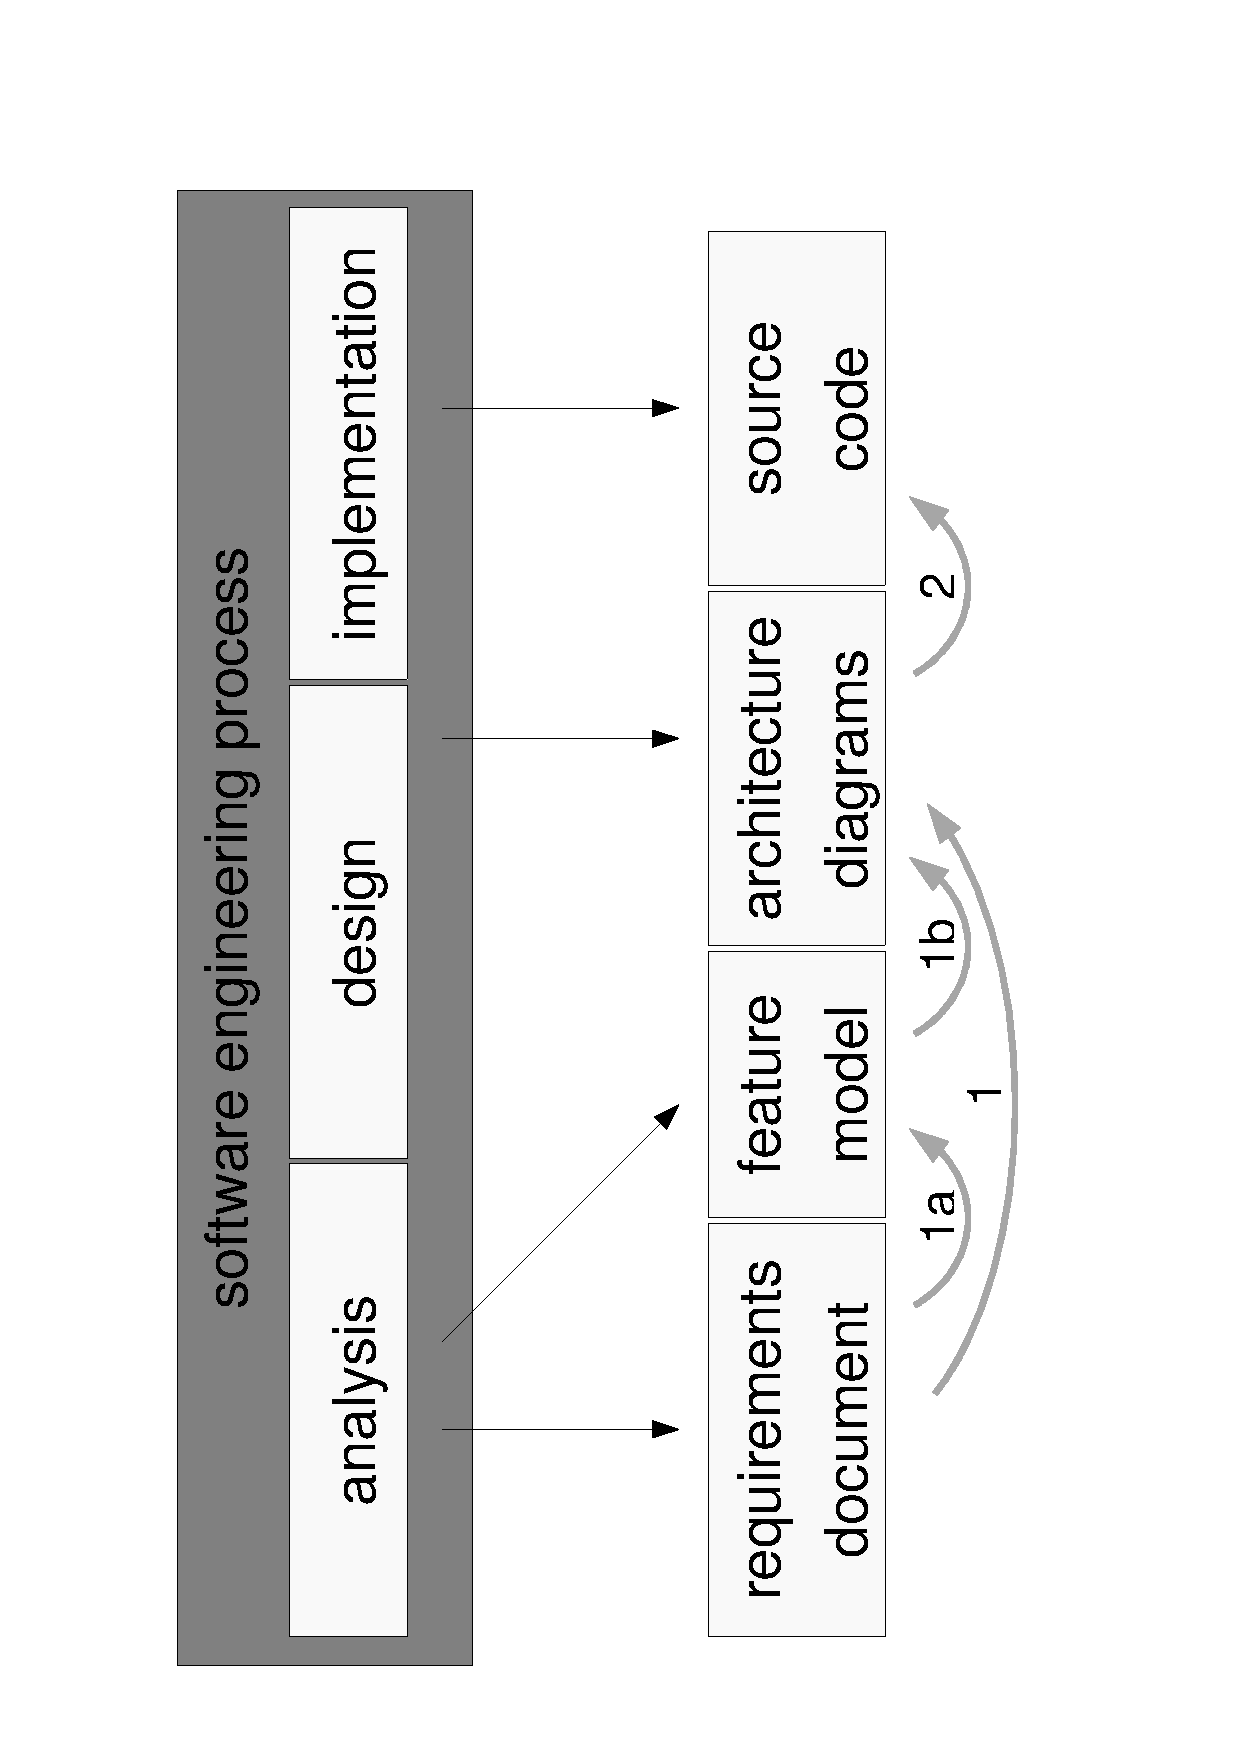
\includegraphics[scale=0.3,angle=-90]{graphics/gaps.pdf}
        \caption{Standard Software Engineering Process}
        \label{software_engineering_process_figure}
    \end{center}
\end{figure}

%
% $RCSfile: interpretation.tex,v $
%
% Copyright (c) 2002-2007. Christian Heller. All rights reserved.
%
% Permission is granted to copy, distribute and/or modify this document
% under the terms of the GNU Free Documentation License, Version 1.1 or
% any later version published by the Free Software Foundation; with no
% Invariant Sections, with no Front-Cover Texts and with no Back-Cover
% Texts. A copy of the license is included in the section entitled
% "GNU Free Documentation License".
%
% http://www.cybop.net
% - Cybernetics Oriented Programming -
%
% Version: $Revision: 1.1 $ $Date: 2007-07-17 20:02:36 $ $Author: christian $
% Authors: Christian Heller <christian.heller@tuxtax.de>
%

\subsection{Interpretation}
\label{inerpretation_heading}
\index{Interpretation}

CYBOP
CYBOL
CYBOI

\begin{figure}[ht]
    \begin{center}
        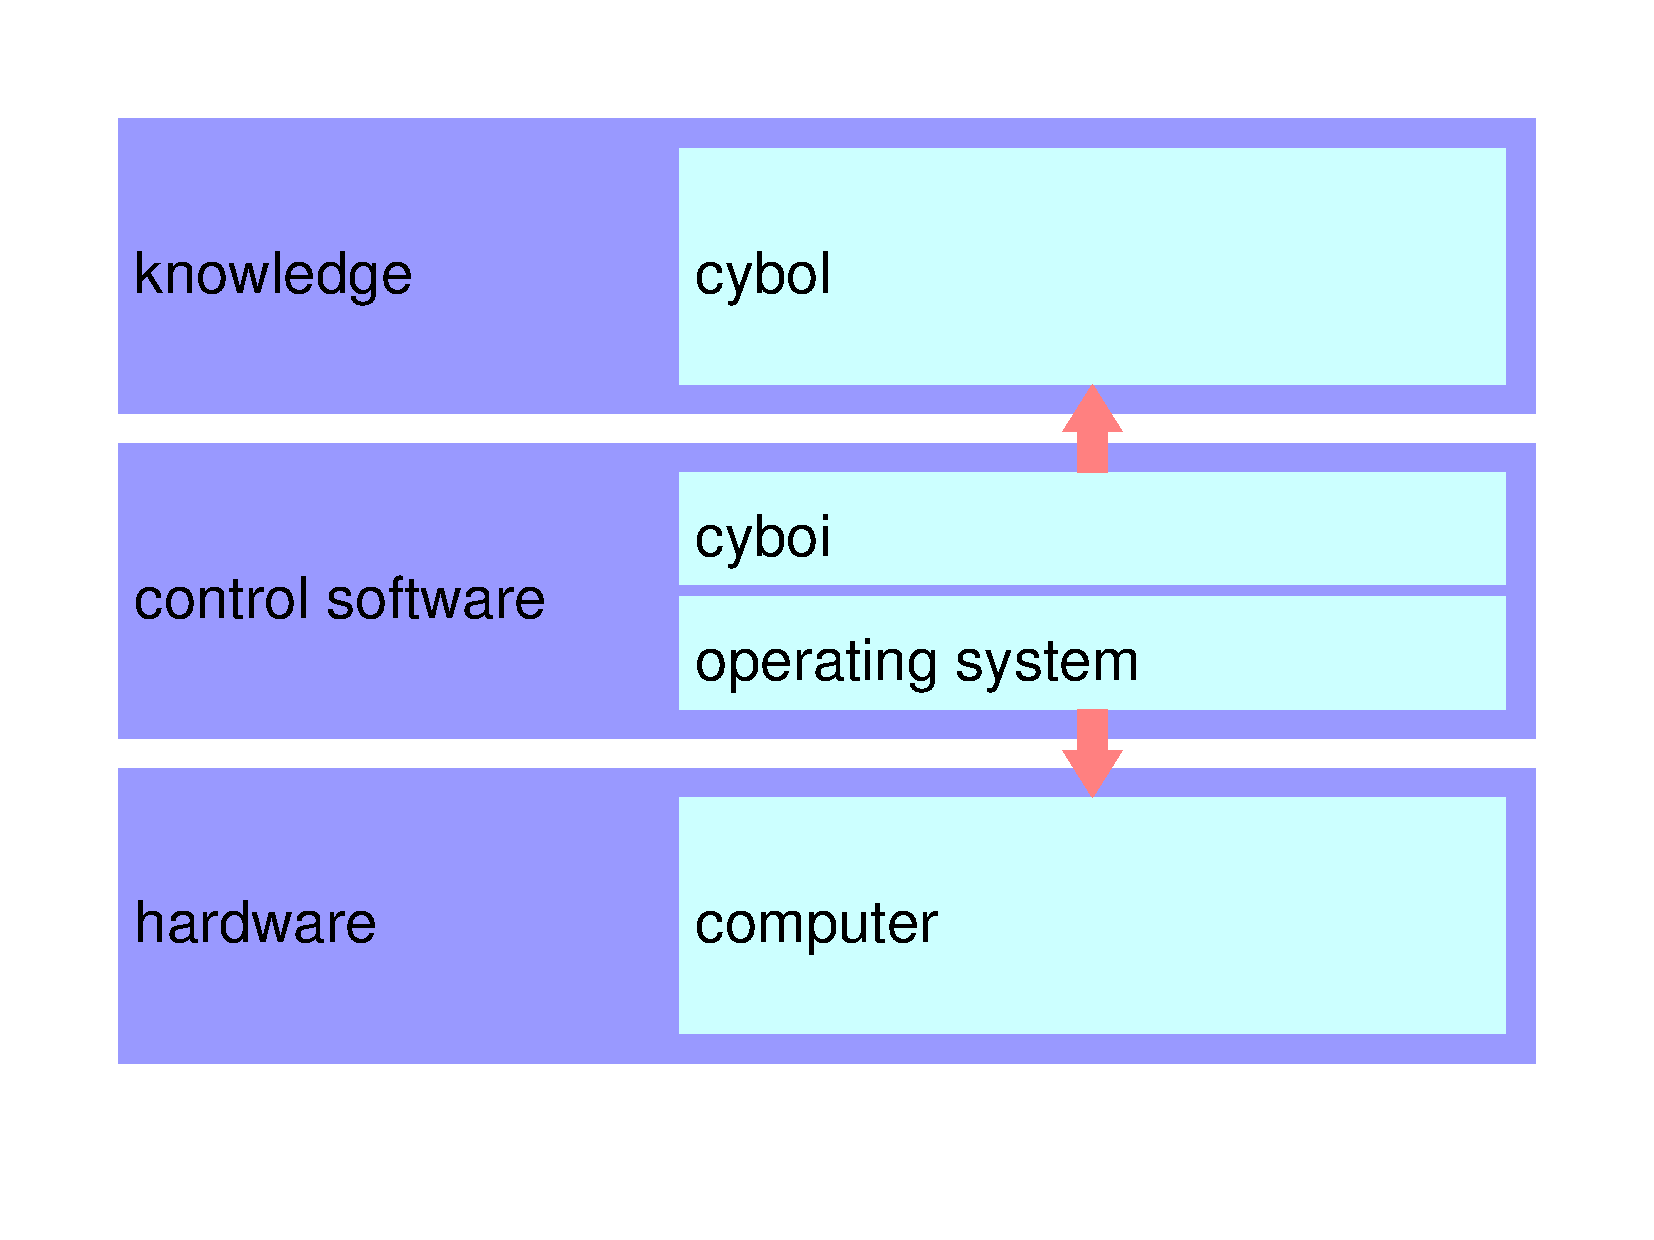
\includegraphics[scale=0.3,angle=-90]{graphics/connection.pdf}
        \caption{CYBOL Interpretation}
        \label{cybol_interpretation_figure}
    \end{center}
\end{figure}


%
% $RCSfile: extensible_markup_language.tex,v $
%
% Copyright (c) 2002-2007. Christian Heller. All rights reserved.
%
% Permission is granted to copy, distribute and/or modify this document
% under the terms of the GNU Free Documentation License, Version 1.1 or
% any later version published by the Free Software Foundation; with no
% Invariant Sections, with no Front-Cover Texts and with no Back-Cover
% Texts. A copy of the license is included in the section entitled
% "GNU Free Documentation License".
%
% http://www.cybop.net
% - Cybernetics Oriented Programming -
%
% Version: $Revision: 1.1 $ $Date: 2007-07-17 20:02:36 $ $Author: christian $
% Authors: Christian Heller <christian.heller@tuxtax.de>
%

\section{Extensible Markup Language}
\label{extensible_markup_language_heading}
\index{Extensible Markup Language}

The \emph{Extensible Markup Language} (XML) is ...


    \newpage{\pagestyle{empty}\cleardoublepage}
    %
% $RCSfile: basics.tex,v $
%
% Copyright (C) 2002-2008. Christian Heller.
%
% Permission is granted to copy, distribute and/or modify this document
% under the terms of the GNU Free Documentation License, Version 1.1 or
% any later version published by the Free Software Foundation; with no
% Invariant Sections, with no Front-Cover Texts and with no Back-Cover
% Texts. A copy of the license is included in the section entitled
% "GNU Free Documentation License".
%
% http://www.cybop.net
% - Cybernetics Oriented Programming -
%
% http://www.resmedicinae.org
% - Information in Medicine -
%
% Version: $Revision: 1.1 $ $Date: 2008-08-19 20:41:05 $ $Author: christian $
% Authors: Christian Heller <christian.heller@tuxtax.de>
%

\part{Basics}
\label{basics_heading}
\newpage{\pagestyle{empty}\cleardoublepage}

%
% $RCSfile: software_engineering_process.tex,v $
%
% Copyright (c) 2002-2007. Christian Heller. All rights reserved.
%
% Permission is granted to copy, distribute and/or modify this document
% under the terms of the GNU Free Documentation License, Version 1.1 or
% any later version published by the Free Software Foundation; with no
% Invariant Sections, with no Front-Cover Texts and with no Back-Cover
% Texts. A copy of the license is included in the section entitled
% "GNU Free Documentation License".
%
% http://www.cybop.net
% - Cybernetics Oriented Programming -
%
% Version: $Revision: 1.1 $ $Date: 2007-07-17 20:02:36 $ $Author: christian $
% Authors: Christian Heller <christian.heller@tuxtax.de>
%

\subsection{Software Engineering Process}
\label{software_engineering_process_heading}
\index{Software Engineering Process}

Although hundreds of variations, with or without iterations, exist, a standard
\emph{Software Engineering Process} (SEP) consists of the phases: \emph{Analysis},
\emph{Design} and \emph{Implementation}, as illustrated in figure
\ref{software_engineering_process_figure}.

\begin{figure}[ht]
    \begin{center}
        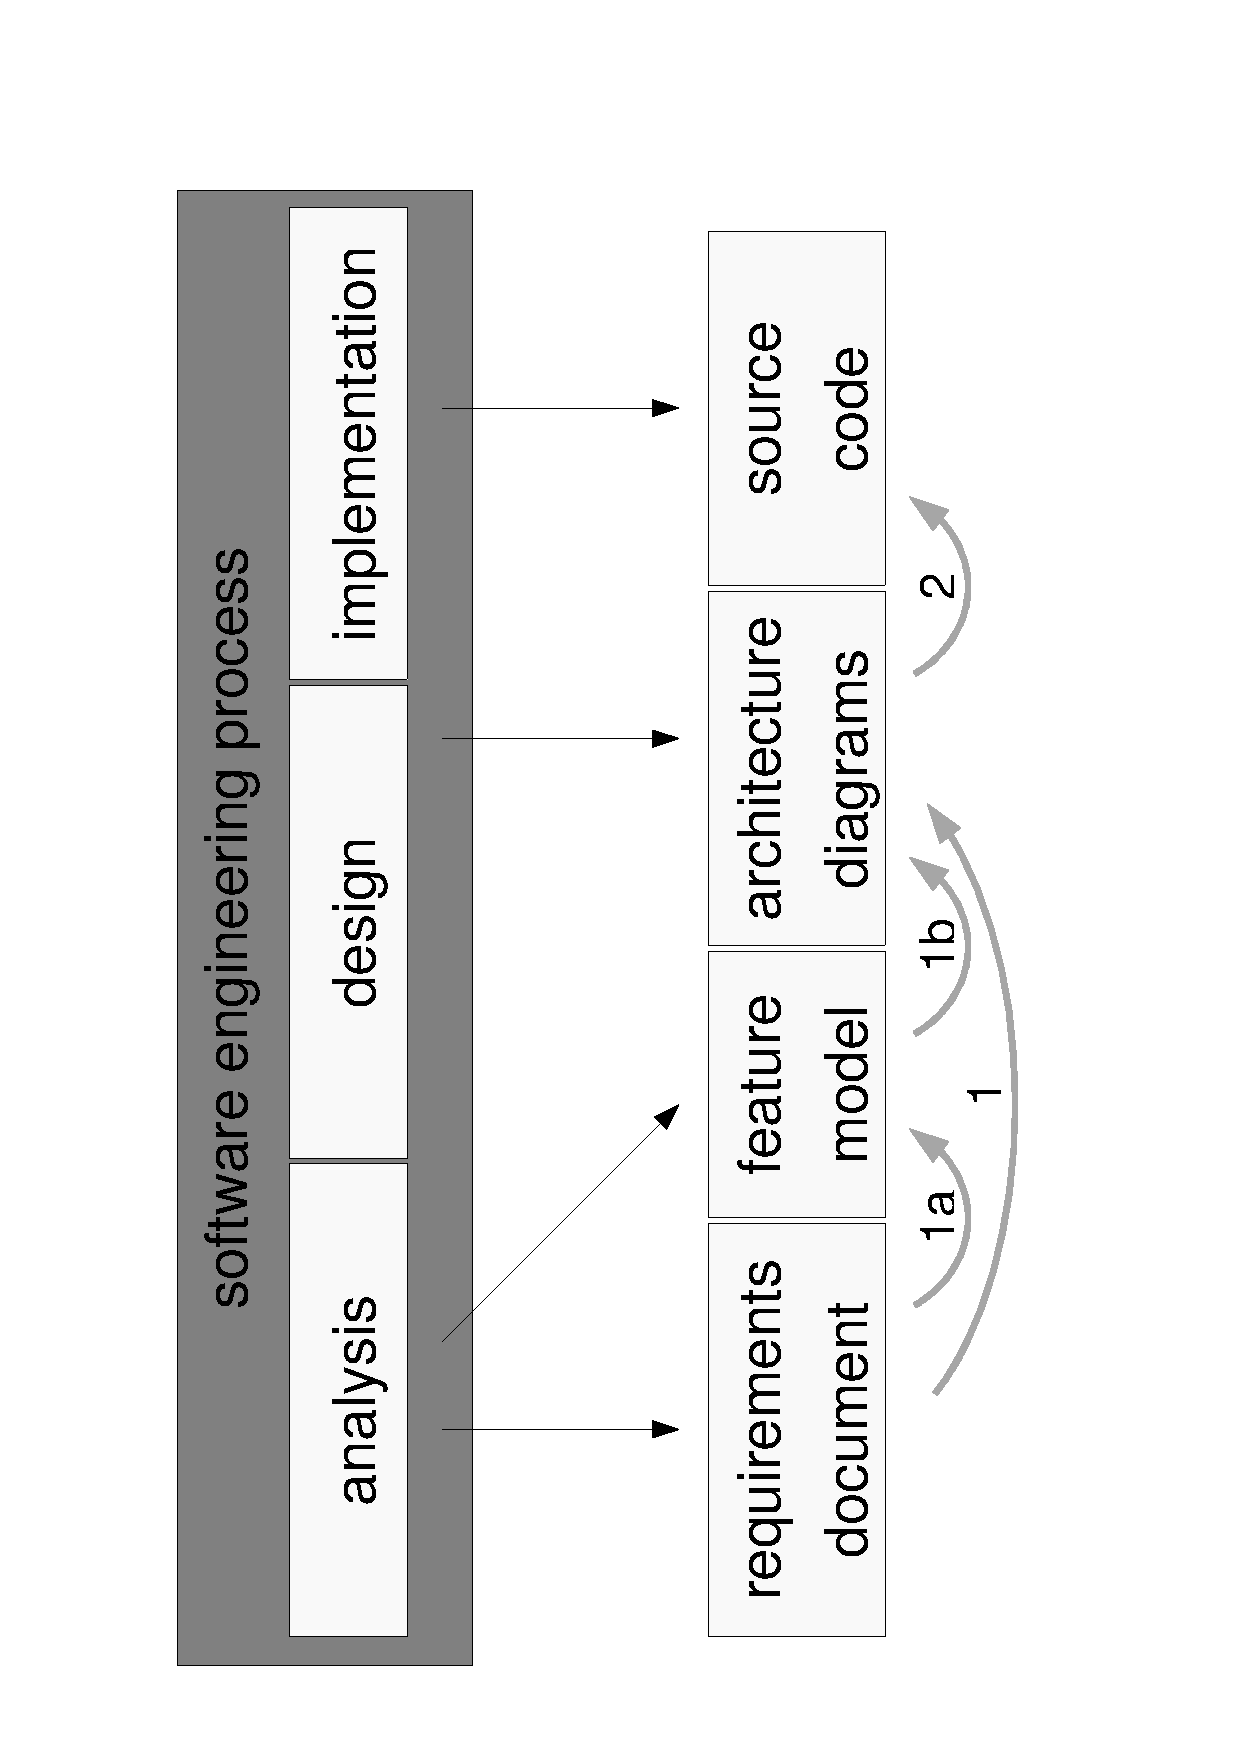
\includegraphics[scale=0.3,angle=-90]{graphics/gaps.pdf}
        \caption{Standard Software Engineering Process}
        \label{software_engineering_process_figure}
    \end{center}
\end{figure}

\newpage{\pagestyle{empty}\cleardoublepage}
%
% $RCSfile: physical_architecture.tex,v $
%
% Copyright (C) 2002-2008. Christian Heller.
%
% Permission is granted to copy, distribute and/or modify this document
% under the terms of the GNU Free Documentation License, Version 1.1 or
% any later version published by the Free Software Foundation; with no
% Invariant Sections, with no Front-Cover Texts and with no Back-Cover
% Texts. A copy of the license is included in the section entitled
% "GNU Free Documentation License".
%
% http://www.cybop.net
% - Cybernetics Oriented Programming -
%
% http://www.resmedicinae.org
% - Information in Medicine -
%
% Version: $Revision: 1.1 $ $Date: 2008-08-19 20:41:08 $ $Author: christian $
% Authors: Christian Heller <christian.heller@tuxtax.de>
%

\chapter{Physical Architecture}
\label{physical_architecture_heading}
\index{Physical Architecture}
\index{Communication}
\index{Autonomous Systems}
\index{Interaction and Cooperation}
\index{Technical Systems}
\index{Computer}
\index{Client}
\index{Server}
\index{Communication Partners}
\index{System Constellations}
\index{Communication Languages}
\index{Information Technology Environment}
\index{IT}

\begin{flushright}
    \textsl{Simplicity is the Result of Maturity.}\\
    \textsc{Johann Christoph Friedrich von Schiller}
\end{flushright}

Software provides the functionality through which robots act and computers
represent and process information. Both are special kinds of machines which only
get useful for humans if they can be controlled and communicated with.
\emph{Communication} is an essential ability for almost any kind of system.
\emph{Autonomous} systems exist and may well be useful, but is it nearly always
the \emph{Interaction} and \emph{Cooperation} that makes technical systems (from
now on called \emph{Computer} in this work) so interesting and helpful to humans.

In many cases, systems are limited to one role: \emph{Client} or \emph{Server}.
Clients ask questions which servers answer. But both are able to send as well
as to receive information. One-way communication without any feedback is rarely
useful. Besides the mentioned client- and server-, there are other roles that a
computer system can take on when talking with so-called
\emph{Communication Partners}.

The following sections will stepwise build up- and briefly investigate some
examples of well-known system constellations and possible communication
languages that are commonly used in a general \emph{Information Technology}
(IT) environment. Because physical systems and their interactions are
considered without any knowledge about their inside, one also talks of this as
the \emph{Physical Architecture} of an IT environment. Its understanding is
important for later reflections on the inner architecture of software systems
(chapter \ref{logical_architecture_heading}). Also will chapter
\ref{state_and_logic_heading} come back to system communication principles and
introduce a translator architecture for universal communication.

%
% $RCSfile: process.tex,v $
%
% Copyright (C) 2002-2008. Christian Heller.
%
% Permission is granted to copy, distribute and/or modify this document
% under the terms of the GNU Free Documentation License, Version 1.1 or
% any later version published by the Free Software Foundation; with no
% Invariant Sections, with no Front-Cover Texts and with no Back-Cover
% Texts. A copy of the license is included in the section entitled
% "GNU Free Documentation License".
%
% http://www.cybop.net
% - Cybernetics Oriented Programming -
%
% http://www.resmedicinae.org
% - Information in Medicine -
%
% Version: $Revision: 1.1 $ $Date: 2008-08-19 20:41:08 $ $Author: christian $
% Authors: Christian Heller <christian.heller@tuxtax.de>
%

\section{Process}
\label{process_heading}
\index{Process}
\index{Resource Grouping}
\index{Execution}
\index{Address Space}
\index{Thread of Execution}
\index{Central Processing Unit}
\index{CPU}
\index{Program Counter}
\index{Registers}
\index{Stack}
\index{Abstract System Concepts}
\index{Operating System}
\index{OS}
\index{Session}
\index{Process Group}
\index{Job}
\index{System}
\index{Application}
\index{Task}
\index{Lightweight Process}
\index{Work Queue}
\index{Task Farm}
\index{Task Bag}

The most common word used to describe a running computer program is
\emph{Process}. Tanenbaum \cite{tanenbaum2001} defines it as an abstract model
based on two independent concepts: \emph{Resource Grouping} (space) and
\emph{Execution} (time).

He writes that \emph{Resource Grouping} meant that a process had an address
space containing program text and data, as well as other resources. A
\emph{Thread of Execution}, on the other hand, were the entity scheduled for
execution on the \emph{Central Processing Unit} (CPU). It had a program counter
(keeping track of which instruction to execute next), registers (holding its
current working variables) and a stack (containing the execution history, with
one frame for each procedure called but not yet returned from). Although a
thread would have to execute in some process, the thread and its process were
different concepts and could be treated separately.

A slightly different explanation is given in \cite{iseries}:

\begin{quote}
    A thread is the path a program takes while it runs, the steps it performs,
    and the order in which it performs the steps. A thread runs code from its
    starting location in an ordered, predefined sequence for a given set of
    inputs. The term \emph{Thread} is shorthand for \emph{Thread of Control}.
    (One) can use multiple threads to improve application performance by
    running different application tasks simultaneously.
\end{quote}

\begin{table}[ht]
    \begin{center}
        \begin{footnotesize}
        \begin{tabular}{| p{25mm} | p{45mm} | p{35mm} |}
            \hline
            \textbf{Abstract Concept} & \textbf{Explanation} & \textbf{Synonyms}\\
            \hline
            Session & Bundle of processes of one user &\\
            \hline
            Process Group & Collection of one or more processes & Job\\
            \hline
            Process & Container for related Resources & System, Application, Task\\
            \hline
            Thread & Schedulable Entity & Lightweight Process\\
            \hline
        \end{tabular}
        \end{footnotesize}
        \caption{Systematics of Abstract System Concepts}
        \label{concepts_table}
    \end{center}
\end{table}

There are other abstract concepts which are of importance, especially in an
\emph{Operating System} (OS) context. A terminal in the \emph{Linux} OS
\cite{johnson}, for example, may control a \emph{Session} consisting of
\emph{Process Groups} which in turn contain many \emph{Processes} providing
resources for the threads running in them. Table \ref{concepts_table} shows one
possible systematics of these concepts.

Some ambiguities exist, however. The term \emph{Job} which, some decades ago,
still stood for a program or set of programs, is nowadays used to label a
process group in \emph{Windows 2000} \cite[p. 7, 796]{tanenbaum2001} and
similarly in \emph{Linux} \cite[p. 125, 237]{johnson}. The notion of a
\emph{Task} is sometimes used equivalent to thread \cite{daene}, but other
times refers to a process or even process group \cite[p. 113]{johnson}.
Additionally, some sources use the term in the meaning of a signal or event
belonging to a work queue called \emph{Task Farm} or \emph{Task Bag}
\cite[p. 548, 606]{tanenbaum1999}.

This document uses the more general word \emph{System} to write about a process
that manages the input, storage, processing and output of data in a computer.
This is contrary to some other works which mean a whole computer, including its
hardware and software programs running on it, when talking about systems. In
the understanding of this work, once again, a \emph{System} is a \emph{Process}
(software system) running on a \emph{Computer} (hardware system).

%
% $RCSfile: application_server.tex,v $
%
% Copyright (C) 2002-2008. Christian Heller.
%
% Permission is granted to copy, distribute and/or modify this document
% under the terms of the GNU Free Documentation License, Version 1.1 or
% any later version published by the Free Software Foundation; with no
% Invariant Sections, with no Front-Cover Texts and with no Back-Cover
% Texts. A copy of the license is included in the section entitled
% "GNU Free Documentation License".
%
% http://www.cybop.net
% - Cybernetics Oriented Programming -
%
% http://www.resmedicinae.org
% - Information in Medicine -
%
% Version: $Revision: 1.1 $ $Date: 2008-08-19 20:41:05 $ $Author: christian $
% Authors: Christian Heller <christian.heller@tuxtax.de>
%

\section{Application Server}
\label{application_server_heading}
\index{Application Server}
\index{Presentation Clients}
\index{Standalone Systems}
\index{Operating System}
\index{OS}
\index{Layers}
\index{Tier}
\index{1 Tier}
\index{n Tier}
\index{Server Process}
\index{Server}
\index{Client}

One well-known system, nowadays, is the \emph{Application Server}. The name
implies that this system is to \emph{serve} other systems, so-called
\emph{Presentation Clients} (section \ref{presentation_client_heading}). It may
be programmed in languages like \emph{Java}, \emph{Python}, \emph{Smalltalk},
\emph{C++}, \emph{C} or others more.

On the other hand, there are systems running all by themselves, without any
access to/ from another system -- so-called \emph{Standalone Systems}. In
reality, they hardly exist since most applications run in a surrounding
\emph{Operating System} (OS) and are thus not really \emph{alone}. An OS may be
called \emph{standalone} but mostly, even that consists of a number of sub
processes solving background tasks. That is why the name \emph{standalone} is
used when one wants to place emphasis on the system itself, neglecting its
communication with others.

Many kinds of application servers exist. Multiple services are offered by them,
for example storage or persistence handling but also application- and domain
specific functionality. A healthcare environment, as example, may contain several
servers, each fulfilling one task such as person identification, resource access
decision, image access and so on -- just like people in real life have abilities
and professions.

Systems of an IT environment are structured into so-called \emph{Layers},
another name for which is \emph{Tier}. The application server alone represents
a \emph{1 Tier} environment. The more systems of different type (presentation
client, application server, database server) are added to an environment, the
more tiers are added. For that reason, distributed client-server environments
are called \emph{n Tier}.

When people talk about a \emph{Server}, they very often mean a \emph{Computer}
on which a \emph{Server Process} is running. This is neither completely wrong nor
absolutely correct. A computer can run many different processes, only some of
which may be servers. Hence, the computer can act as \emph{Server} but also as
\emph{Client}, at the same time.

%
% $RCSfile: database_server.tex,v $
%
% Copyright (C) 2002-2008. Christian Heller.
%
% Permission is granted to copy, distribute and/or modify this document
% under the terms of the GNU Free Documentation License, Version 1.1 or
% any later version published by the Free Software Foundation; with no
% Invariant Sections, with no Front-Cover Texts and with no Back-Cover
% Texts. A copy of the license is included in the section entitled
% "GNU Free Documentation License".
%
% http://www.cybop.net
% - Cybernetics Oriented Programming -
%
% http://www.resmedicinae.org
% - Information in Medicine -
%
% Version: $Revision: 1.1 $ $Date: 2008-08-19 20:41:06 $ $Author: christian $
% Authors: Christian Heller <christian.heller@tuxtax.de>
%

\section{Database Server}
\label{database_server_heading}
\index{Database Server}
\index{Database Management System}
\index{DBMS}
\index{Database}
\index{DB}
\index{2 Tiers}
\index{Persistent Data}
\index{Transient Data}
\index{Querying}
\index{Transaction Handling}
\index{Locking}
\index{Hierarchical DBMS}
\index{Network DBMS}
\index{Relational DBMS}
\index{RDBMS}
\index{Object-Relational DBMS}
\index{ORDBMS}
\index{Object-Oriented DBMS}
\index{OODBMS}
\index{Data Definition Language}
\index{DDL}
\index{Structured Query Language}
\index{SQL}
\index{Object-Relational DBMS}
\index{Object-Oriented Model}
\index{OOM}
\index{Entity-Relationship Model}
\index{ERM}
\index{Object Query Language}
\index{OQL}
\index{Middleware}
\index{Java Database Connectivity}
\index{JDBC}
\index{Open Database Connectivity}
\index{ODBC}
\index{Enterprise Java Beans}
\index{EJB}
\index{Business Objects}
\index{BO}

Another popular kind of server system, besides the application server, is the
\emph{Database Server}, also called \emph{Database Management System} (DBMS).
It manages structured data called a \emph{Database} (DB) and serves clients
with \emph{persistent} data. The arrow in figure \ref{database_figure} points
in the direction into which the application server sends its queries to the
database server, in order to retrieve data. Example DBMS representatives are
\emph{PostgreSQL}, \emph{MySQL}, \emph{DB2}, \emph{ORACLE}, \emph{ObjectStore},
\emph{POET} or \emph{Versant}.

\begin{figure}[ht]
    \begin{center}
        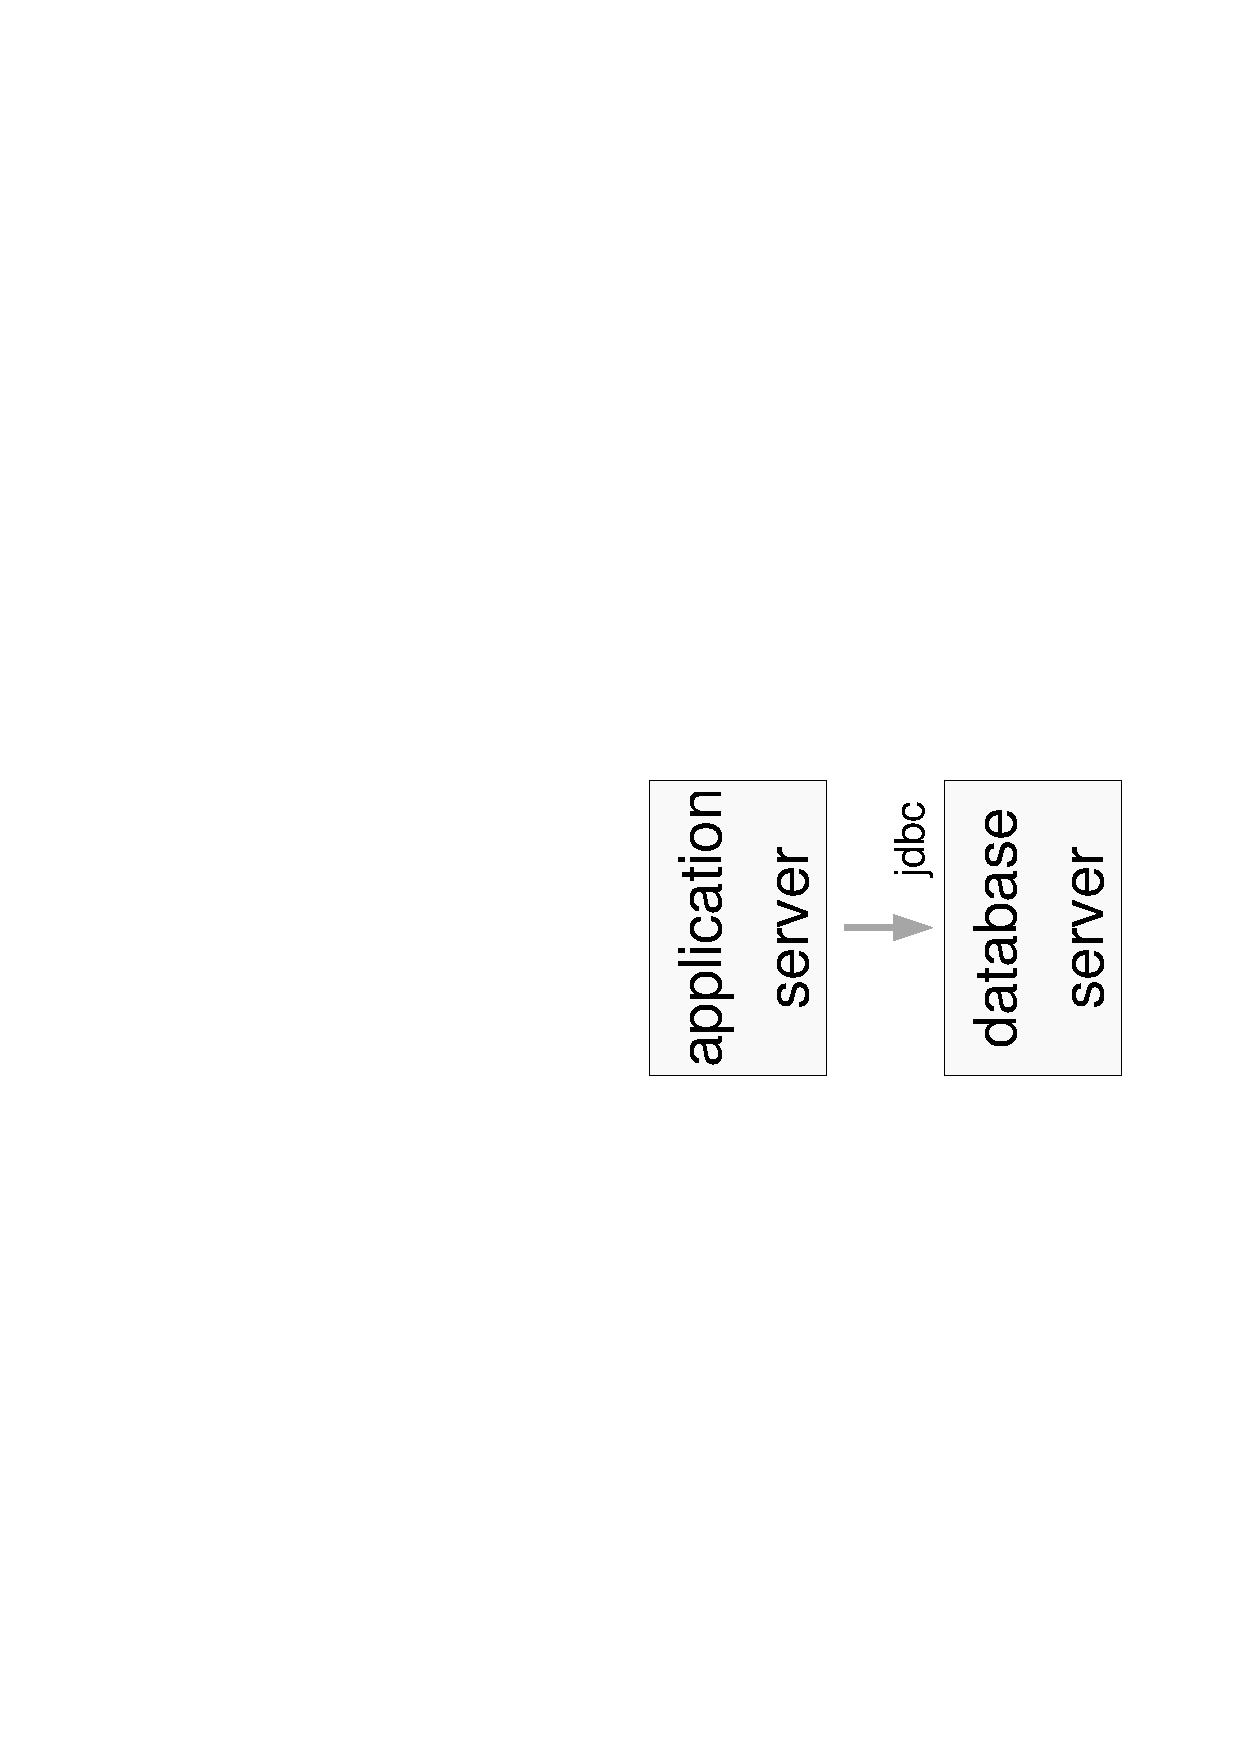
\includegraphics[scale=0.3,angle=-90]{graphic/database.pdf}
        \caption{Database Server (2 Tiers)}
        \label{database_figure}
    \end{center}
\end{figure}

\emph{Persistent Data} are those that live longer than the system working on them.
Very often, this is domain-specific- but also configuration information. These
are stored in a filesystem or database \cite{zimmermann}. \emph{Transient Data},
on the other hand, is temporary information that a system holds during its
lifetime, to function correctly. They get destroyed together with the system
which created them.

Managing persistent data implies a number of quite complex tasks, the details of
which will not be part of this document. To these aspects of database servers
belong:

\begin{itemize}
    \item[-] Querying
    \item[-] Transaction Handling
    \item[-] Locking
\end{itemize}

Different types of database systems exist. The major ones are:

\begin{itemize}
    \item[-] \emph{Hierarchical and Network DBMS}
    \item[-] \emph{Relational DBMS} (RDBMS)
    \item[-] \emph{Object-Relational DBMS} (ORDBMS)
    \item[-] \emph{Object-Oriented DBMS} (OODBMS)
\end{itemize}

Hierarchical DBMS were the first (electronic) databases ever used. They managed
their data in tree structures, starting each access from the root node. Network
DBMS went one step further: data could be associated at will \cite[p. 128]{zimmermann}.
Relational DBMS are based on tabular data structures which can have relations.
They were the first to accomplish a true separation between application and data.
Special languages were created to define and query such data sources: The
\emph{Data Definition Language} (DDL) and the \emph{Structured Query Language}
(SQL). Object-Relational DBMS were to fill the semantic gap between
\emph{Object-Oriented Model} (OOM) and \emph{Entity-Relationship Model} (ERM)
structures. Their extensions introduced a number of user-defined data types.
Object-Oriented DBMS conclusively close the semantic gap between object-oriented
applications and data. Their programming interface is often integrated into a
framework. The new SQL-based \emph{Object Query Language} (OQL)
\cite[p. 138]{zimmermann} was created for them.

The communication between systems can be eased with special techniques. After
Tanenbaum \cite{tanenbaum2002}, these were often called \emph{Middleware} since
they are placed between a higher-level layer consisting of users and applications,
and a layer underneath consisting of operating systems. In the case of database
systems, one such mechanism is the \emph{Java Database Connectivity} (JDBC)
\cite{hamilton, klute}; another one the \emph{Open Database Connectivity}
(ODBC) \cite[p. 170, 177]{zimmermann}. They provide a common interface for many
different relational databases.

Another technique are \emph{Enterprise Java Beans} (EJB) and comparable mechanisms.
They represent so-called \emph{Business Objects} (BO) and hence actually belong
to the previous section describing application servers. However, the containers
in which EJBs live also contain functionality for persistence- and transaction
handling which is why they are mentioned here. Further documentation can be found
in the corresponding literature \cite{gruhn} and sources \cite{blueprints, java}.

%
% $RCSfile: presentation_client.tex,v $
%
% Copyright (C) 2002-2008. Christian Heller.
%
% Permission is granted to copy, distribute and/or modify this document
% under the terms of the GNU Free Documentation License, Version 1.1 or
% any later version published by the Free Software Foundation; with no
% Invariant Sections, with no Front-Cover Texts and with no Back-Cover
% Texts. A copy of the license is included in the section entitled
% "GNU Free Documentation License".
%
% http://www.cybop.net
% - Cybernetics Oriented Programming -
%
% http://www.resmedicinae.org
% - Information in Medicine -
%
% Version: $Revision: 1.1 $ $Date: 2008-08-19 20:41:08 $ $Author: christian $
% Authors: Christian Heller <christian.heller@tuxtax.de>
%

\section{Presentation Client}
\label{presentation_client_heading}
\index{Presentation Client}
\index{Client}
\index{3 Tiers}
\index{Remote Method Invocation}
\index{RMI}
\index{Remote Procedure Call}
\index{RPC}
\index{Thin Client}
\index{Fat Client}
\index{Rich Client}

A system is called \emph{Client} when it uses services of a server. Most modern
applications incorporate abilities to communicate with server systems which may
run on the same computer as the client or on a remote machine that has to be
accessed over network.

\begin{figure}[ht]
    \begin{center}
        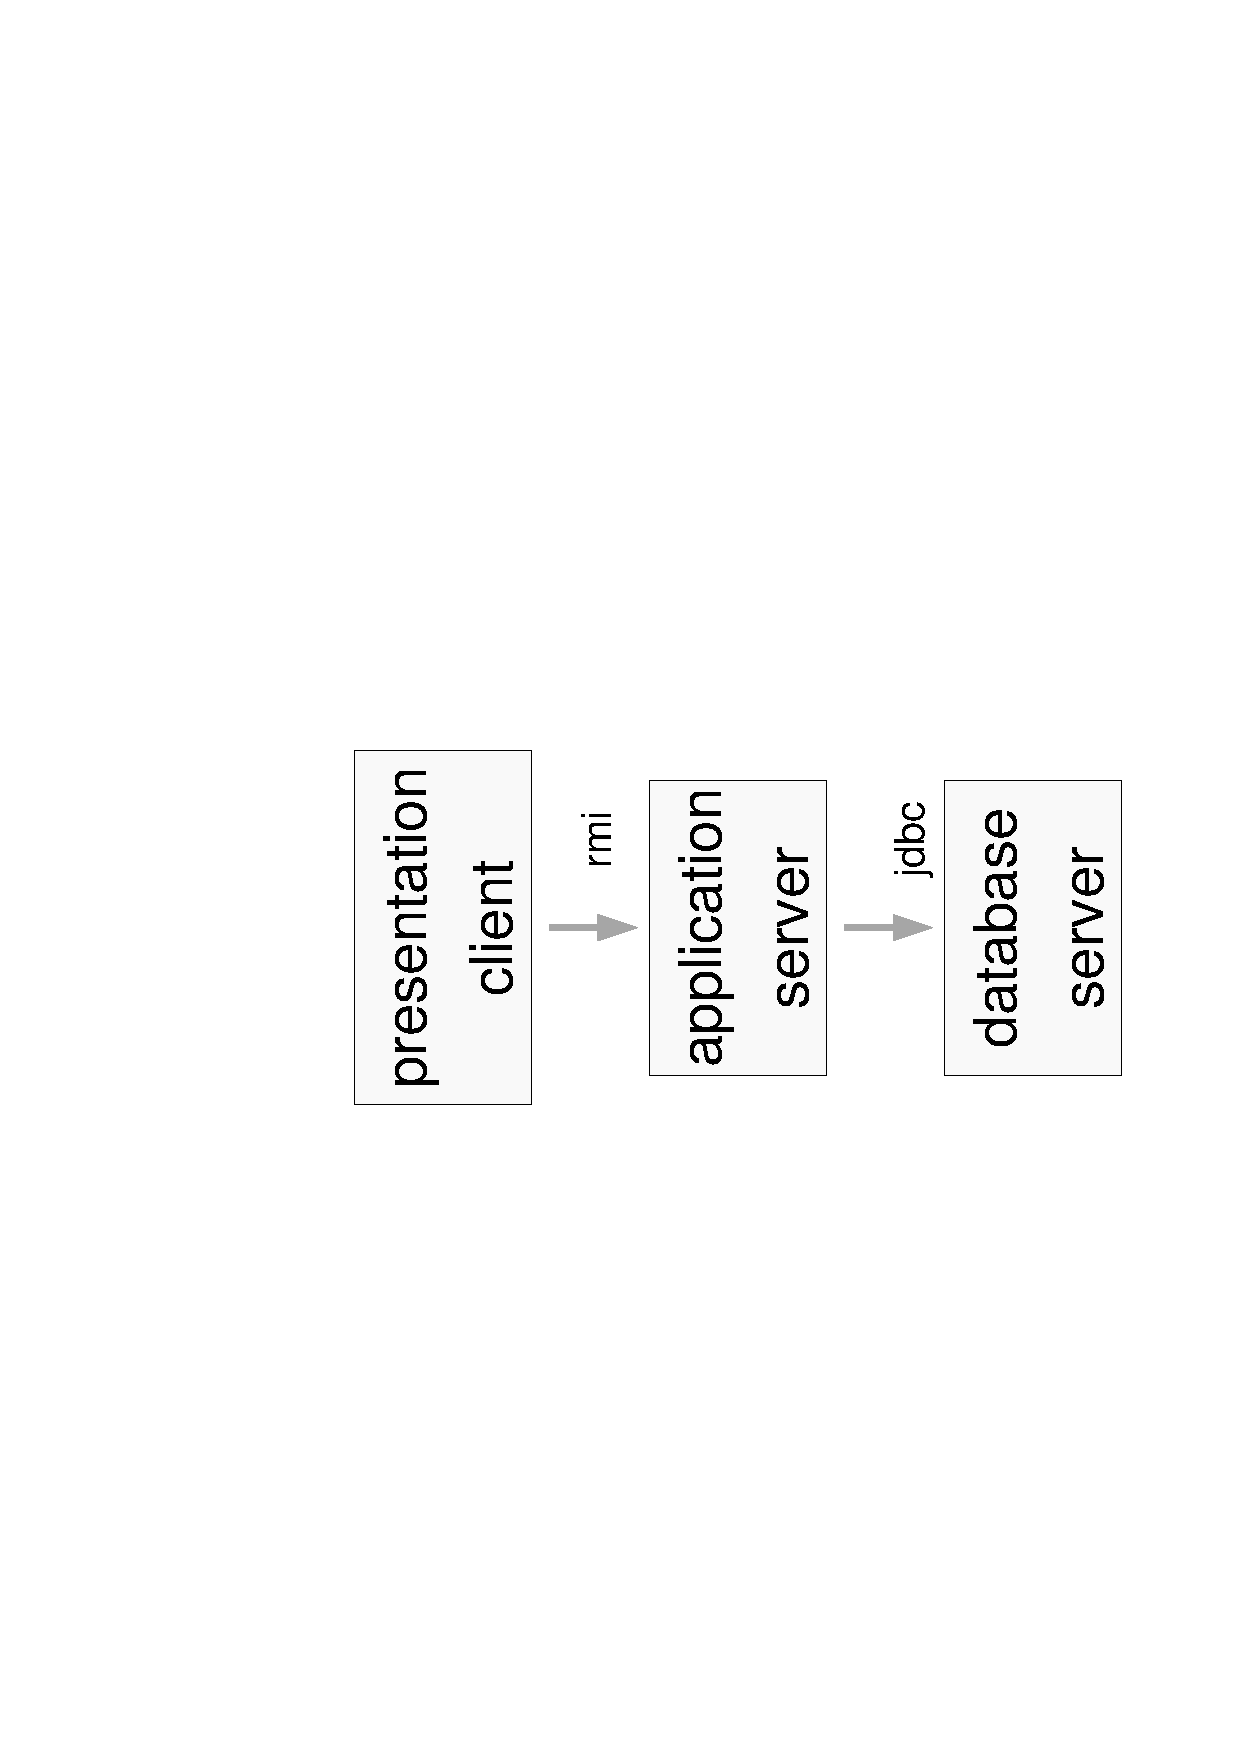
\includegraphics[scale=0.3,angle=-90]{graphic/client.pdf}
        \caption{Presentation Client (3 Tiers)}
        \label{client_figure}
    \end{center}
\end{figure}

But also clients can offer services as well as servers can use external services
and such become clients themselves. The application server in figure
\ref{database_figure} becomes a client when accessing the database system.
As can be seen -- \emph{Client} and \emph{Server} are quite arbitrary terms to
characterise systems.

Figure \ref{client_figure} illustrates the communication between a presentation
client and application server over network. Again, various mechanisms such as
\emph{Remote Method Invocation} (RMI), outside the Java world rather called
\emph{Remote Procedure Call} (RPC), exist to ease the way two remote systems
talk with one another.

Frequently, people distinguish between \emph{Thin Client} and \emph{Fat Client}
(the latter also called \emph{Rich Client}) \cite[p. 176]{zimmermann}. While a
thin client's task is nothing else than to display information coming from some
server, a fat client also takes over part of the business data processing which
is otherwise done by the server only.

%
% $RCSfile: web_client_and_server.tex,v $
%
% Copyright (C) 2002-2008. Christian Heller.
%
% Permission is granted to copy, distribute and/or modify this document
% under the terms of the GNU Free Documentation License, Version 1.1 or
% any later version published by the Free Software Foundation; with no
% Invariant Sections, with no Front-Cover Texts and with no Back-Cover
% Texts. A copy of the license is included in the section entitled
% "GNU Free Documentation License".
%
% http://www.cybop.net
% - Cybernetics Oriented Programming -
%
% http://www.resmedicinae.org
% - Information in Medicine -
%
% Version: $Revision: 1.1 $ $Date: 2008-08-19 20:41:09 $ $Author: christian $
% Authors: Christian Heller <christian.heller@tuxtax.de>
%

\section{Web Client and Server}
\label{web_client_and_server_heading}
\index{Web Client and Server}
\index{Internet}
\index{Web Server}
\index{Web Client}
\index{Web Browser}
\index{Applets}
\index{Servlets}
\index{Transfer Control Protocol}
\index{TCP}
\index{Internet Protocol}
\index{IP}
\index{Hypertext Transfer Protocol}
\index{HTTP}

With the emerge of the \emph{Internet}, several new kinds of services like
\emph{Email}, \emph{File Transfer}, \emph{Web} etc. became popular. The web
service allows information to be published in form of a \emph{Web Page}. Web
pages can be written in markup formats like \emph{Hypertext Markup Language}
(HTML) and \emph{Extensible Markup Language} (XML) or, using special tags, as
\emph{Java Server Pages-} (JSP) and \emph{PHP Hypertext Preprocessor-} (PHP)
instructions. Before being displayed, the latter two need to be translated by a
preprocessor inside the web server, into HTML.

\begin{figure}[ht]
    \begin{center}
        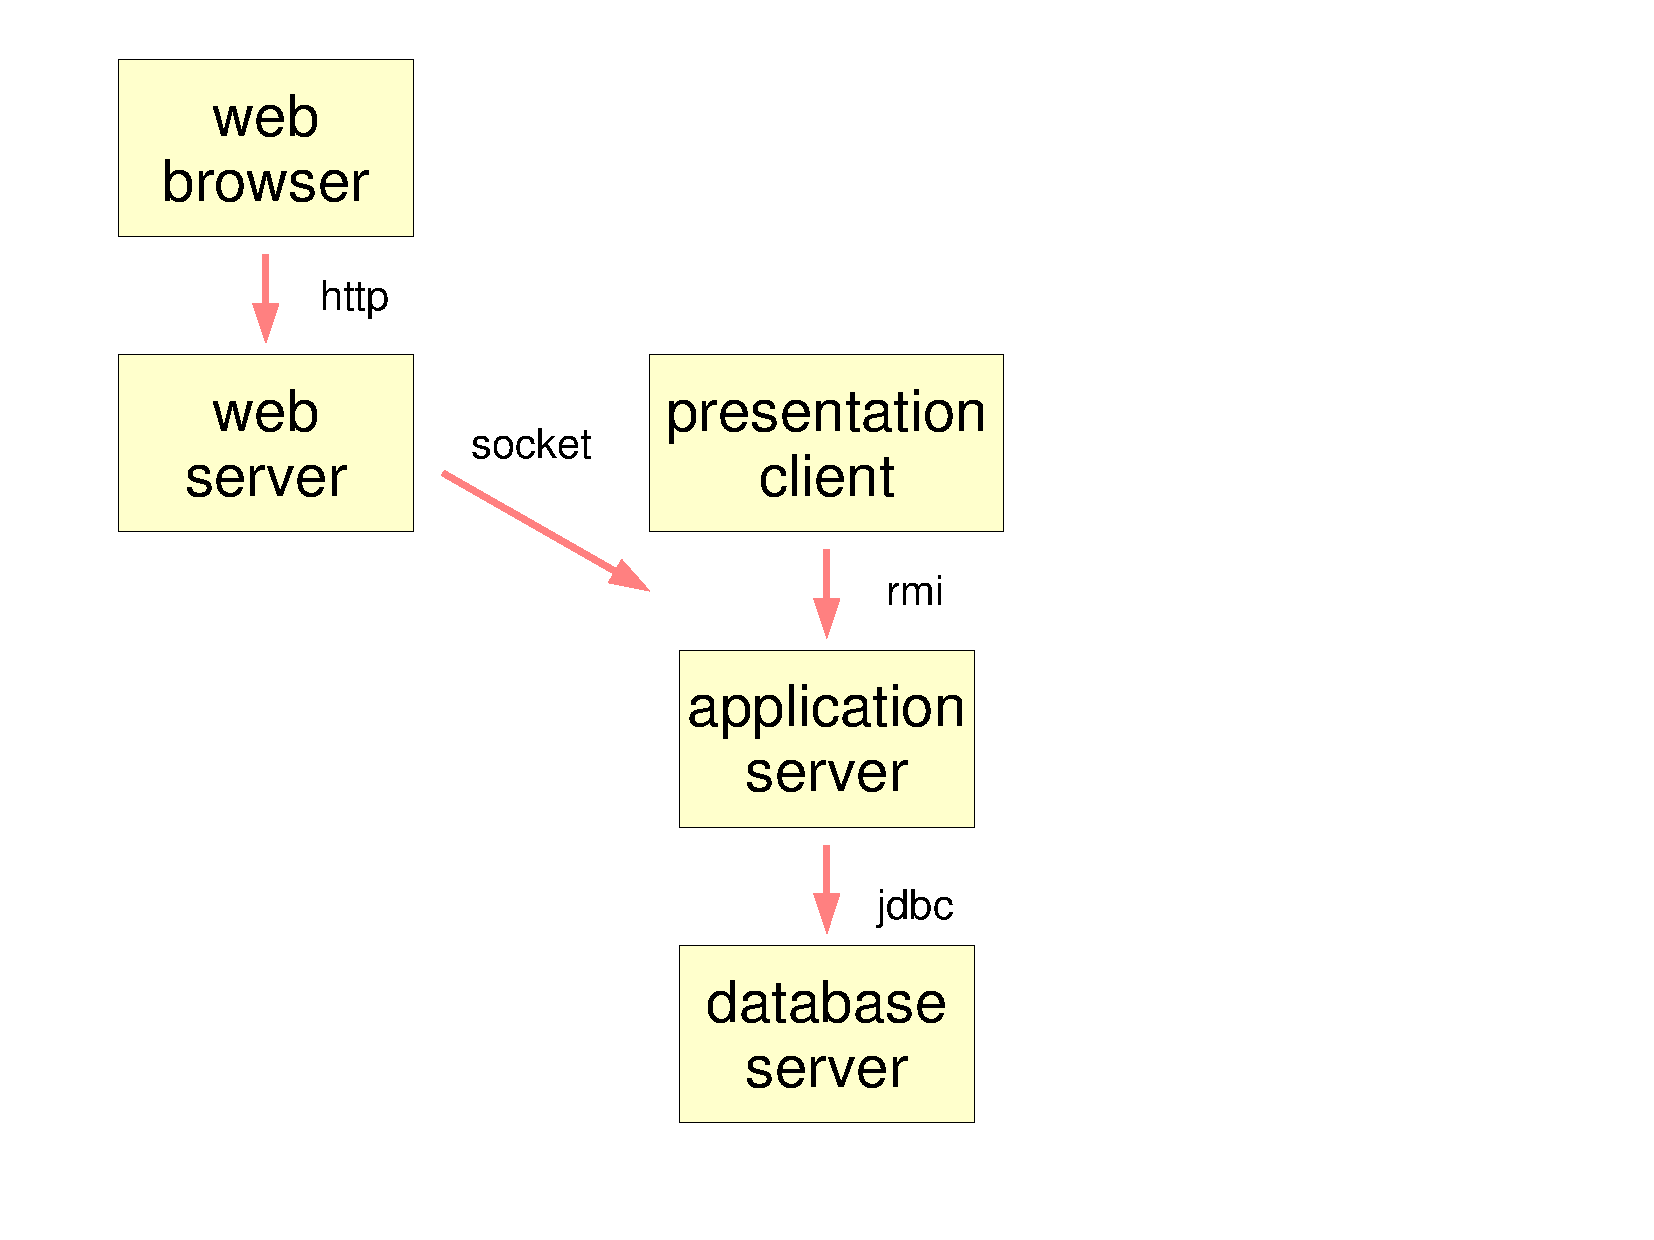
\includegraphics[scale=0.3,angle=-90]{graphic/web.pdf}
        \caption{Web Client and Server}
        \label{web_figure}
    \end{center}
\end{figure}

The principle as shown in figure \ref{web_figure} is easy: A \emph{Web Server}
stores web pages which can be accessed by clients called \emph{Web Browser}.
Browsers extract and translate (render) the (graphical) information given in
form of a web page and display them. But they are also able to handle actions
such as keyboard input or mouse click, and send these information back to the
web server.

Moreover, browsers can locally execute small programs called \emph{Applets}
which were downloaded from the web server. Their counterpart are \emph{Servlets}
which are executed in multiple threads on the web server, offering the actual
services.

Web communication is based on standards like the \emph{Transfer Control Protocol}/
\emph{Internet Protocol} (TCP/IP) and the \emph{Hypertext Transfer Protocol}
(HTTP) \cite{tanenbaum2000}. Section \ref{systems_interconnection_heading} will
systematise them together with other standards for system interconnection. The
socket mechanism may be used to connect a web server to an application server.

Many other aspects are important when talking about internet services. There is
the issue of security, there is performance, user-friendliness and many more
which will not be discussed further here, since it would exceed the frame of
this work.

%
% $RCSfile: local_process.tex,v $
%
% Copyright (C) 2002-2008. Christian Heller.
%
% Permission is granted to copy, distribute and/or modify this document
% under the terms of the GNU Free Documentation License, Version 1.1 or
% any later version published by the Free Software Foundation; with no
% Invariant Sections, with no Front-Cover Texts and with no Back-Cover
% Texts. A copy of the license is included in the section entitled
% "GNU Free Documentation License".
%
% http://www.cybop.net
% - Cybernetics Oriented Programming -
%
% http://www.resmedicinae.org
% - Information in Medicine -
%
% Version: $Revision: 1.1 $ $Date: 2008-08-19 20:41:07 $ $Author: christian $
% Authors: Christian Heller <christian.heller@tuxtax.de>
%

\section{Local Process}
\label{local_process_heading}
\index{Local Process}
\index{Nodes}
\index{Daemon}
\index{Small Servers}
\index{Inter-Process Communication}
\index{IPC}
\index{Dynamic Data Exchange}
\index{DDE}
\index{Object Linking and Embedding}
\index{OLE}
\index{ActiveX}
\index{Component Object Model}
\index{COM}
\index{Java Message Service}
\index{JMS}
\index{Desktop Communication Protocol}
\index{DCOP}
\index{Bonobo}
\index{Pipes}

Not all software systems run on physically separated computers, also called
\emph{Nodes}. And not all communication happens over network. As well, one
\emph{Local Process} can talk to a second on the same machine (figure
\ref{local_figure}). In fact, all applications have this ability, at least for
talking with the surrounding operating system.

\begin{figure}[ht]
    \begin{center}
        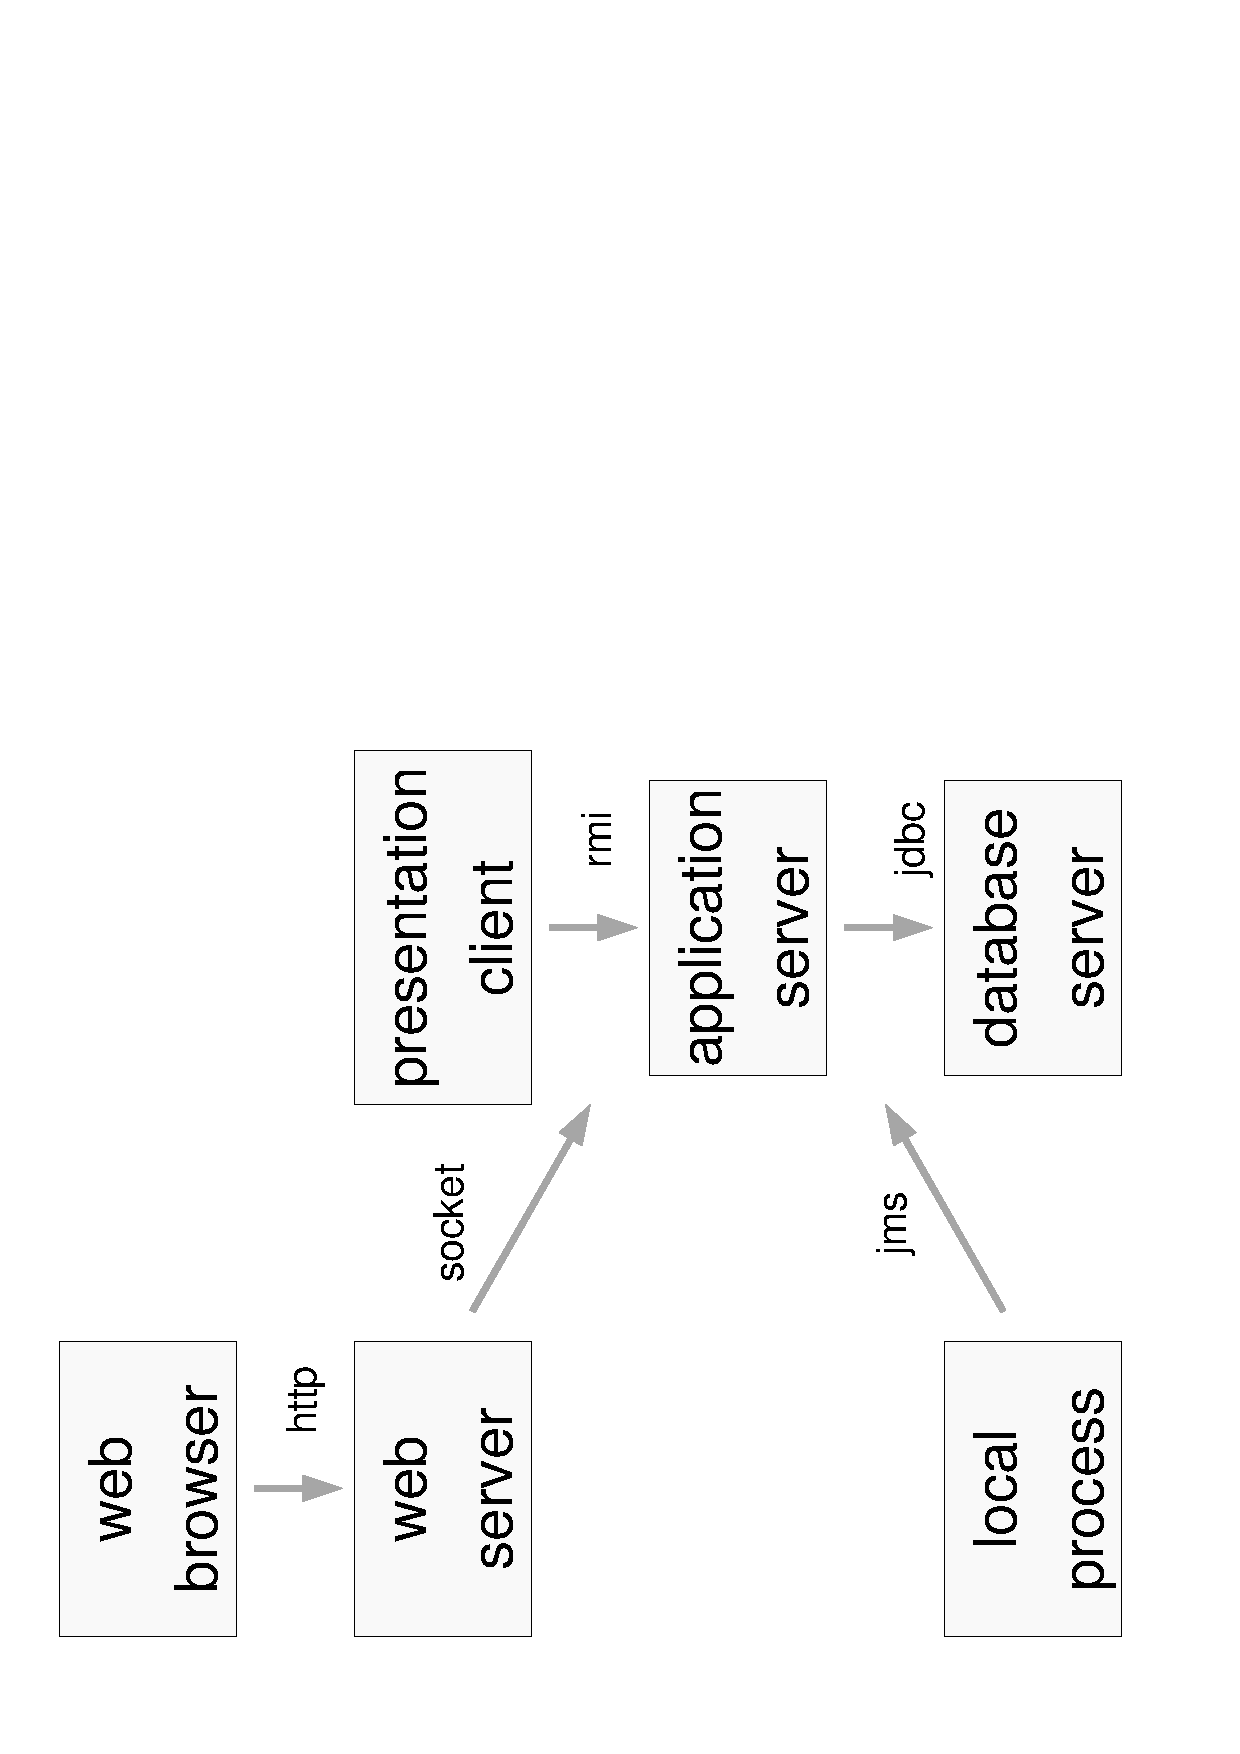
\includegraphics[scale=0.3,angle=-90]{graphic/local.pdf}
        \caption{Local Process}
        \label{local_figure}
    \end{center}
\end{figure}

Sometimes, local processes are needed by the operating system itself. Those are
running in the background then which is why they are often called \emph{Daemon}.
Because they offer special services, daemons are nothing else than small
servers. They fulfil tasks like managing all printing or email delivery of a
system, or similar things \cite[p. 74]{tanenbaum2001}.

Very often, it is useful to let local client applications talk with each other.
One part of a document (for instance a diagram) that was created by help of a
special application may want to get integrated into another document (for instance
a letter) which is edited by another application. A number of mechanisms were
created to solve this \emph{Inter-Process Communication} (IPC) task, for example:

\begin{itemize}
    \item[-] \emph{Dynamic Data Exchange} (DDE) \cite{ddefaq}
    \item[-] \emph{Object Linking and Embedding} (OLE/ OLE2) and \emph{ActiveX},
        both now based on the \emph{Component Object Model} (COM)
        \cite{zimmermann, gruhn}
    \item[-] \emph{Java Message Service} (JMS) \cite{java}
    \item[-] \emph{Desktop Communication Protocol} (DCOP) \cite{kde}
    \item[-] \emph{Bonobo} \cite{gnome}
    \item[-] \emph{Pipes} \cite{johnson, tanenbaum2001}
\end{itemize}

Although usually used for local communication (on the same node), some of these
also function over network. Again, this document will not discuss their inside
functionality. Plenty of books were written about that.

%
% $RCSfile: human_user.tex,v $
%
% Copyright (C) 2002-2008. Christian Heller.
%
% Permission is granted to copy, distribute and/or modify this document
% under the terms of the GNU Free Documentation License, Version 1.1 or
% any later version published by the Free Software Foundation; with no
% Invariant Sections, with no Front-Cover Texts and with no Back-Cover
% Texts. A copy of the license is included in the section entitled
% "GNU Free Documentation License".
%
% http://www.cybop.net
% - Cybernetics Oriented Programming -
%
% http://www.resmedicinae.org
% - Information in Medicine -
%
% Version: $Revision: 1.1 $ $Date: 2008-08-19 20:41:07 $ $Author: christian $
% Authors: Christian Heller <christian.heller@tuxtax.de>
%

\section{Human User}
\label{human_user_heading}
\index{Human User}
\index{Textual User Interface}
\index{TUI}
\index{Graphical User Interface}
\index{GUI}
\index{Human-Computer Interaction}
\index{HCI}

One system that needs special consideration is the \emph{Human User}. In the
first instance, it can be seen as normal system that is able to communicate
with other humans but also with artificial software systems running on machines
such as computers (figure \ref{user_figure}).

\begin{figure}[ht]
    \begin{center}
        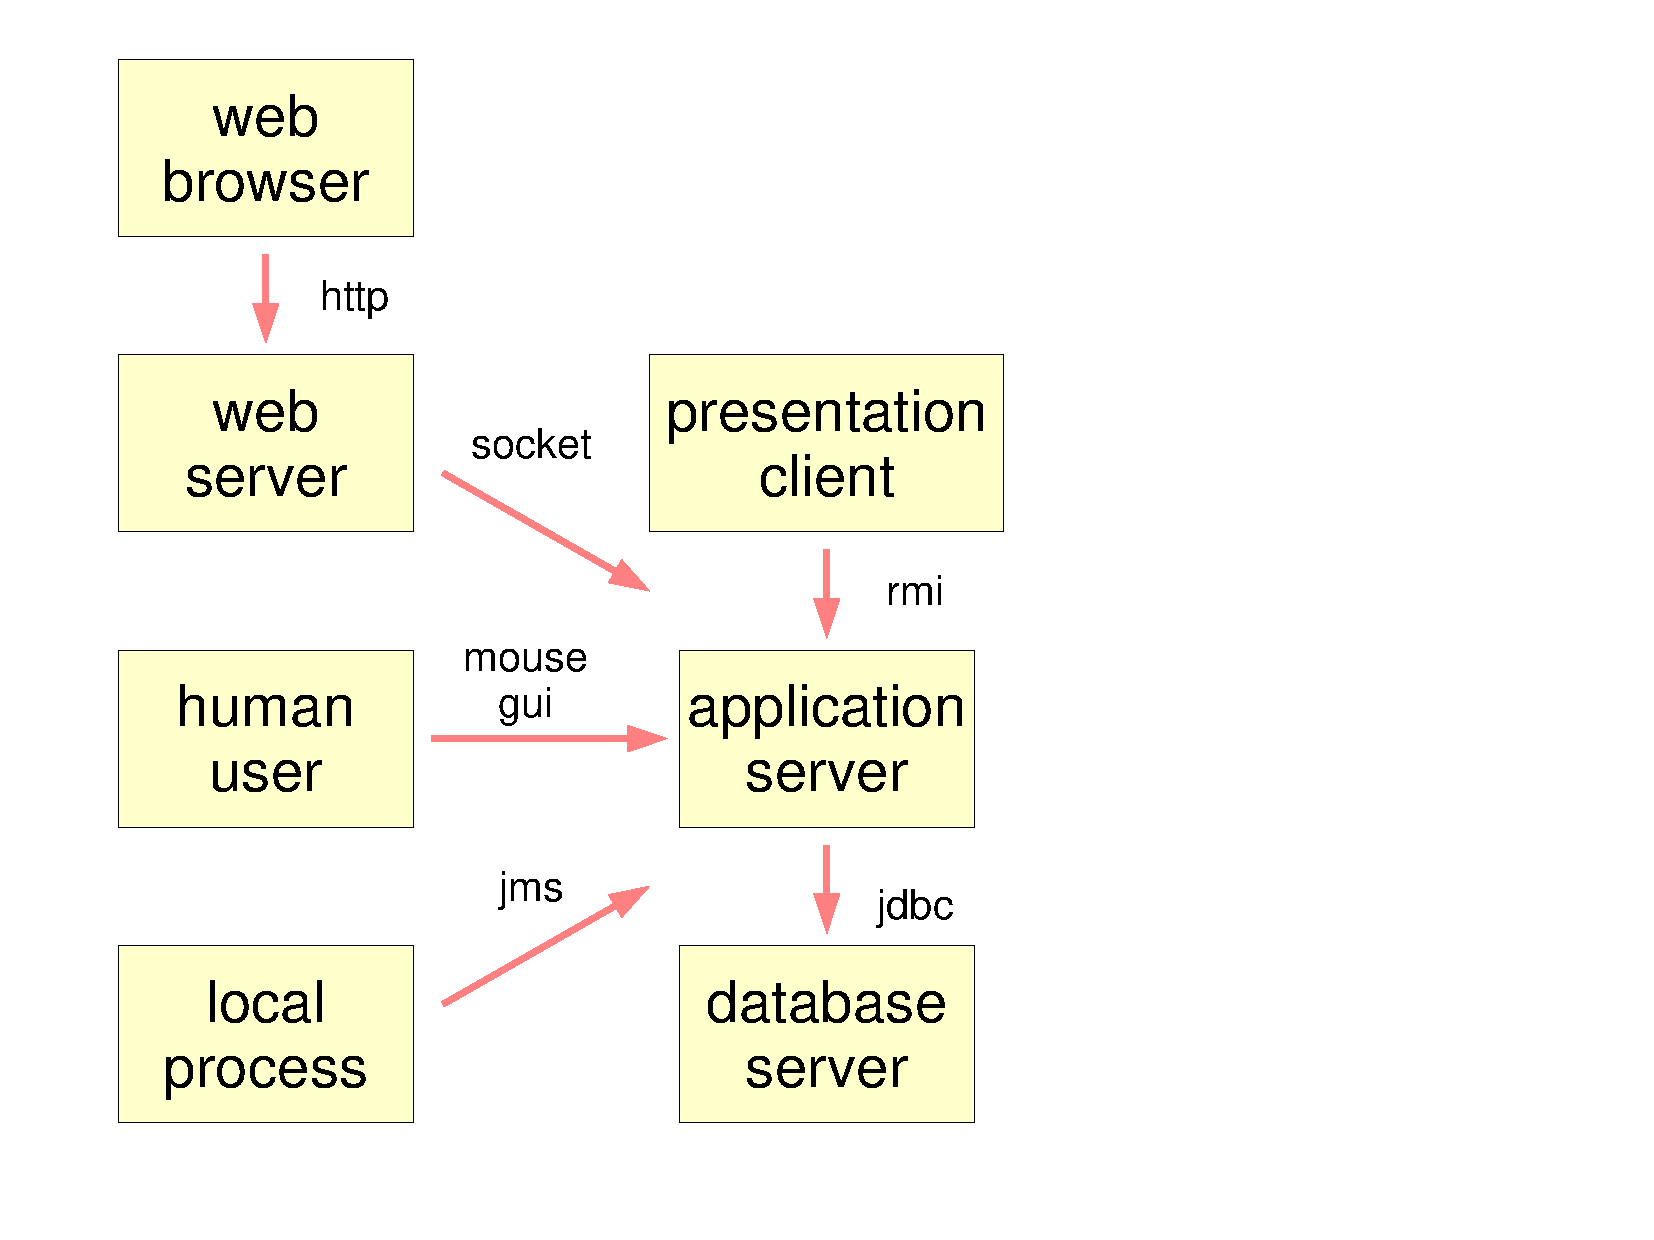
\includegraphics[scale=0.3,angle=-90]{graphic/user.pdf}
        \caption{Human User}
        \label{user_figure}
    \end{center}
\end{figure}

At the second view, one realises that due to the difference in construction,
human systems rely on other kinds of communication signals. While network cards
are usually enough for two computers to exchange data, additional input/ output
devices are needed to let human beings and computers talk to each other. To these
devices count: \emph{Keyboard}, \emph{Mouse}, \emph{Screen}, \emph{Printer} and
many more. They are made to suit the five human senses, that is to generate and
understand optical, acoustical, mechanical and similar signals.

The optical information displayed on a screen is often systematised into
character-based \emph{Textual User Interface} (TUI) and window-based
\emph{Graphical User Interface} (GUI).

The scientific subject dealing with those issues in more detail is called
\emph{Human-Computer Interaction} (HCI). One working definition given in
\cite{sigchi} states:

\begin{quote}
    Human-computer interaction is a discipline concerned with the design,
    evaluation and implementation of interactive computing systems for human
    use and with the study of major phenomena surrounding them.
\end{quote}

%
% $RCSfile: peer_node.tex,v $
%
% Copyright (C) 2002-2008. Christian Heller.
%
% Permission is granted to copy, distribute and/or modify this document
% under the terms of the GNU Free Documentation License, Version 1.1 or
% any later version published by the Free Software Foundation; with no
% Invariant Sections, with no Front-Cover Texts and with no Back-Cover
% Texts. A copy of the license is included in the section entitled
% "GNU Free Documentation License".
%
% http://www.cybop.net
% - Cybernetics Oriented Programming -
%
% http://www.resmedicinae.org
% - Information in Medicine -
%
% Version: $Revision: 1.1 $ $Date: 2008-08-19 20:41:08 $ $Author: christian $
% Authors: Christian Heller <christian.heller@tuxtax.de>
%

\section{Peer Node}
\label{peer_node_heading}
\index{Peer Node}
\index{Distributed System}
\index{Distributed Computing Environment}
\index{DCE}
\index{c/s}
\index{Peer-to-Peer}
\index{P2P}
\index{Client}
\index{Server}
\index{Freenet}
\index{Gnutella}
\index{BitTorrent}
\index{eDonkey}
\index{FastTrack}
\index{Napster}

Tanenbaum and Steen \cite{tanenbaum2002} define a \emph{Distributed System} as
\textit{a collection of independent computers that appear to its users as a
single coherent system}. With \emph{System} referring to a process rather than
only hardware, as defined in section \ref{process_heading}, it seems appropriate
to rephrase and use this for the definition of a general
\emph{Distributed Computing Environment} (DCE):

\begin{quote}
    A distributed computing environment consists of at least two systems that
    work together over a network but run on independent computer hardware (nodes).
\end{quote}

\begin{figure}[ht]
    \begin{center}
        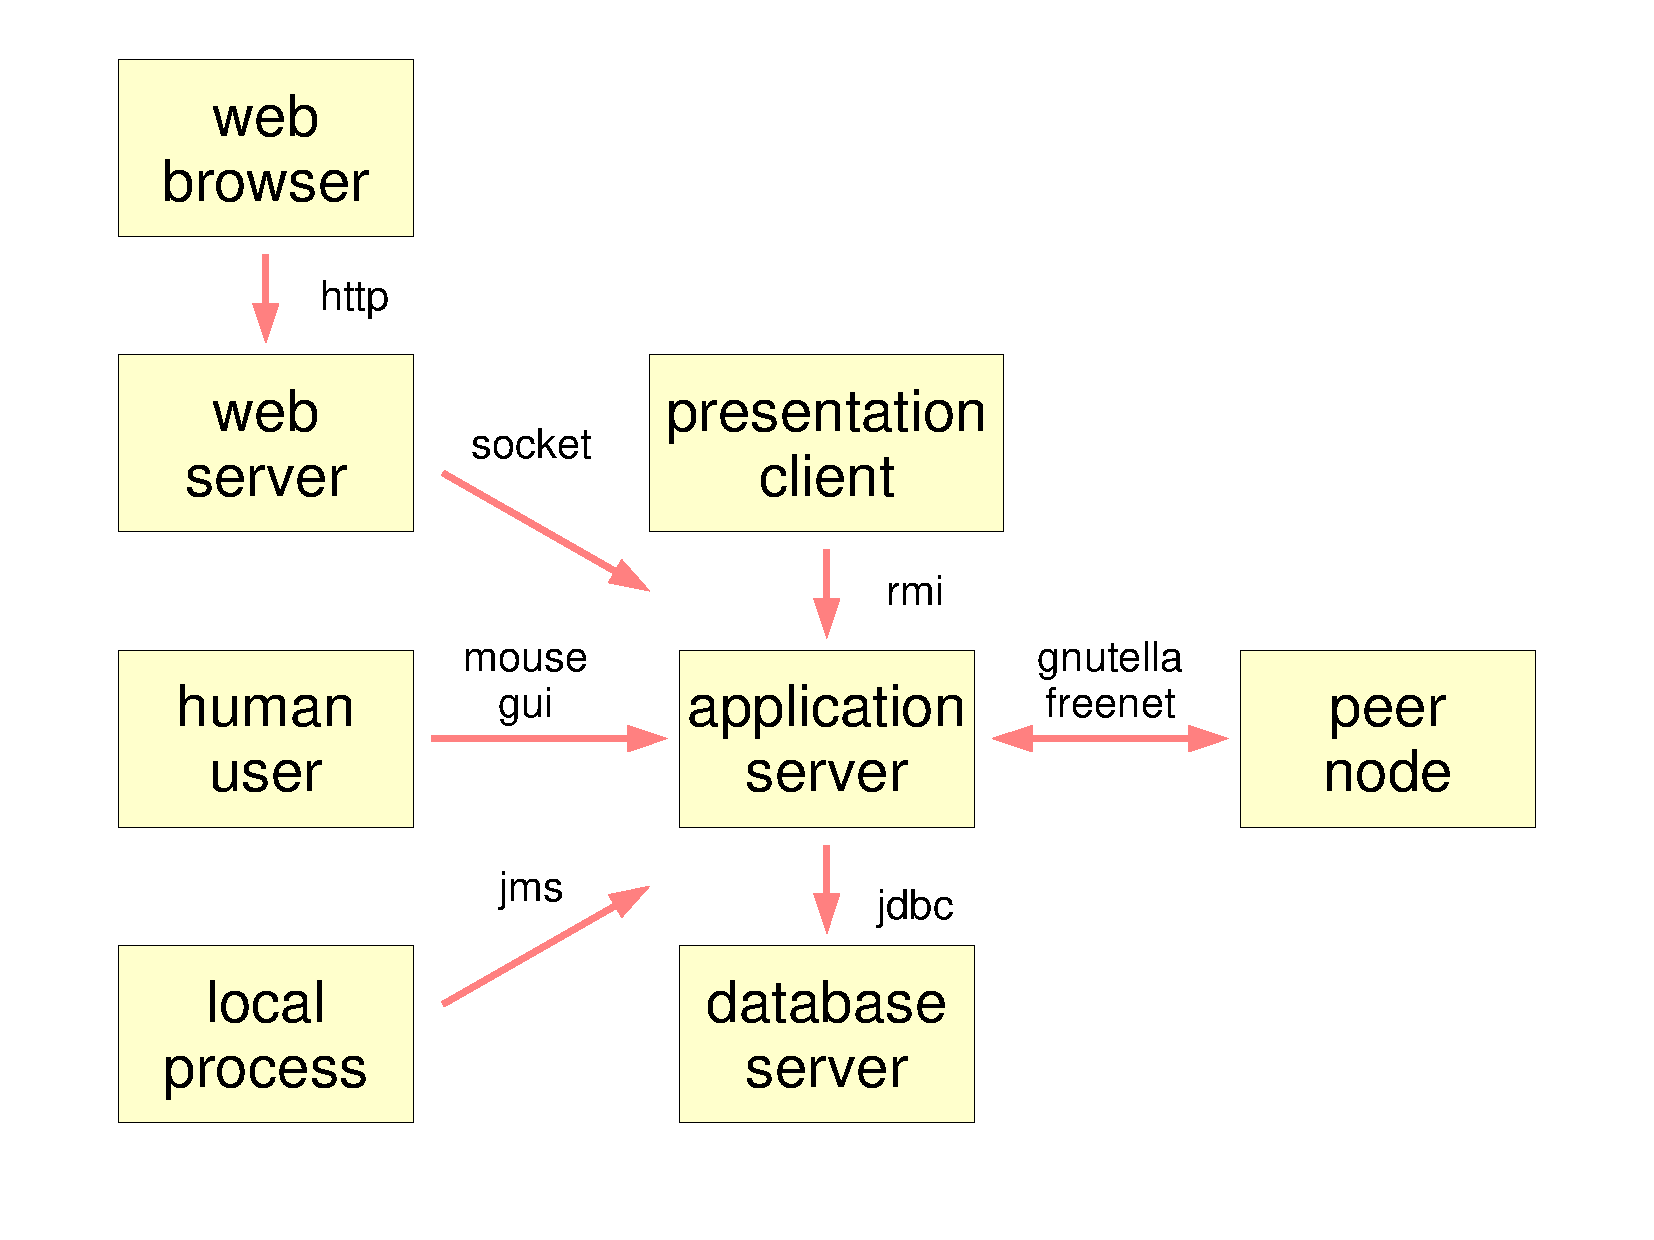
\includegraphics[scale=0.3,angle=-90]{graphic/peer.pdf}
        \caption{Peer-to-Peer Node Communication}
        \label{peer_figure}
    \end{center}
\end{figure}

Besides the previously mentioned client/ server (c/s) environments, so-called
\emph{Peer-to-Peer} (P2P) computer networks latterly became popular. In them,
nodes do not have just one role, but act as client and server at the same time
(figure \ref{peer_figure}), thus sharing their computing power and bandwidth.
Common P2P protocols are: \emph{Freenet}, \emph{Gnutella2}, \emph{BitTorrent},
\emph{eDonkey}, \emph{FastTrack} or \emph{Napster} \cite{wikipedia}. Many more
exist.

Just like nodes in a P2P network, human beings are capable of communicating
both ways, taking the role of a client or server. The organs that are needed to
do so are put into comparison with the corresponding devices of a computer
system, in chapter \ref{state_and_logic_heading}.

%
% $RCSfile: remote_server.tex,v $
%
% Copyright (C) 2002-2008. Christian Heller.
%
% Permission is granted to copy, distribute and/or modify this document
% under the terms of the GNU Free Documentation License, Version 1.1 or
% any later version published by the Free Software Foundation; with no
% Invariant Sections, with no Front-Cover Texts and with no Back-Cover
% Texts. A copy of the license is included in the section entitled
% "GNU Free Documentation License".
%
% http://www.cybop.net
% - Cybernetics Oriented Programming -
%
% http://www.resmedicinae.org
% - Information in Medicine -
%
% Version: $Revision: 1.1 $ $Date: 2008-08-19 20:41:08 $ $Author: christian $
% Authors: Christian Heller <christian.heller@tuxtax.de>
%

\section{Remote Server}
\label{remote_server_heading}
\index{Remote Server}
\index{Streams}
\index{Common Object Request Broker Architecture}
\index{CORBA}
\index{Simple Object Access Protocol}
\index{SOAP}
\index{Network Dynamic Data Exchange}
\index{NetDDE}
\index{Distributed Component Object Model}
\index{DCOM}
\index{COM+}
\index{KParts}
\index{Universal Network Objects}
\index{UNO}

Figure \ref{remote_figure} introduces a \emph{Remote Server} to the illustrated
example environment. It may access a database system -- similarly to the already
existing application server. In this example, however, it just works on simple
local files, using \emph{Streams}.

\begin{figure}[ht]
    \begin{center}
        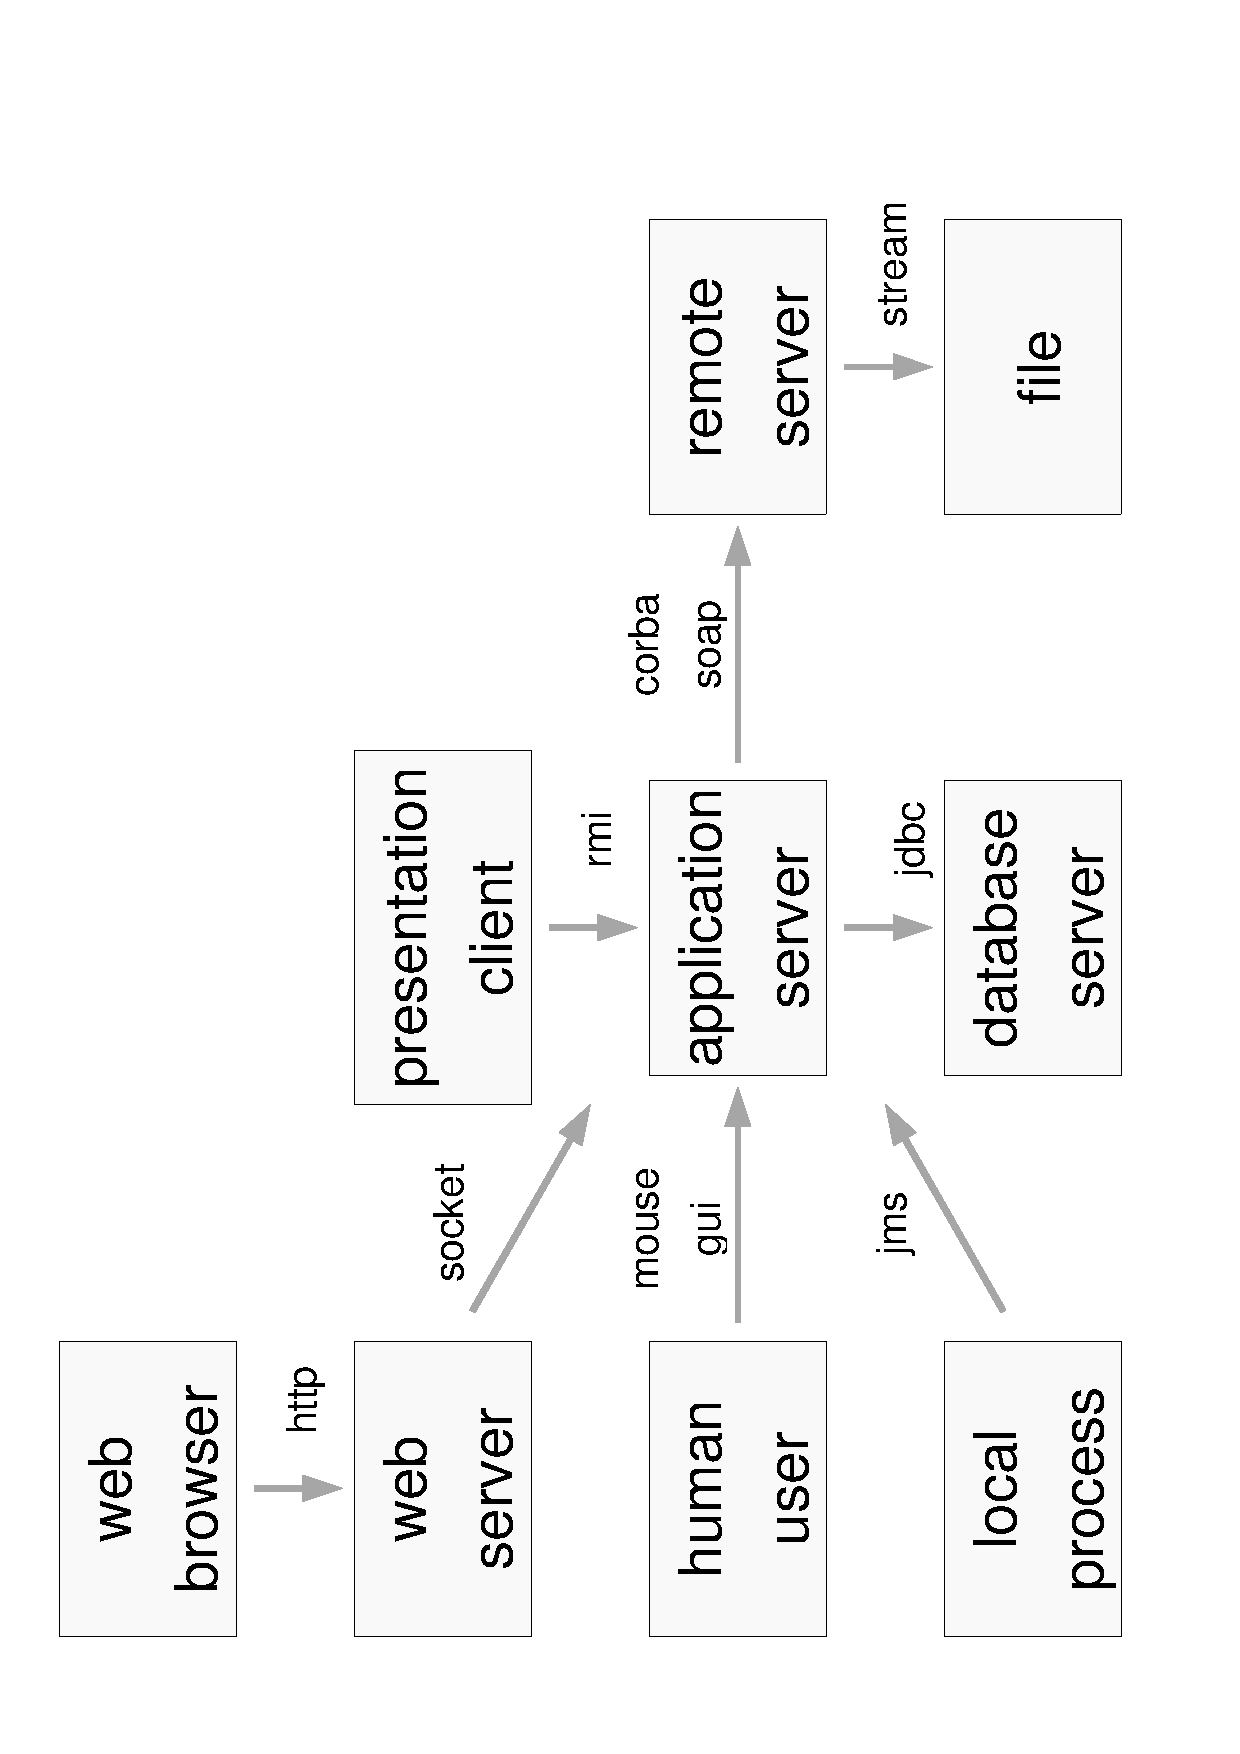
\includegraphics[scale=0.3,angle=-90]{graphic/remote.pdf}
        \caption{Remote Server}
        \label{remote_figure}
    \end{center}
\end{figure}

Like the previously introduced kinds of systems, remote systems need to rely on
a number of standards and mechanisms, in order to be able to communicate over
network. A comparison of some of these is given in \cite{olson, brownech, hrastnik}.
In the following is a list of common techniques that were not yet mentioned
before:

\begin{itemize}
    \item[-] \emph{Common Object Request Broker Architecture} (CORBA)
        \cite{corba, vinoski, gruhn}
    \item[-] \emph{Simple Object Access Protocol} (SOAP) \cite{soap}
    \item[-] \emph{Network Dynamic Data Exchange} (NetDDE) \cite{ddefaq}
    \item[-] \emph{Distributed Component Object Model} (DCOM/ COM+) \cite{gruhn}
    \item[-] \emph{KParts} \cite{kde}
    \item[-] \emph{Universal Network Objects} (UNO) \cite{openoffice}
\end{itemize}

%
% $RCSfile: legacy_host.tex,v $
%
% Copyright (C) 2002-2008. Christian Heller.
%
% Permission is granted to copy, distribute and/or modify this document
% under the terms of the GNU Free Documentation License, Version 1.1 or
% any later version published by the Free Software Foundation; with no
% Invariant Sections, with no Front-Cover Texts and with no Back-Cover
% Texts. A copy of the license is included in the section entitled
% "GNU Free Documentation License".
%
% http://www.cybop.net
% - Cybernetics Oriented Programming -
%
% http://www.resmedicinae.org
% - Information in Medicine -
%
% Version: $Revision: 1.1 $ $Date: 2008-08-19 20:41:07 $ $Author: christian $
% Authors: Christian Heller <christian.heller@tuxtax.de>
%

\section{Legacy Host}
\label{legacy_host_heading}
\index{Legacy Host}
\index{Legacy Systems}
\index{Host}
\index{Mainframe}
\index{Common Business Oriented Language}
\index{COBOL}
\index{Programming Language One}
\index{PL/I}
\index{Virtual Storage Access Method}
\index{VSAM}
\index{Third Party Maintenance}
\index{TPM}
\index{Customer Information Control System}
\index{CICS}

Finally, there is often a need to integrate \emph{Legacy Systems}, which are a
special variant of remote software systems running on computers with an older
architecture. Those computers are also named \emph{Host}, as in the example of
figure \ref{legacy_figure}, or \emph{Mainframe}. The applications running on
them are programmed in languages like the \emph{Common Business Oriented Language}
(COBOL) or \emph{Programming Language One} (PL/I) \cite{pli}, the latter
developed as an \emph{International Business Machines} (IBM) \cite{ibm} product
in the mid 1960's.

\begin{figure}[ht]
    \begin{center}
        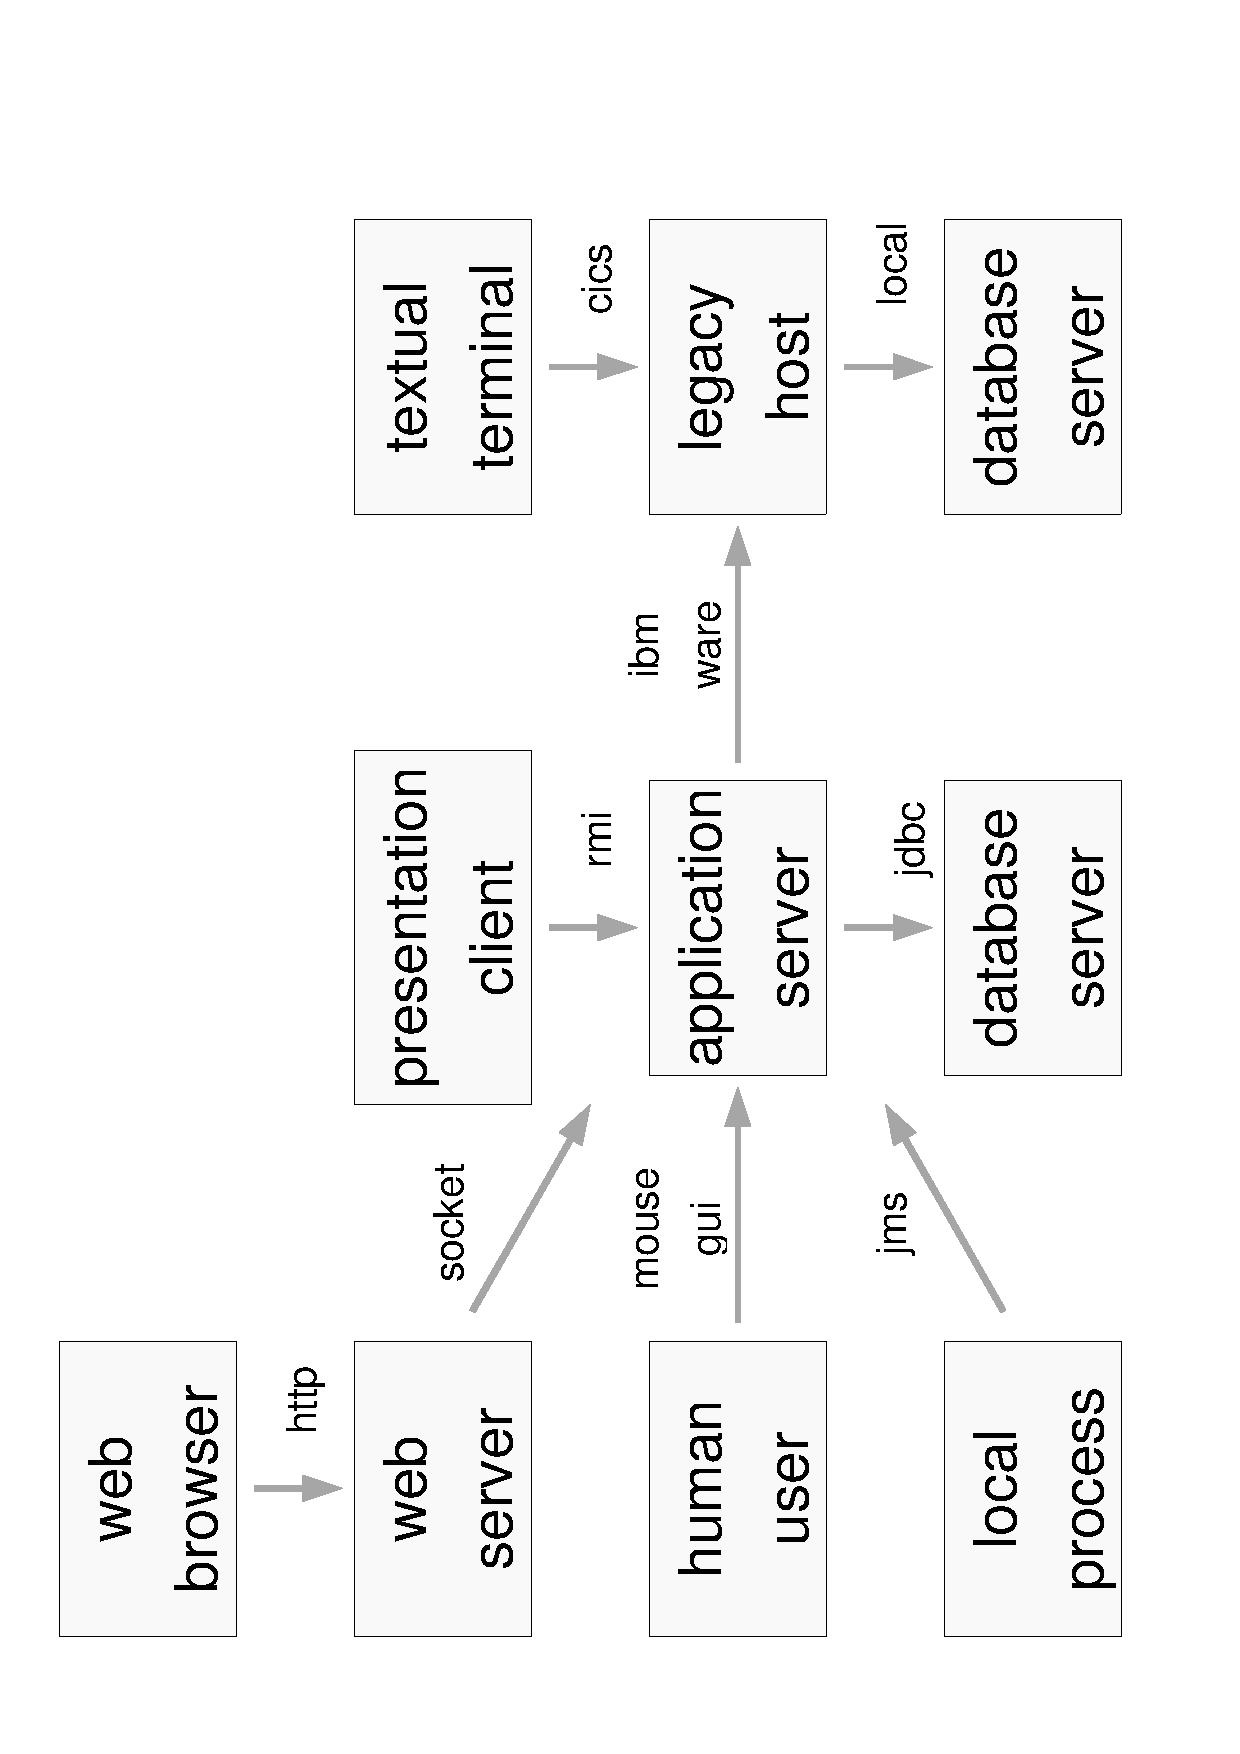
\includegraphics[scale=0.3,angle=-90]{graphic/legacy.pdf}
        \caption{Legacy Host}
        \label{legacy_figure}
    \end{center}
\end{figure}

Host computers manage nearly everything an ancient information technology
environment needs. They are responsible for persistence and processing of data.
Often, they contain hierarchical databases \cite{oolegacysystems} using flat
files like the \emph{Virtual Storage Access Method} (VSAM) format. True clients
do not exist here. Character-based terminals are the way to communicate with
the host which controls all interaction (including keyboard and screen), within
a \emph{Third Party Maintenance} (TPM) \emph{Customer Information Control System}
(CICS) runtime environment.

%
% $RCSfile: systems_interconnection.tex,v $
%
% Copyright (C) 2002-2008. Christian Heller.
%
% Permission is granted to copy, distribute and/or modify this document
% under the terms of the GNU Free Documentation License, Version 1.1 or
% any later version published by the Free Software Foundation; with no
% Invariant Sections, with no Front-Cover Texts and with no Back-Cover
% Texts. A copy of the license is included in the section entitled
% "GNU Free Documentation License".
%
% http://www.cybop.net
% - Cybernetics Oriented Programming -
%
% http://www.resmedicinae.org
% - Information in Medicine -
%
% Version: $Revision: 1.1 $ $Date: 2008-08-19 20:41:09 $ $Author: christian $
% Authors: Christian Heller <christian.heller@tuxtax.de>
%

\section{Systems Interconnection}
\label{systems_interconnection_heading}
\index{Systems Interconnection}
\index{Open Systems Interconnection}
\index{OSI}
\index{International Organization for Standardization}
\index{ISO OSI Reference Model}
\index{Simple Mail Transfer Protocol}
\index{SMTP}
\index{Telephone Network}
\index{Telnet}
\index{File Transfer Protocol}
\index{FTP}
\index{Hypertext Transfer Protocol}
\index{HTTP}
\index{Domain Name Service}
\index{DNS}
\index{X.226}
\index{Remote Procedure Call}
\index{RPC}
\index{Network Basic Input/ Output System}
\index{NetBIOS}
\index{Transfer Control Protocol}
\index{TCP}
\index{User Datagram Protocol}
\index{UDP}
\index{Transport Protocol Class 4}
\index{TP4}
\index{Sequence Package Exchange}
\index{SPX}
\index{Internet Protocol}
\index{IP}
\index{Internet Packet Exchange}
\index{IPX}
\index{Point-to-Point Protocol}
\index{PPP}
\index{Serial Line Internet Protocol}
\index{SLIP}
\index{Frame Relay}
\index{FR}
\index{X.25}
\index{Ethernet}
\index{Token Ring}
\index{Fiber Distributed Data Interface}
\index{FDDI}
\index{Ontology}
\index{Health Level Seven}
\index{HL7}
\index{TCP/IP}
\index{Universal Interactive Executive}
\index{UNIX}
\index{Operating System}
\index{OS}

Communication is essential to an IT environment as described before. To enable
and ease communication across different systems, special solutions have been
developed and accepted as \emph{de facto} or \emph{de jure} standards. One such
specification is the well-known \emph{Open Systems Interconnection} (OSI)
reference model, defined by the \emph{International Organization for Standardization}
(ISO). Numerous books \cite{tanenbaum2000} and documents on the web
\cite{payer} describe this model and its protocols.

\begin{figure}[ht]
    \begin{center}
        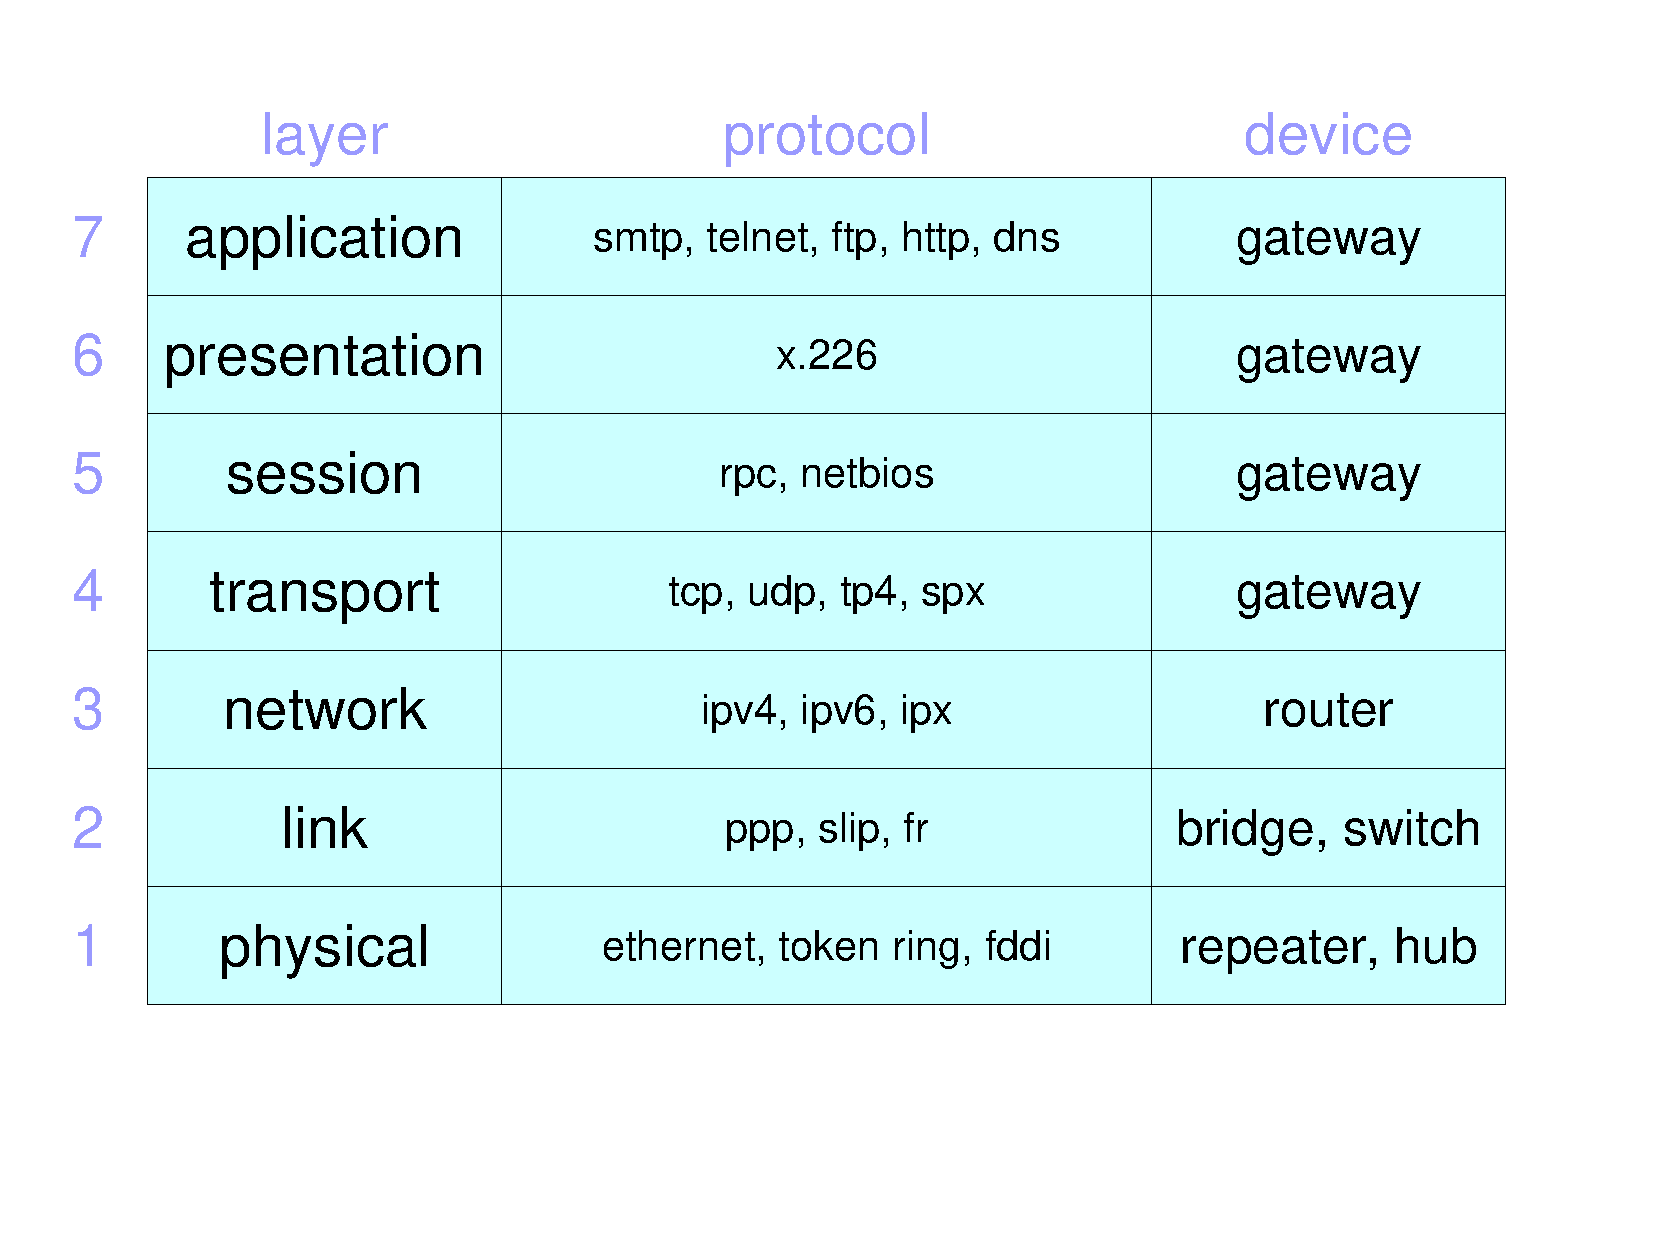
\includegraphics[scale=0.3,angle=-90]{graphic/osi.pdf}
        \caption{ISO OSI Reference Model}
        \label{osi_figure}
    \end{center}
\end{figure}

Figure \ref{osi_figure} organises the seven layers of the model in table form,
with one row representing one layer. The first column contains a layer's name,
the second examples of typical network protocols and the third devices in which
the protocols are used. \emph{Simple Mail Transfer Protocol} (SMTP),
\emph{Telephone Network} (Telnet), \emph{File Transfer Protocol} (FTP),
\emph{Hypertext Transfer Protocol} (HTTP) and \emph{Domain Name Service} (DNS)
are standard protocols used directly in software applications and -tools.
\emph{X.226} is a recommendation defining the OSI presentation protocol. The
\emph{Remote Procedure Call} (RPC) and \emph{Network Basic Input/ Output System}
(NetBIOS) may be sorted into the session layer. \emph{Transfer Control Protocol}
(TCP), \emph{User Datagram Protocol} (UDP), \emph{Transport Protocol Class 4}
(TP4) and \emph{Sequence Package Exchange} (SPX) do belong to the transport
layer. The \emph{Internet Protocol} (IP) is used in two versions: 4 and 6. Both
of them are situated on the network level of the OSI model, just like the
\emph{Internet Packet Exchange} (IPX) protocol. The link level contains the
\emph{Point-to-Point Protocol} (PPP), \emph{Serial Line Internet Protocol}
(SLIP) and \emph{Frame Relay} (FR), the latter being a replacement for veterans
like \emph{X.25}. To the physical level transmitting raw Bits finally, belong
\emph{Ethernet}, \emph{Token Ring} and \emph{Fiber Distributed Data Interface}
(FDDI).

Many of the mentioned protocols may be assigned to more than just one layer.
But it is \emph{not} the intention of this work to deal with such details. The
overall ISO OSI model, however, is mentioned because it is a good example of a
structure whose layers represent increasing levels of abstraction, what will
later in this work be called an \emph{Ontology} (chapters
\ref{logical_architecture_heading} and \ref{knowledge_schema_heading}). Also,
the \emph{Health Level Seven} (HL7) medical standard, which gets introduced in
chapter \ref{res_medicinae_heading}, received its name from referring to OSI's
seventh level -- the application level \cite{rogers}.

While the ISO OSI model defines seven abstract communication layers, the
popular \emph{TCP/IP} model uses solely four. Web communication as described in
section \ref{web_client_and_server_heading} is based on it. Today, TCP/IP has
become the standard in network management systems. A majority of them run the
\emph{Universal Interactive Executive} (UNIX) \emph{Operating System} (OS), of
which TCP/IP is an integral part. Margarete Payer \cite{payer} writes:
\textit{Although the OSI Model is affected with various deficiencies, it is
well suitable for didactic purposes.} Further, she mentions that since some
time, Andrew S. Tanenbaum uses a hybrid model for structuring his standard book
on computer networks \cite{tanenbaum2000}, which sticked to neither OSI nor
TCP/IP.

%
% $RCSfile: scalability.tex,v $
%
% Copyright (C) 2002-2008. Christian Heller.
%
% Permission is granted to copy, distribute and/or modify this document
% under the terms of the GNU Free Documentation License, Version 1.1 or
% any later version published by the Free Software Foundation; with no
% Invariant Sections, with no Front-Cover Texts and with no Back-Cover
% Texts. A copy of the license is included in the section entitled
% "GNU Free Documentation License".
%
% http://www.cybop.net
% - Cybernetics Oriented Programming -
%
% http://www.resmedicinae.org
% - Information in Medicine -
%
% Version: $Revision: 1.1 $ $Date: 2008-08-19 20:41:08 $ $Author: christian $
% Authors: Christian Heller <christian.heller@tuxtax.de>
%

\section{Scalability}
\label{scalability_heading}
\index{Scalability}
\index{Vertical Scaling}
\index{Horizontal Scaling}
\index{Symmetric Multiprocessing}
\index{SMP}
\index{Central Processing Units}
\index{CPU}
\index{Operating System}
\index{OS}
\index{Input/ Output}
\index{i/o}
\index{Reliability, Availability, Serviceability}
\index{RAS}
\index{Clustering}
\index{Vertical System}
\index{Horizontal System}
\index{Large Database}
\index{Web Server}
\index{Transactional Database}
\index{Firewall}
\index{Data Warehouse}
\index{Proxy Server}
\index{Data Mining}
\index{Directories}
\index{Application Server}
\index{High Performance Technical Computing}
\index{HPTC}
\index{Media Streaming}
\index{Extensible Markup Language Processing}
\index{XML}
\index{Java Server Pages Application}
\index{JSP}
\index{Secure Socket Layer}
\index{SSL}
\index{Virtual Private Network}
\index{VPN}
\index{Application Types}
\index{Interconnect}
\index{Loosely-coupled external Interconnect}
\index{Tightly-coupled internal Interconnect}

The previous sections demonstrated that there are many different ways to organise
a distributed information technology environment. The physical distribution of
systems is often a user requirement, either to connect different locations or to
reach better performance by sharing the work load. The degree to which a system
can be distributed to different hardware is often called its \emph{Scalability}.
Two models of scaling can be distinguished: \emph{vertical} and \emph{horizontal}
computing (figure \ref{scaling_figure}), whose key characteristics are only
described briefly here.

\begin{figure}[ht]
    \begin{center}
        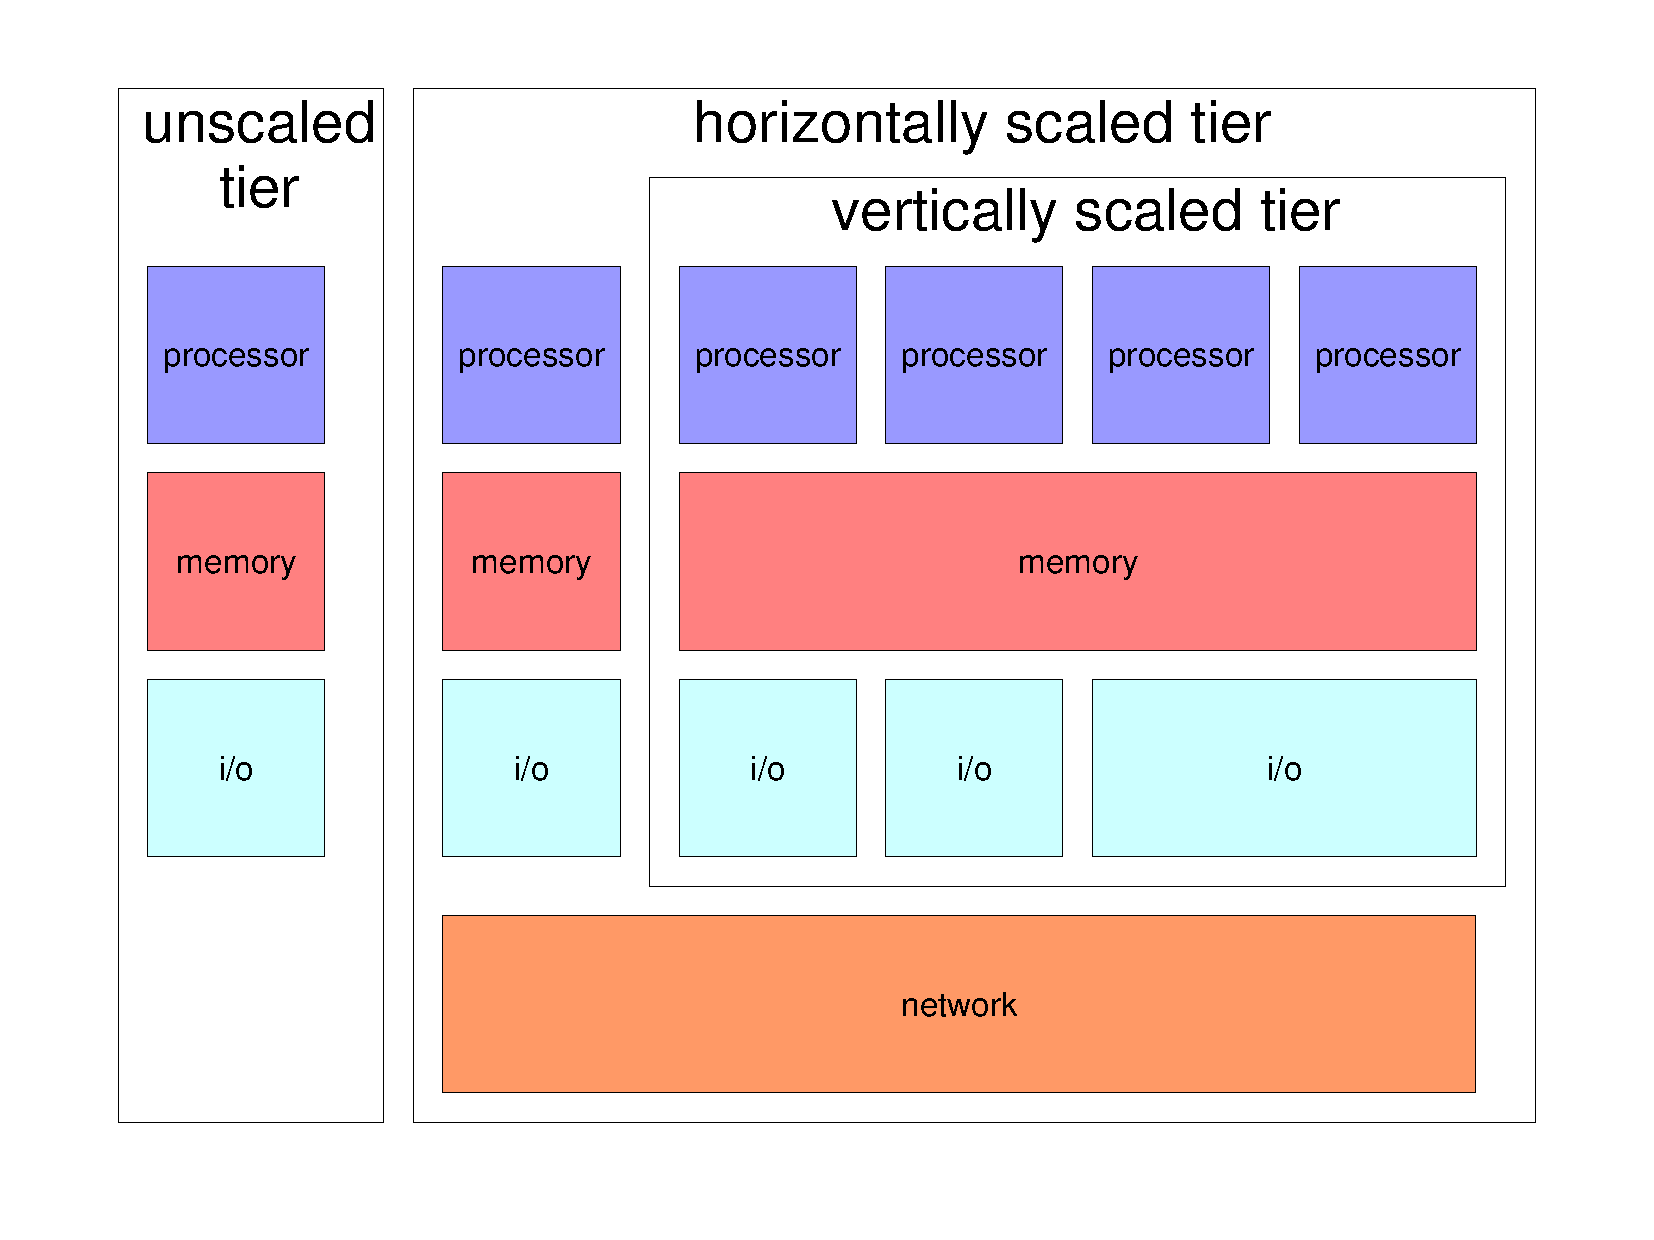
\includegraphics[scale=0.3,angle=-90]{graphic/scaling.pdf}
        \caption{Vertical and Horizontal Scaling}
        \label{scaling_figure}
    \end{center}
\end{figure}

Vertical servers are large \emph{Symmetric Multiprocessing} (SMP) systems with
more than four \emph{Central Processing Units} (CPU) that share one common memory.
One single \emph{Operating System} (OS) instance covers the processors, the memory
and input/ output (i/o) components. Vertical servers provide high availability by
building numerous \emph{Reliability, Availability, Serviceability} (RAS) features
into the individual server, to minimise un-/planned downtime.

The alternative horizontal scaling connects many systems over network, which is
often called \emph{Clustering}. A cluster contains computing nodes having one to
four processors and a memory each. The input/ output devices may belong to just
one node or be shared by many. Each node has an OS instance. \textit{Horizontal
servers do not build RAS features into the individual servers but get high RAS
by replication and deployment of many servers}, as Atwood \cite{atwood} writes.

\begin{table}[ht]
    \begin{center}
        \begin{footnotesize}
        \begin{tabular}{| p{50mm} | p{60mm} |}
            \hline
            \textbf{Vertical System} & \textbf{Horizontal System}\\
            \hline
            Large Database & Web Server\\
            \hline
            Transactional Database & Firewall\\
            \hline
            Data Warehouse & Proxy Server\\
            \hline
            Data Mining & Directories\\
            \hline
            Application Server & Application Server\\
            \hline
            High Performance Technical Computing (HPTC) application (non-partitionable) & High Performance Technical Computing (HPTC) application (partitionable)\\
            \hline
            & Media Streaming\\
            \hline
            & Extensible Markup Language (XML) Processing\\
            \hline
            & Java Server Pages (JSP) Application\\
            \hline
            & Secure Socket Layer (SSL)\\
            \hline
            & Virtual Private Network (VPN)\\
            \hline
        \end{tabular}
        \end{footnotesize}
        \caption{Vertical and Horizontal Application Types \cite{atwood}}
        \label{scalability_table}
    \end{center}
\end{table}

Table \ref{scalability_table} states some typical applications for vertical and
horizontal computing. The key difference, that after \cite{atwood} affected
both, their price and performance, is the \emph{Interconnect} used with each
architecture. Horizontal servers use a loosely-coupled \emph{external}
interconnect. Vertical servers use a tightly-coupled \emph{internal}
interconnect that makes data communications faster.

%
% $RCSfile$
%
% Copyright (c) 2005-2006. Christian Heller. All rights reserved.
%
% Permission is granted to copy, distribute and/or modify this document
% under the terms of the GNU Free Documentation License, Version 1.1 or
% any later version published by the Free Software Foundation; with no
% Invariant Sections, with no Front-Cover Texts and with no Back-Cover
% Texts. A copy of the license is included in the section entitled
% "GNU Free Documentation License".
%
% http://www.cybop.net
% - Cybernetics Oriented Programming -
%
% http://www.resmedicinae.org
% - Information in Medicine -
%
% Version: $Revision$ $Date$ $Author$
% Authors: Christian Heller <christian.heller@tuxtax.de>
%

\subsection{Misleading Tiers}
\label{misleading_tiers_heading}

When distinguishing human- and technical systems, the kinds of
\emph{Communication} are:

\begin{itemize}
    \item[-] Human $\leftrightarrow$ Human
    \item[-] Human $\leftrightarrow$ Computer
    \item[-] Computer $\leftrightarrow$ Computer
\end{itemize}

Each of these relies on different techniques, transport mechanisms, languages
(protocols) and so on. But the general principle after which communication
works, is always the same -- no matter whether technical \emph{Computer}
systems or their biological prototype, the \emph{Human Being}, are considered:
Information is \emph{received}, \emph{stored}, \emph{processed} and \emph{sent}.
Despite these common characteristics, today's \emph{Information Technology}
(IT) environments \cite{hellerkunze} treat communication between a computer
system and a human being differently than that \emph{among} computer systems.

\begin{figure}[ht]
    \begin{center}
        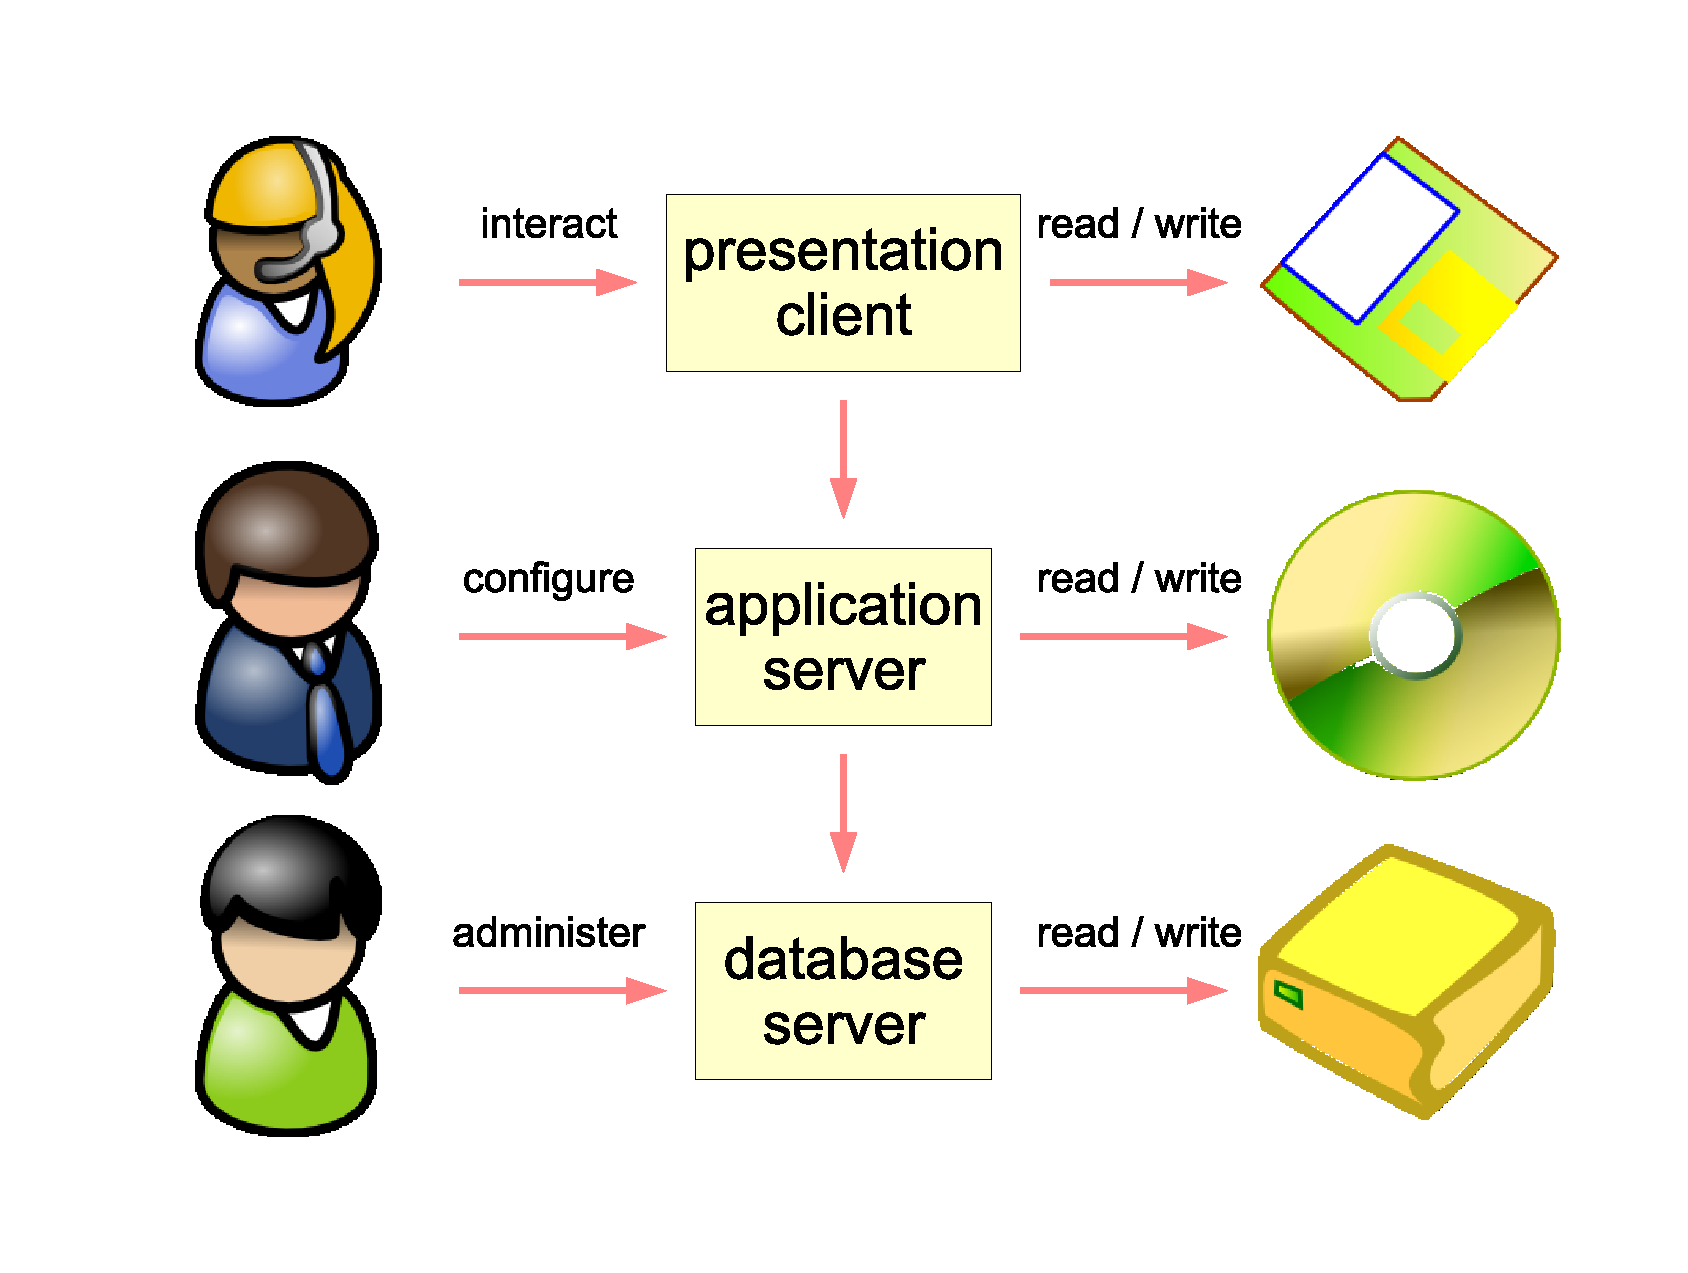
\includegraphics[scale=0.2]{vector/misleading.eps}
        \caption{Universal Communication}
        \label{misleading_figure}
    \end{center}
\end{figure}

Figure \ref{misleading_figure} shows a three-tier environment: tier 1 represents
the \emph{Presentation Layer}; tier 2 stands for the \emph{Application Layer};
tier 3 is the \emph{Database (DB) Layer}. Typical synonyms are, in this order:
\emph{Frontend}, \emph{Business Logic} and \emph{Backend}. The tiers (layers)
serve two needs: connect different locations and share work load (\emph{Scaling}).
However, the split into tiers of that kind raises two illusions:

\begin{enumerate}
    \item \emph{Users only interact with clients}
    \item \emph{Persistent data are stored in DB only}
\end{enumerate}

Many IT architectures, or at least their illustrations, neglect the fact that
in reality \emph{all} systems need a \emph{User Interface} (UI), for at least
being administered by humans, and \emph{almost} all systems, even
\emph{Database Management Systems} (DBMS) themselves, store some of their
persistent data outside a database, for example locally available configuration
information. This is not necessarily a problem for the IT environment as such,
but it is for the internal architecture of software systems. Special solutions
have to deal with frontend (UI framework), business logic (domain patterns) and
backend (data mapping), and often additional mechanisms for local and remote
communication. The serious differences in these design solutions are one root
of well-known problems like multi- directional inter-dependencies between system
parts, that make software difficult to develop and hard to maintain.

One aim of the work described in this article was to investigate possibilities
for a \emph{unification} of communication paradigms, that is high-level design
paradigms rather than low-level protocols, in order to architect software in a
way that allows the computer system it runs on to communicate \emph{universally}.


\newpage{\pagestyle{empty}\cleardoublepage}
%
% $RCSfile: logical_architecture.tex,v $
%
% Copyright (c) 2001-2004. Christian Heller. All rights reserved.
%
% No copying, altering, distribution or any other actions concerning this
% document, except after explicit permission by the author!
% At some later point in time, this document is planned to be put under
% the GNU FDL license. For now, _everything_ is _restricted_ by the author.
%
% http://www.cybop.net
% - Cybernetics Oriented Programming -
%
% http://www.resmedicinae.org
% - Information in Medicine -
%
% @author Christian Heller <christian.heller@tuxtax.de>
%

\section{Logical Architecture}
\label{logical_architecture_heading}

This section will sort the design patterns of section \ref{basic_patterns_heading}
into the layered architecture of a standard application. Afterwards, the
hierarchical principles of section \ref{hierarchy_and_ontology_heading} are applied
to simplify and merge the design patterns which will lead to an ontology.

\begin{figure}[ht]
    \begin{center}
        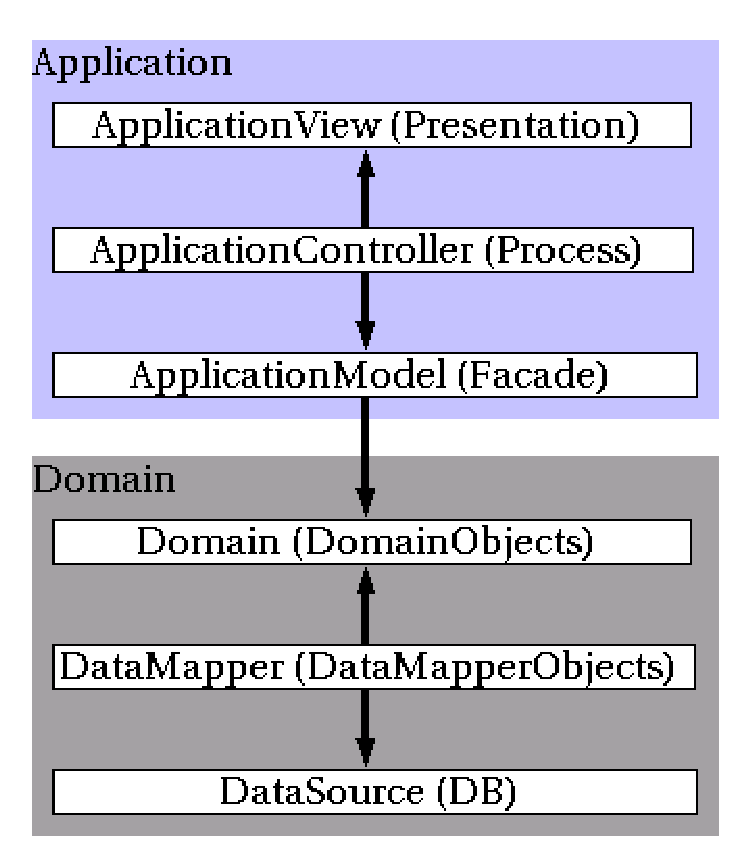
\includegraphics[scale=0.3]{vector/layered_architecture.eps}
        \caption{Layered Architecture}
        \label{layered_architecture_figure}
    \end{center}
\end{figure}

A state-of-the-art software system consists of a layered architecture similar to the
one shown in figure \ref{layered_architecture_figure}. The startable \emph{Controller}
process creates the whole application tree, to which belong the \emph{View} (as
user interface), the \emph{Model} (providing data to the view and as facade to
remote servers) and the \emph{Domain} with its database \emph{Mapper} layer.\\
It is not difficult to figure out where the basic patterns of section \ref{basic_patterns_heading}
fit in here (figure \ref{layered_architecture_with_basic_patterns_figure}):
The \emph{Model View Controller} pattern determines the classes to interact with
a human user via the \emph{View} (sometimes called \emph{Presentation Layer});
the \emph{Data Mapper} pattern provides necessary classes and an \emph{Entity
Relationship Model} (ERM) to connect to a persistence medium such as a database;
the \emph{Data Transfer Object} (DTO) pattern, finally, serves as means of
communication with remote servers.

\begin{figure}[ht]
    \begin{center}
        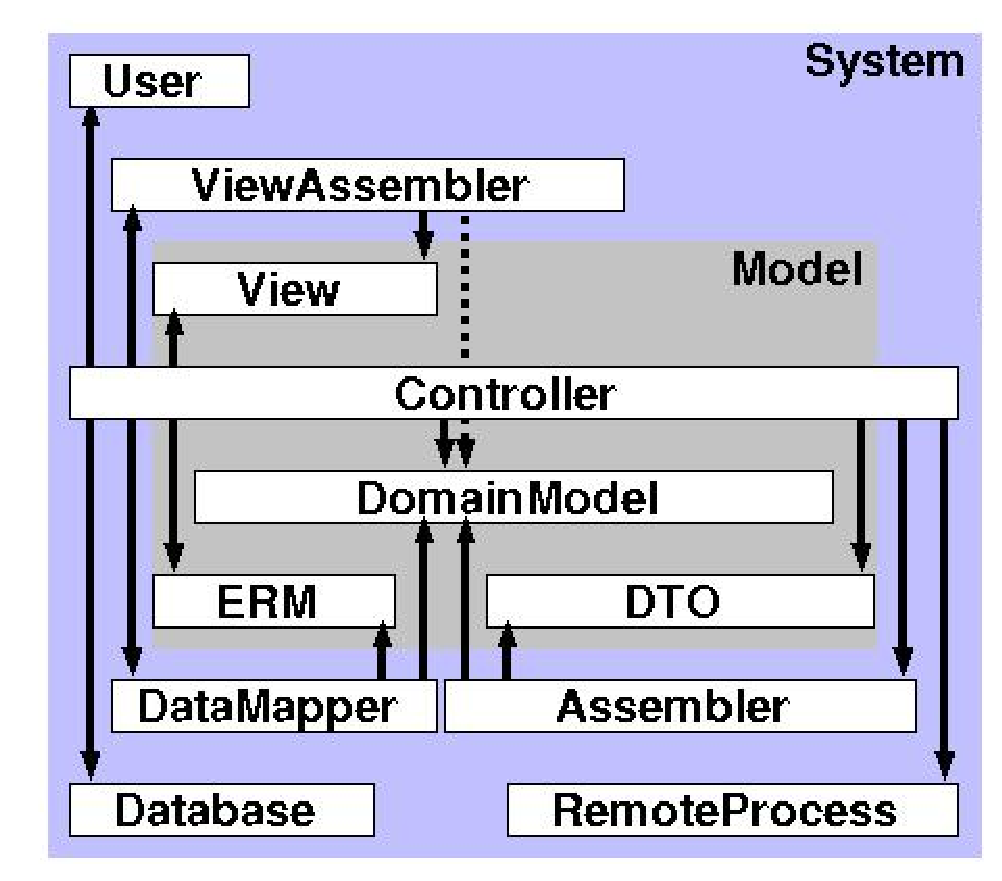
\includegraphics[scale=0.3]{vector/layered_architecture_with_basic_patterns.eps}
        \caption{Layered Architecture with Basic Patterns}
        \label{layered_architecture_with_basic_patterns_figure}
    \end{center}
\end{figure}

For all three kinds of communication, there is a:
\begin{itemize}
    \item[-] System (HumanUser, DataBase, RemoteServer)
    \item[-] Model (View, ERM, DTO)
    \item[-] Translator (ViewAssembler, Mapper, DTOAssembler)
\end{itemize}

Realizing this, it is easy to create ontological layers by adding one common
parent class for systems, models and translators each, which leads to a much
clearer architecture (figure \ref{layered_architecture_with_merged_patterns_figure}).
The common properties of all sub classes are merged into their corresponding super
class.

\begin{figure}[ht]
    \begin{center}
        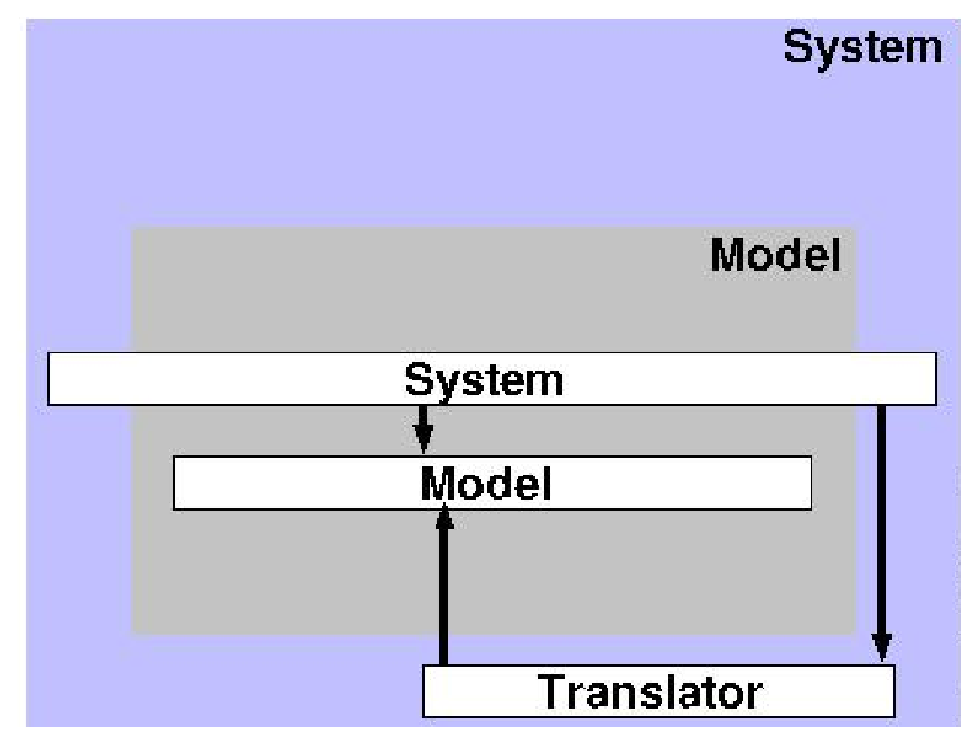
\includegraphics[scale=0.3]{vector/layered_architecture_with_merged_patterns.eps}
        \caption{Layered Architecture with merged Patterns}
        \label{layered_architecture_with_merged_patterns_figure}
    \end{center}
\end{figure}


\newpage{\pagestyle{empty}\cleardoublepage}
%
% $RCSfile: extended_motivation.tex,v $
%
% Copyright (C) 2002-2008. Christian Heller.
%
% Permission is granted to copy, distribute and/or modify this document
% under the terms of the GNU Free Documentation License, Version 1.1 or
% any later version published by the Free Software Foundation; with no
% Invariant Sections, with no Front-Cover Texts and with no Back-Cover
% Texts. A copy of the license is included in the section entitled
% "GNU Free Documentation License".
%
% http://www.cybop.net
% - Cybernetics Oriented Programming -
%
% http://www.resmedicinae.org
% - Information in Medicine -
%
% Version: $Revision: 1.1 $ $Date: 2008-08-19 20:41:06 $ $Author: christian $
% Authors: Christian Heller <christian.heller@tuxtax.de>
%

\chapter{Extended Motivation}
\label{extended_motivation_heading}

\begin{flushright}
    \textsl{
        Those who don't have Courage to dream,\\
        will not have Power to fight.
    }\\
    \textsc{African Saying}
\end{flushright}

The previous chapters of part \ref{basics_heading} of this document investigated
state-of-the-art concepts for the development, physical- and logical architecture
of software, and some of their good and bad sides. The \emph{Suitability} of these
concepts for solving a problem, of course, heavily depends upon the intended area
of usage. This chapter introduces a new idea to software system design that is
as simple as it is helpful. It suggests to:

\begin{center}
    \textbf{Inspect solutions of various other disciplines of science,\\
    phenomenons of nature,\\
    and apply them to software engineering\\
    \ldots\ in order to find out if existing weaknesses can be eliminated.}
\end{center}

Taken as \emph{Extended Motivation} for this work, the idea leads to a new
perspective, from which traditional concepts appear in a very different light.
Former \emph{Strengths} (like the bundling of attributes and methods in an OOP
class) may suddenly be considered a \emph{Weakness}. Additionally, completely
\emph{New Conceptual Solutions} (like the unification of system communication
patterns) become possible. The merger of both, traditional and new concepts
results in the \emph{Cybernetics Oriented Programming} (CYBOP), as defined in
chapter \ref{introduction_heading}.

A description of the intended \emph{Approach} for applying
\emph{inter-disciplinary} concepts to software system design finalises this
chapter. Three topics that crystallise out here are \emph{Statics and Dynamics},
\emph{Knowledge Schema} and \emph{State and Logic}. They are explained together
with their parallels to science or nature in part \ref{contribution_heading}
following afterwards, which represents the actual \emph{Core} of this document.

%
% $RCSfile: idea.tex,v $
%
% Copyright (C) 2002-2008. Christian Heller.
%
% Permission is granted to copy, distribute and/or modify this document
% under the terms of the GNU Free Documentation License, Version 1.1 or
% any later version published by the Free Software Foundation; with no
% Invariant Sections, with no Front-Cover Texts and with no Back-Cover
% Texts. A copy of the license is included in the section entitled
% "GNU Free Documentation License".
%
% http://www.cybop.net
% - Cybernetics Oriented Programming -
%
% http://www.resmedicinae.org
% - Information in Medicine -
%
% Version: $Revision: 1.1 $ $Date: 2008-08-19 20:41:07 $ $Author: christian $
% Authors: Christian Heller <christian.heller@tuxtax.de>
%

\section{Idea}
\label{idea_heading}

Researchers quite often follow the approach of first looking into what nature
offers and then trying to engineer a similar solution. All kinds of tools and
machines were created this way, even (and most obviously, with respect to the
human body and mind) robots and computers. Some scientists take the principles
of human awareness as physical model to explain the \emph{Universe} \cite{ripota}.
Some business people and consultants see analogies between processes in the
human brain and \emph{Organisational Structures of a Company} \cite{schoenhofer}.
Researchers in human sciences systematise \emph{International Public Law} by
sharing it into the three parts \emph{Society}, \emph{Cooperation} and
\emph{Conflicts} which are chosen in analogy to biology, that is \emph{Anatomy},
\emph{Physiology} and \emph{Pathology} of international relations \cite{bierzanek}.

Considering all that, one question is at hand: \textit{Why not apply a similar
approach to software engineering?} If computers are built after the model of
the human being (information input, memorising, processing and output), why not
structure the software that actually \emph{runs} those computers after similar
models? It seems logical and clear, yet the reality looks different. This work
wants to change that, and thereby help to improve application programming.

In search for new concepts to structure software, other sciences are called in.
The idea to marry systems sciences (notably general systems theory and cybernetics)
for analysis with creative problem solving techniques of designers for synthesis
is not new. Swift \cite{designmatrix} for example tried to apply both in form of
\emph{Cyberpatterns} to complex systems problems, using a pattern language. Yet
while Swift had turned his attention to what he calls \textit{the extreme front
end}, this work goes one step further. It applies the principles of nature
(results of many different sciences) not only to the \emph{User Interface}
(frontend) of an application, but to whole software system architectures.

\begin{figure}[ht]
    \begin{center}
        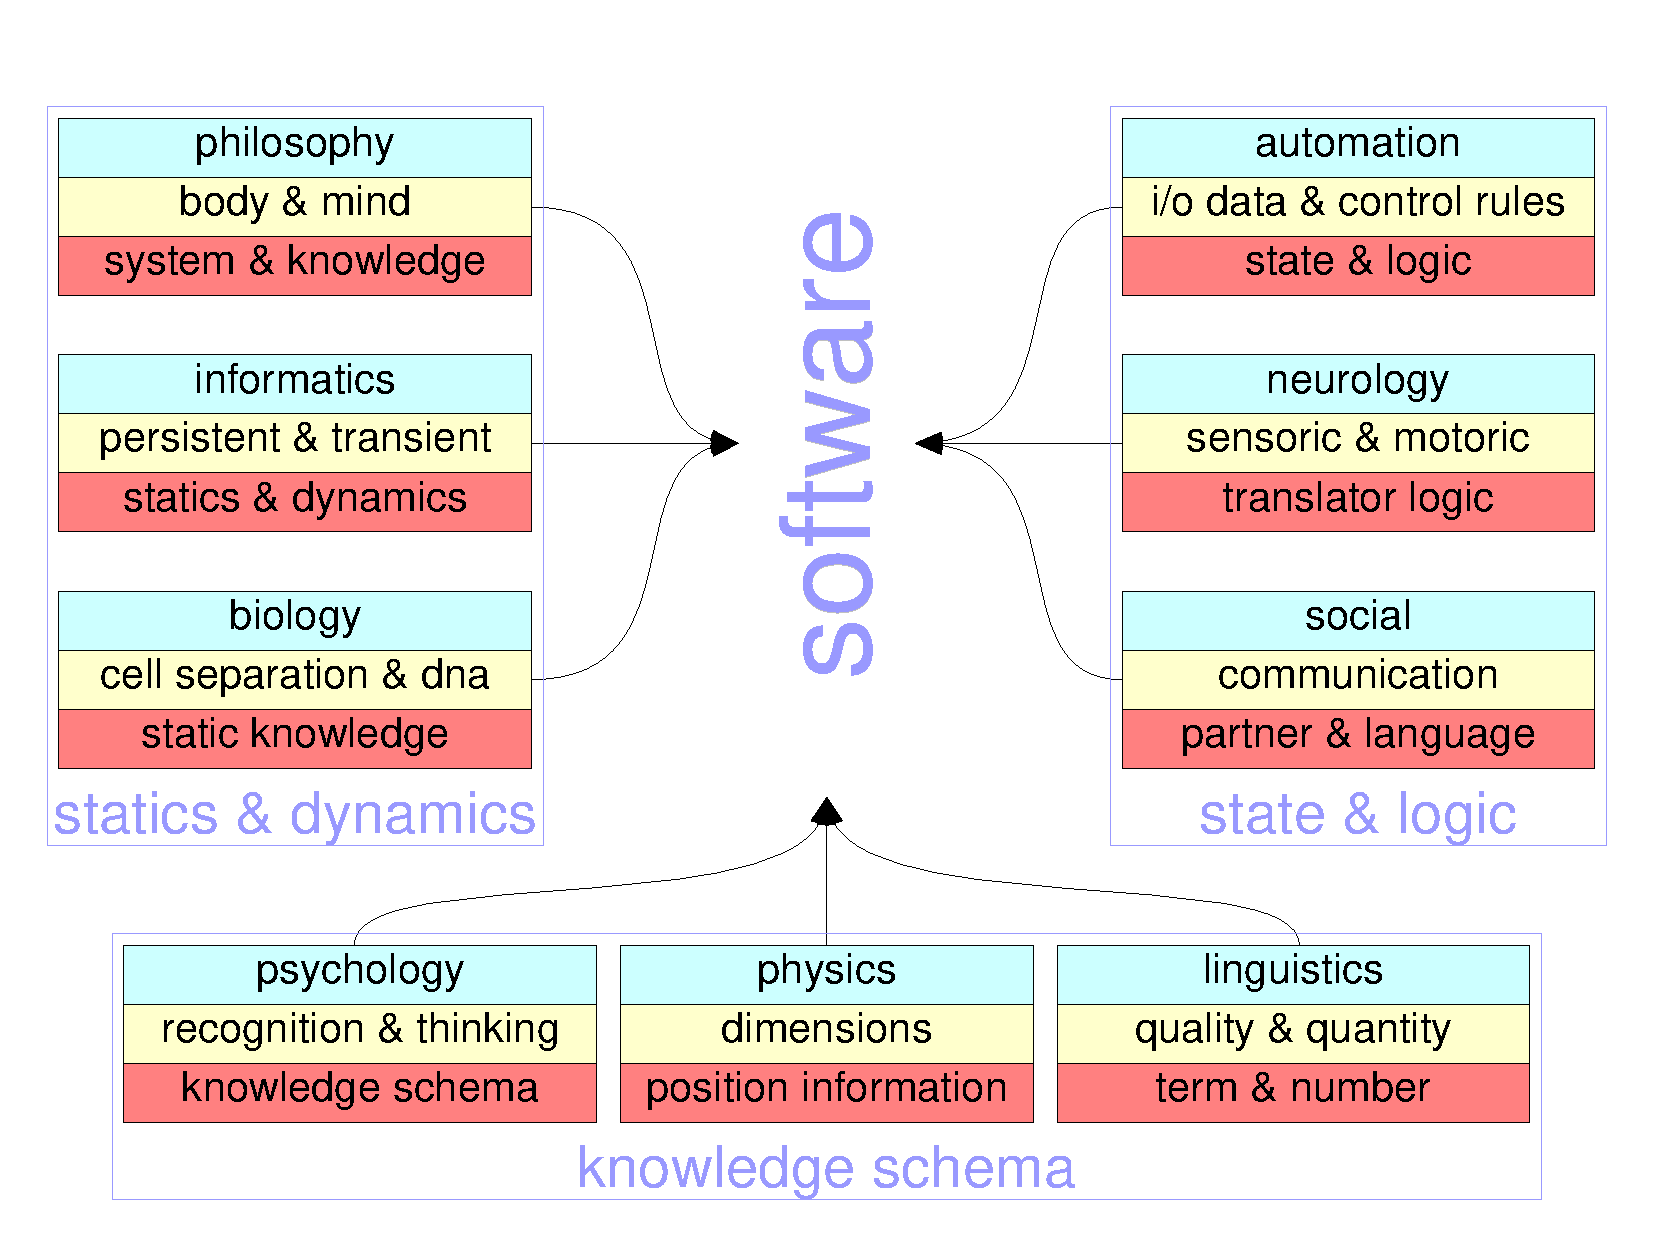
\includegraphics[scale=0.3,angle=-90]{graphic/mindmap.pdf}
        \caption{Mindmap of Sciences whose Principles influenced CYBOP}
        \label{mindmap_figure}
    \end{center}
\end{figure}

Figure \ref{mindmap_figure} shows some of the sciences whose principles were
considered in this work. The name of a field of science is shown on top of each
box. Made observations are mentioned below, in the middle. The resulting design
recommendations for software can be found at the bottom of each box. The
recommendations are grouped into those that justify a separation of
\emph{Statics and Dynamics} (left-hand side), a new kind of
\emph{Knowledge Schema} (lower part of the figure) and a distinction between
\emph{State and Logic} models (right-hand side).

It has to be mentioned though, that only some of the principles underlying a
specific field of science were considered in the figure and in more detail
later in this work. The figure does by no means claim to be complete. The shown
observations are only those that seemed promising in the context of software
design. The existence of persistent and transient data, for example, is only
one of many aspects of the science of informatics. Similarly is the existence
of sensoric and motoric nerve system just one aspect of the field of neurology.
And so on. Further details on the mentioned sciences and observations are not
given here, since later chapters will elaborate on them.

%
% $RCSfile: recapitulation.tex,v $
%
% Copyright (C) 2002-2008. Christian Heller.
%
% Permission is granted to copy, distribute and/or modify this document
% under the terms of the GNU Free Documentation License, Version 1.1 or
% any later version published by the Free Software Foundation; with no
% Invariant Sections, with no Front-Cover Texts and with no Back-Cover
% Texts. A copy of the license is included in the section entitled
% "GNU Free Documentation License".
%
% http://www.cybop.net
% - Cybernetics Oriented Programming -
%
% http://www.resmedicinae.org
% - Information in Medicine -
%
% Version: $Revision: 1.2 $ $Date: 2008-09-07 15:36:07 $ $Author: christian $
% Authors: Christian Heller <christian.heller@tuxtax.de>
%

\section{Recapitulation}
\label{recapitulation_heading}

The concepts that were found by considering other scientific disciplines, reveal
a number of state-of-the-art software design solutions that do not comply with
their original in nature, for example the:

\begin{enumerate}
    \item Mix of static application knowledge and instructions for dynamic
        system control (chapter \ref{statics_and_dynamics_heading})
    \item False combination of information ignoring hierarchical structure and
        mixing in meta information (chapter \ref{knowledge_schema_heading})
    \item Bundling of state- and logic knowledge (chapter
        \ref{state_and_logic_heading})
\end{enumerate}

\newpage

These discrepancies are the major reason for the issues mentioned in section
\ref{motivation_heading}. They become clearer only later in this work (part
\ref{contribution_heading}), where more background knowledge will be provided.
Almost all problems they cause have their root in \emph{Dependencies}. As a
system grows, the inter-dependencies between its single parts grow with. Why
does this happen? Simply because a clear architecture is missing. Even if
developers really try to follow a such -- on some point in the software's
lifetime, compromises have to be made due to unforeseen requirements and
dependencies:

\begin{itemize}
    \item[-] \emph{Meta Techniques} are used to provide basic functionality
    \item[-] \emph{Static Managers} accessible by any other parts in the system
        are introduced
    \item[-] \emph{Multiple Interfaces} are implemented to realise new
        properties (\emph{Mix-In})
    \item[-] \emph{Redundant Code} needs to be written to avoid too many
        unwanted inter-dependencies
    \item[-] \emph{Varying Mechanisms} are applied to plugin new software layers
\end{itemize}

It seems that today's software models rarely abstract the real world correctly.
This is \emph{not} general criticism on software development as it exists today,
\emph{nor} is it criticism on the abilities of application developers who use
current concepts and languages. It is just the neutral, unbiased realisation
that there are a few concepts in use which cause unclear, unnecessary, wrong
dependencies within software systems. The application of principles of other
scientific disciplines might have the potential to solve that.

It was early that, in the style of \emph{Bionics}, parallels between computing
machines and the human brain were seen, yet unfortunately do both not function
in exactly the same manner. Concepts like \emph{Artificial Neural Networks} (ANN)
%(section \ref{artificial_neural_networks_heading})
that try to imitate the
physical structure of the human brain exist, but are today's computers with
deterministic behaviour not built like that; they often have a
\emph{von Neumann Architecture} \cite{philippow}. This forces human programmers
to \emph{adapt} their thinking to the machine concepts.

Traditional programming languages and design solutions try to ease application
development by bridging the gap between concepts of human thinking and those of
the machine. Software developers are given tools to design programs in a more
abstract way, independently from the source code which gets generated later.
But as long as the underlying concepts of abstraction are insufficient, design
problems are to be expected. The kind and quality of abstractions is so
important, because it influences -- and \emph{is} influenced by -- all aspects
of software development (part \ref{basics_heading}) dealing with
\emph{Knowledge}:

\begin{itemize}
    \item[-] the \emph{Software Engineering Process} specifies static knowledge
        models (abstractions resulting from process phases), to be later
        dynamically processed in a computer system
    \item[-] the \emph{Physical Architecture} requires the translation of
        knowledge models (communication) between systems
    \item[-] the \emph{Logical Architecture} provides the means to represent
        knowledge models (by languages and various techniques) within a system
\end{itemize}

They all, consciously or not, are trials to apply human patterns. The structure
of knowledge models, for example, is based on concepts of \emph{Human Thinking},
the logical \emph{Mind} -- as opposed to the above-mentioned neural networks
that want to imitate the functioning of the physical \emph{Brain}. Because of
the central importance of knowledge, one aim of this work is to investigate new
techniques for its abstraction, to thereby revise state-of-the-art software
development. However, probably not all traditional concepts will be thrown
away. Basic things like control structures (looping, branching etc.)
abstracting logic knowledge in form of algorithms are still of importance but
appear in a different form (as will be shown in chapter
\ref{cybernetics_oriented_language_heading}). It therefore seems to be more
suitable to say that the new concepts will complement (and not revise
completely) existing development techniques, as was planned at the beginning of
this work (figure \ref{method_figure}).

%
% $RCSfile: approach.tex,v $
%
% Copyright (c) 2005-2006. Christian Heller. All rights reserved.
%
% Permission is granted to copy, distribute and/or modify this document
% under the terms of the GNU Free Documentation License, Version 1.1 or
% any later version published by the Free Software Foundation; with no
% Invariant Sections, with no Front-Cover Texts and with no Back-Cover
% Texts. A copy of the license is included in the section entitled
% "GNU Free Documentation License".
%
% http://www.cybop.net
% - Cybernetics Oriented Programming -
%
% http://www.resmedicinae.org
% - Information in Medicine -
%
% Version: $Revision: 1.1 $ $Date: 2006-01-03 08:21:45 $ $Author: christian $
% Authors: Christian Heller <christian.heller@tuxtax.de>
%

\section{Approach}
\label{approach_heading}

On its way to solving the issues mentioned in sections
\ref{introduction_heading} and \ref{architectural_troubles_heading}, the
work followed the \emph{Cybernetics Oriented Programming} (CYBOP) approach
\cite{heller2004}. The idea behind is as simple as it is helpful; it suggests
to:

\begin{center}
    Inspect solutions of various disciplines\\
    of science, phenomenons of nature,\\
    and apply them to software engineering.
\end{center}

Figure \ref{mindmap_figure} shows some sciences whose principles were
considered in this work. The name of a field of science is shown on top of each
box. Made observations are mentioned below, in the middle. The resulting design
recommendations for software can be found at the bottom of each box. The
recommendations are grouped into those that justify a distinction between
\emph{Statics and Dynamics}, a new kind of \emph{Knowledge Schema} and a
separation of \emph{State- and Logic} models.

\begin{figure}[ht]
    \begin{center}
        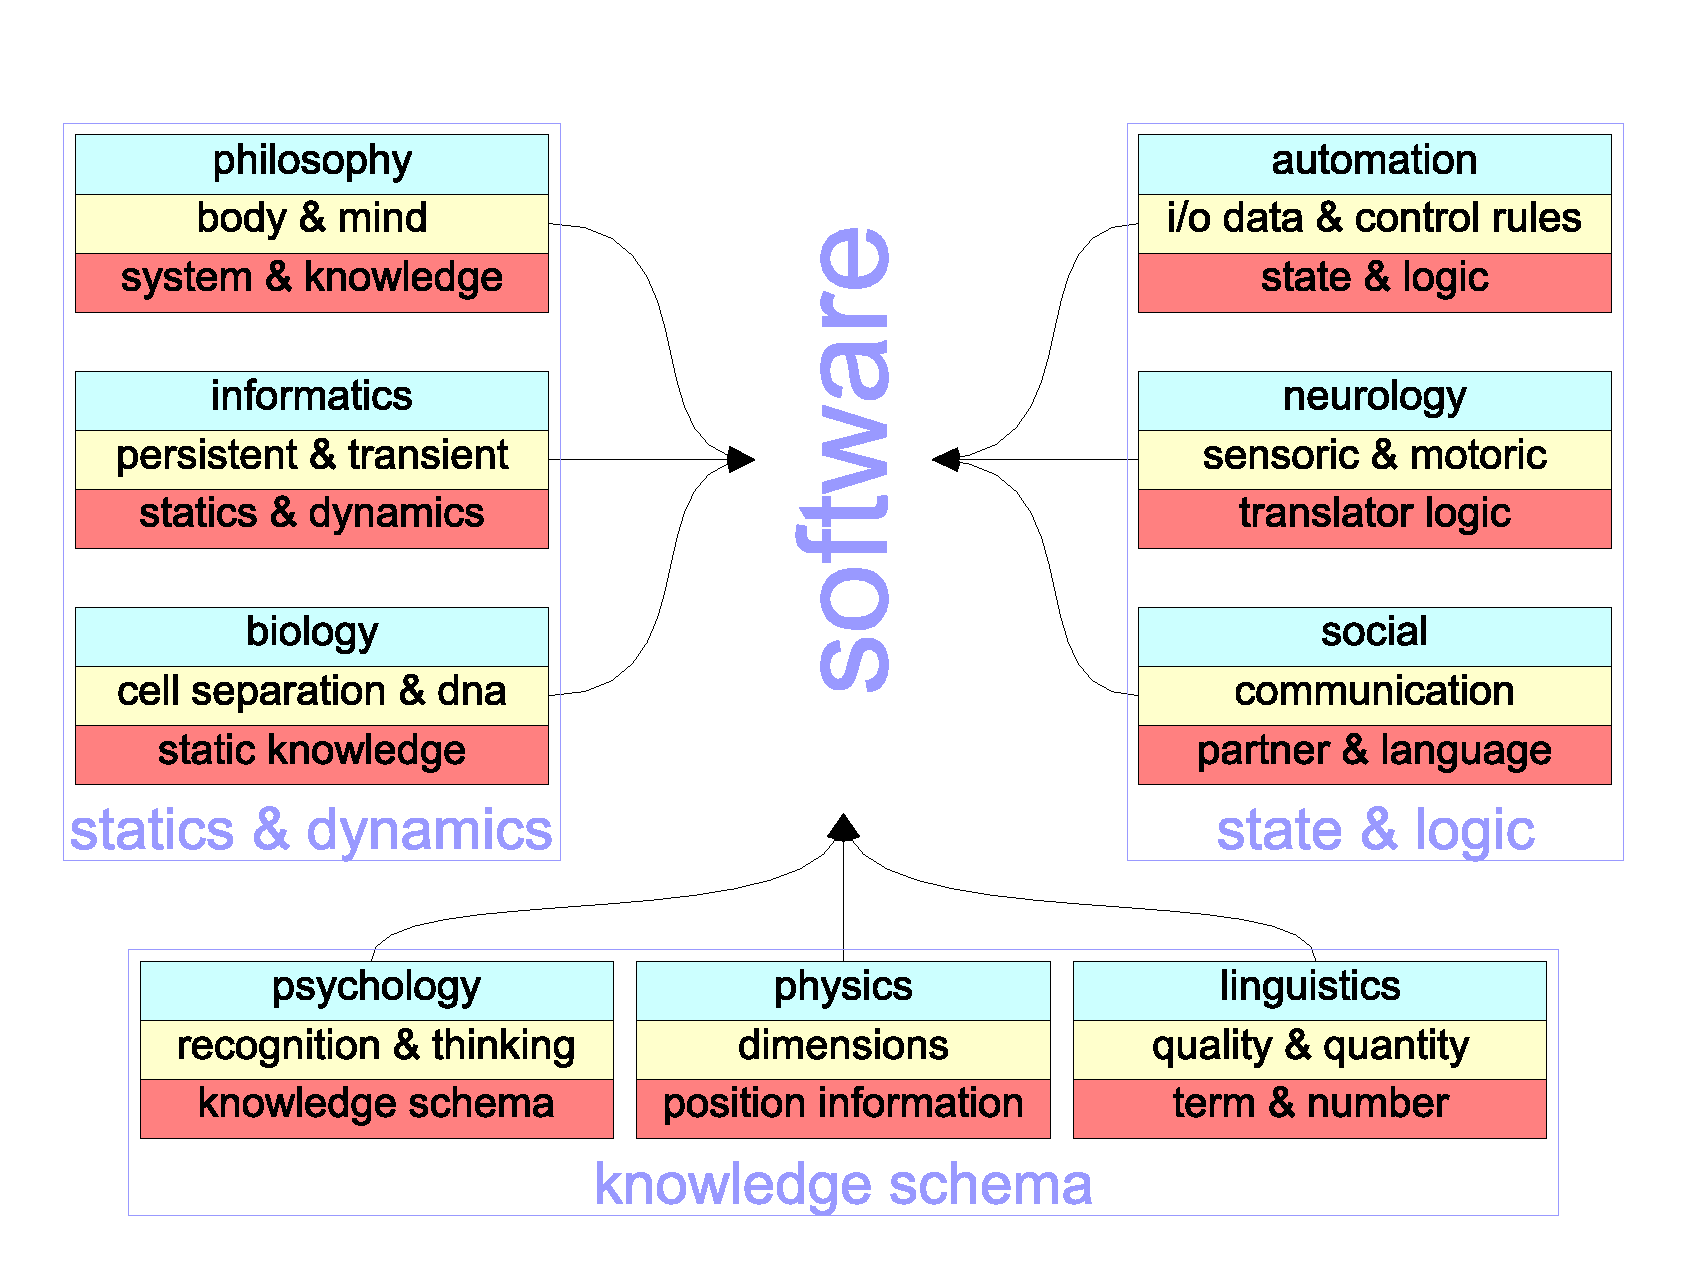
\includegraphics[scale=0.2]{vector/mindmap.eps}
        \caption{Mindmap of Influential Sciences}
        \label{mindmap_figure}
    \end{center}
\end{figure}

\begin{figure}[ht]
    \begin{center}
        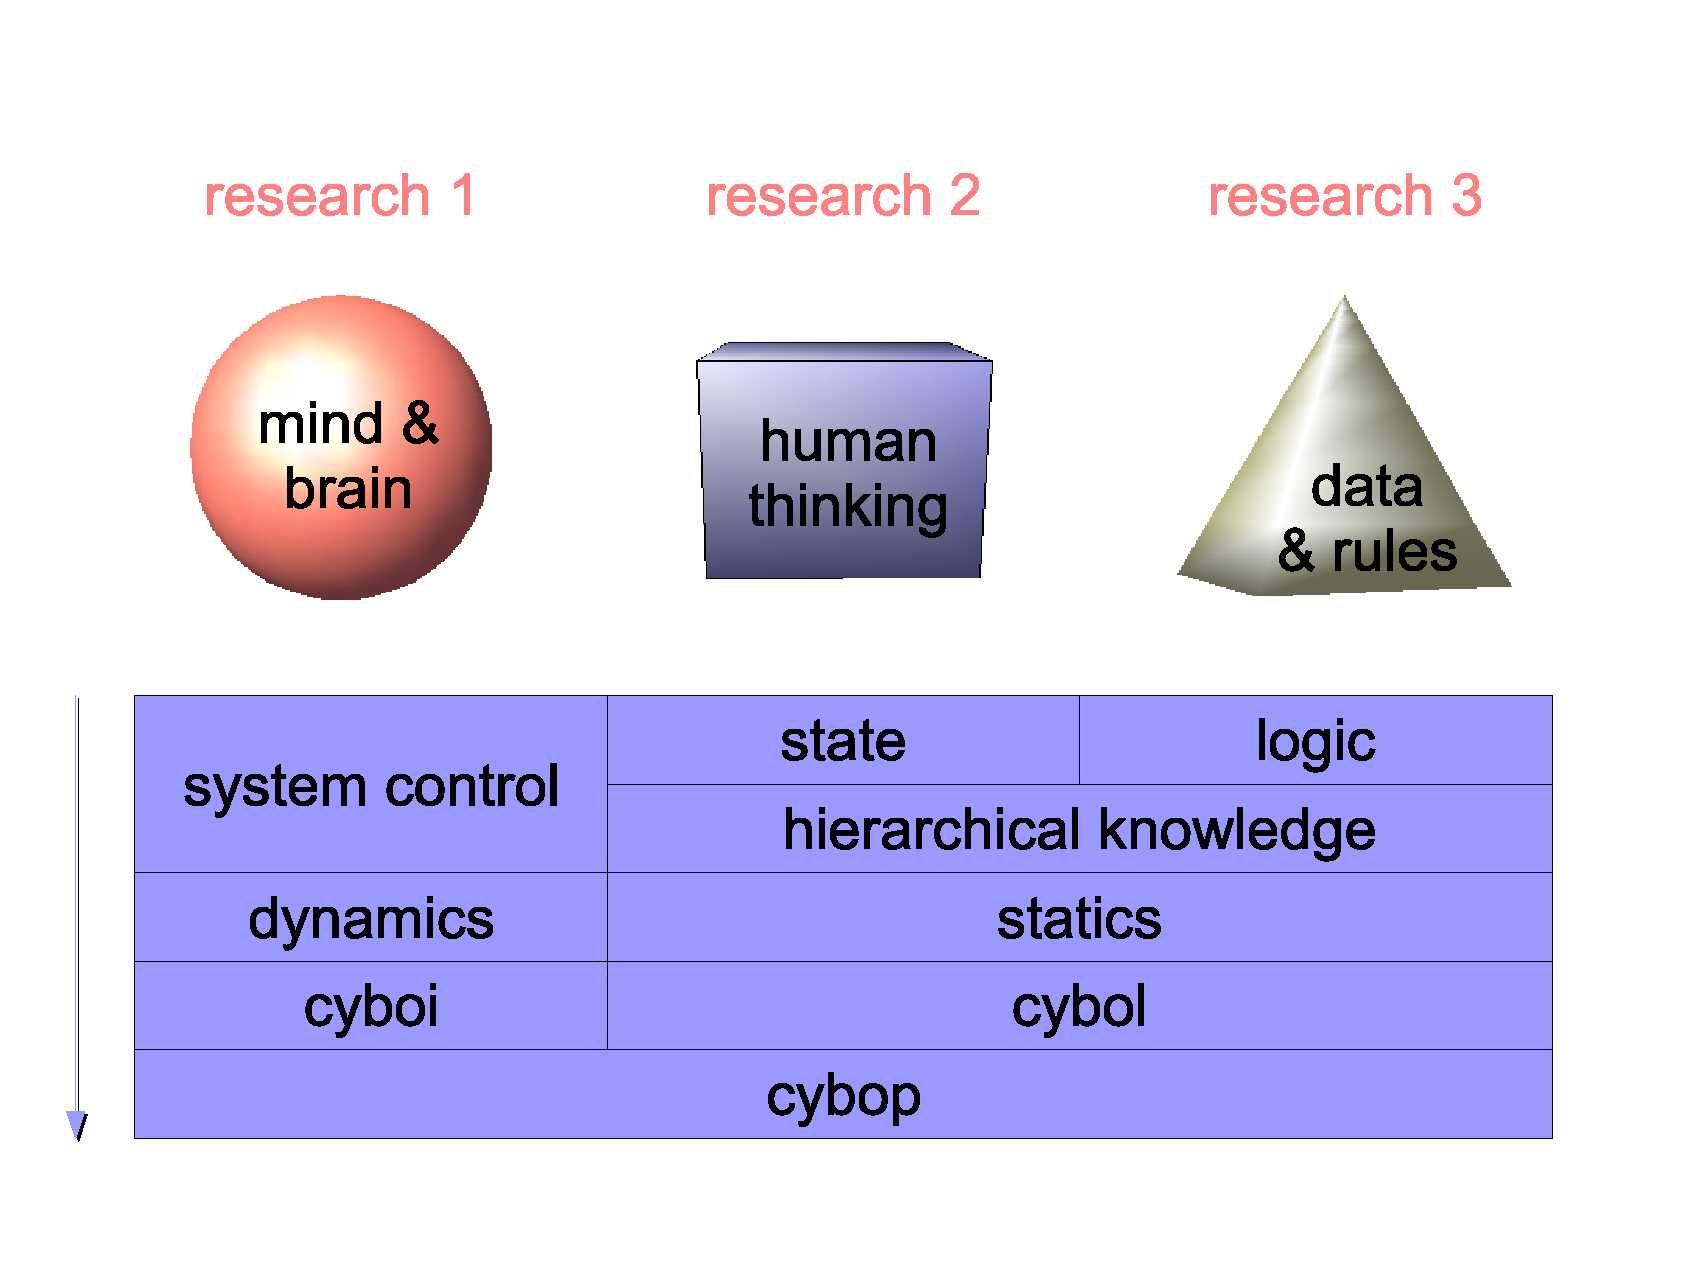
\includegraphics[scale=0.2]{vector/approach.eps}
        \caption{Overall CYBOP Approach}
        \label{approach_figure}
    \end{center}
\end{figure}

A first observation, when looking at human beings from a philosophical
perspective, is the separation of \emph{Mind} and \emph{Brain} (Body).
Accordingly, CYBOP treats computers as \emph{Systems} owning and processing
\emph{Knowledge}. This is not unlike the idea of \emph{Agent} systems owning a
\emph{Knowledge Base} \cite{parks, kuehnel}. All abstract knowledge that humans
make up belongs to their mind. The brain is merely a physical carrier of
knowledge. Similarly, there are actually two kinds of software: one
representing \emph{passive} knowledge and the other \emph{actively} controlling
a system's hardware.

Secondly, attention is payed to the concepts of \emph{Human Thinking}
\cite{heller2004}, as investigated by psychology. Through their application,
knowledge becomes \emph{hierarchical}. Moreover, this work tries to embed
knowledge models in an environment of \emph{Dimensions}, as known from physics.
Every model keeps a number of \emph{Meta Information} about its parts.
\emph{Positions} in space or time are one such example.

Thirdly, \emph{State-} gets distinguished from \emph{Logic} knowledge. It is
known from neurological research that the human brain has special communication
regions that, simply spoken, do nothing else than translating data, i.e. an
input- into an output \emph{State}, according to rules of \emph{Logic}. Systems
theory uses similar abstractions. When talking about states, this work means a
composed \emph{Set} of states.

In CYBOP (figure \ref{approach_figure}), all knowledge (states and logic),
belongs to a system's \emph{Statics}, and is described by CYBOL language
templates (section \ref{practical_proof_heading}). The processing of knowledge
at runtime, to control a system, is \emph{Dynamics} and happens in the CYBOI
interpreter.



    \newpage{\pagestyle{empty}\cleardoublepage}
    %
% $RCSfile: contribution.tex,v $
%
% Copyright (C) 2002-2008. Christian Heller.
%
% Permission is granted to copy, distribute and/or modify this document
% under the terms of the GNU Free Documentation License, Version 1.1 or
% any later version published by the Free Software Foundation; with no
% Invariant Sections, with no Front-Cover Texts and with no Back-Cover
% Texts. A copy of the license is included in the section entitled
% "GNU Free Documentation License".
%
% http://www.cybop.net
% - Cybernetics Oriented Programming -
%
% http://www.resmedicinae.org
% - Information in Medicine -
%
% Version: $Revision: 1.1 $ $Date: 2008-08-19 20:41:06 $ $Author: christian $
% Authors: Christian Heller <christian.heller@tuxtax.de>
%

\part{Contribution}
\label{contribution_heading}
\newpage{\pagestyle{empty}\cleardoublepage}

%
% $RCSfile: statics_and_dynamics.tex,v $
%
% Copyright (c) 2005-2006. Christian Heller. All rights reserved.
%
% Permission is granted to copy, distribute and/or modify this document
% under the terms of the GNU Free Documentation License, Version 1.1 or
% any later version published by the Free Software Foundation; with no
% Invariant Sections, with no Front-Cover Texts and with no Back-Cover
% Texts. A copy of the license is included in the section entitled
% "GNU Free Documentation License".
%
% http://www.cybop.net
% - Cybernetics Oriented Programming -
%
% http://www.resmedicinae.org
% - Information in Medicine -
%
% Version: $Revision: 1.1 $ $Date: 2006-01-03 08:21:45 $ $Author: christian $
% Authors: Christian Heller <christian.heller@tuxtax.de>
%

\subsection{Statics and Dynamics}
\label{statics_and_dynamics_heading}

Over the years, it has turned out to be helpful in software design, to separate
\emph{Domain Knowledge} from \emph{Application Functionality}. In
one-or-another form, the architectural\\software patterns \cite{heller2005}
\emph{Layers}, \emph{Domain Model} and \emph{Model View Controller} (MVC) all
suggest to apply this principle.

The \emph{Tools \& Materials} approach \cite{tandm}\\talks of \emph{active}
applications (tools) working on \emph{passive} domain data (material). And also
\emph{System Family Engineering} (section \ref{architectural_troubles_heading})
bases on a separate treatment of domain and application, in form of
\emph{Domain Engineering} (DE) and \emph{Application Engineering} (AE).

An often neglected fact of these approaches is that not only the domain, but
also the application contains important business knowledge (figure
\ref{separation_figure}). The \emph{User Interface} (UI), for example, is
tailored for a specific business domain. And the logic behind, if not
contained in the UI itself, is often put in a \emph{Controller} which belongs
to the application$-$, not the domain layer.

\begin{figure}[ht]
    \begin{center}
        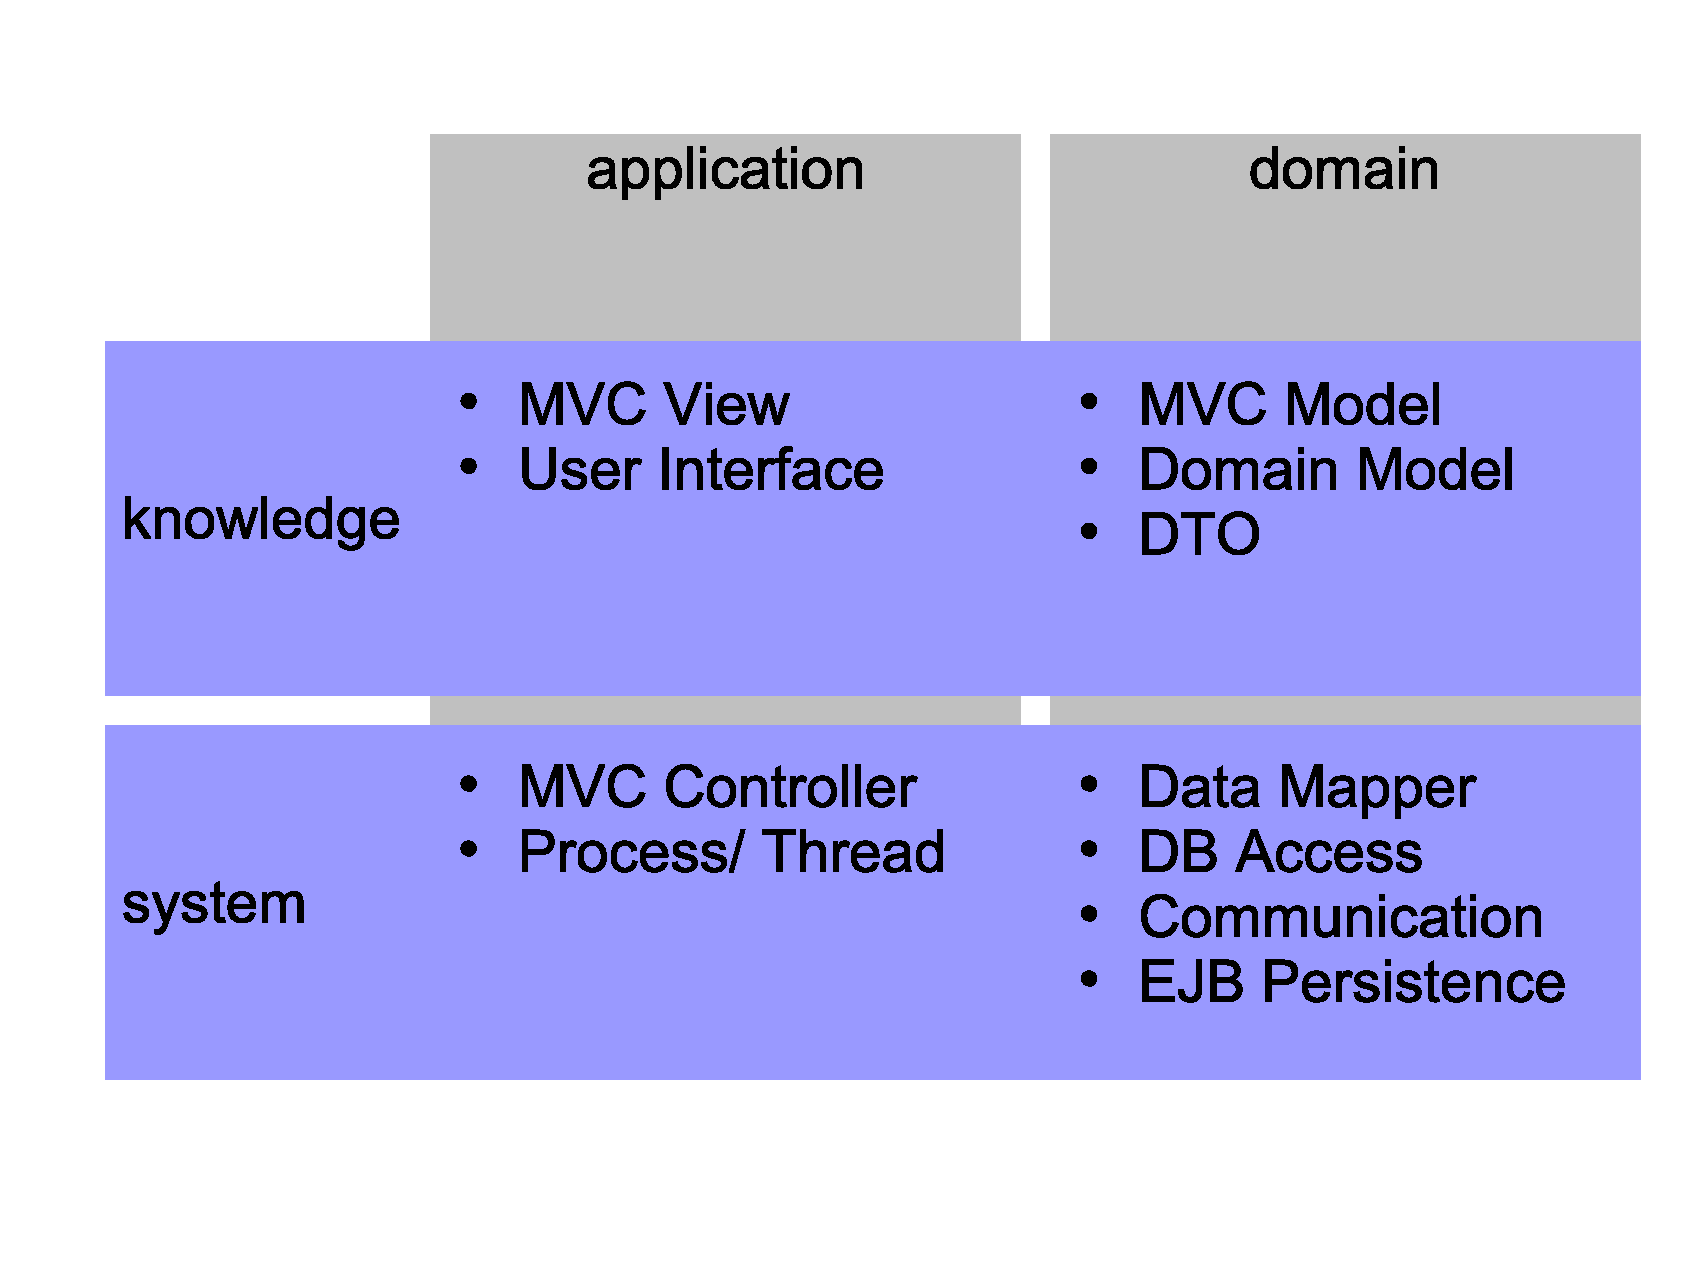
\includegraphics[scale=0.2]{vector/separation.eps}
        \caption{Different Knowledge Separations}
        \label{separation_figure}
    \end{center}
\end{figure}

Similarly, the domain often contains functionality which actually does belong
into the application process: \emph{Database} (DB) access is handled by help of
patterns like the \emph{Data Mapper} \cite{heller2005}, in which the mapper\\
objects contain \emph{Structured Query Language} (SQL) code to connect to a
\emph{Database Management System} (DBMS); \emph{Enterprise Java Beans} (EJB),
which should better be pure domain objects, imitate a \emph{Middleware}
providing persistence- or communication mechanisms, which originally have
nothing to do with the business knowledge they contain.

It is precisely this \emph{Mixup} of responsibilities between an application
system and its domain knowledge, that leads to multiple inter-dependencies and
hence unflexibility within a system. Instead, a separation should be made
between active \emph{System Control} and passive \emph{Knowledge}. A UI's
appearance would then be treated as domain knowledge, just as the logic of the
functions called through it. A data mapper would be transformed into a simple
\emph{Translator} -- similar to a \emph{Data Transfer Object} (DTO)
\cite{heller2005} -- that knows how to convert data from one domain model into
another; its DBMS access functionality, however, would be extracted and put
into the application system. Monstrosities like EJBs would likewise be opened
up and parted into their actual domain knowledge, and all other mechanisms
around -- the latter being moved into the application system.

To sum up this thought: The essential realisation here is that hardware-close
mechanisms like the ones necessary for data input/ output (i/o), enabling
inter-system communication, should be handled in an active application system
layer which was started as process on a computer, and \emph{not} be merged with
pure, passive domain knowledge. User interfaces and other data models which are
traditionally hold in the application layer, should rather belong to the domain
layer, together with all other business knowledge.

Now, if a distinction of high-level knowledge from low-level system control
software is considered to be useful, the next question must be: \textit{How,
that is in which form, best to store knowledge in a system?}

One possible structure called \emph{Data Garden} \cite{holland} was proposed by
Wau Holland of the \emph{Chaos Computer Club} (CCC). Although being a
non-academic organisation, his ideas on knowledge modelling are interesting to
this work. He dreamt of whole \emph{Forests}, \emph{Parks} or -- as the name
says -- \emph{Gardens} of \emph{Knowledge Trees} and \emph{Data Bushes} (figure
\ref{garden_figure}).

\begin{figure}[ht]
    \begin{center}
        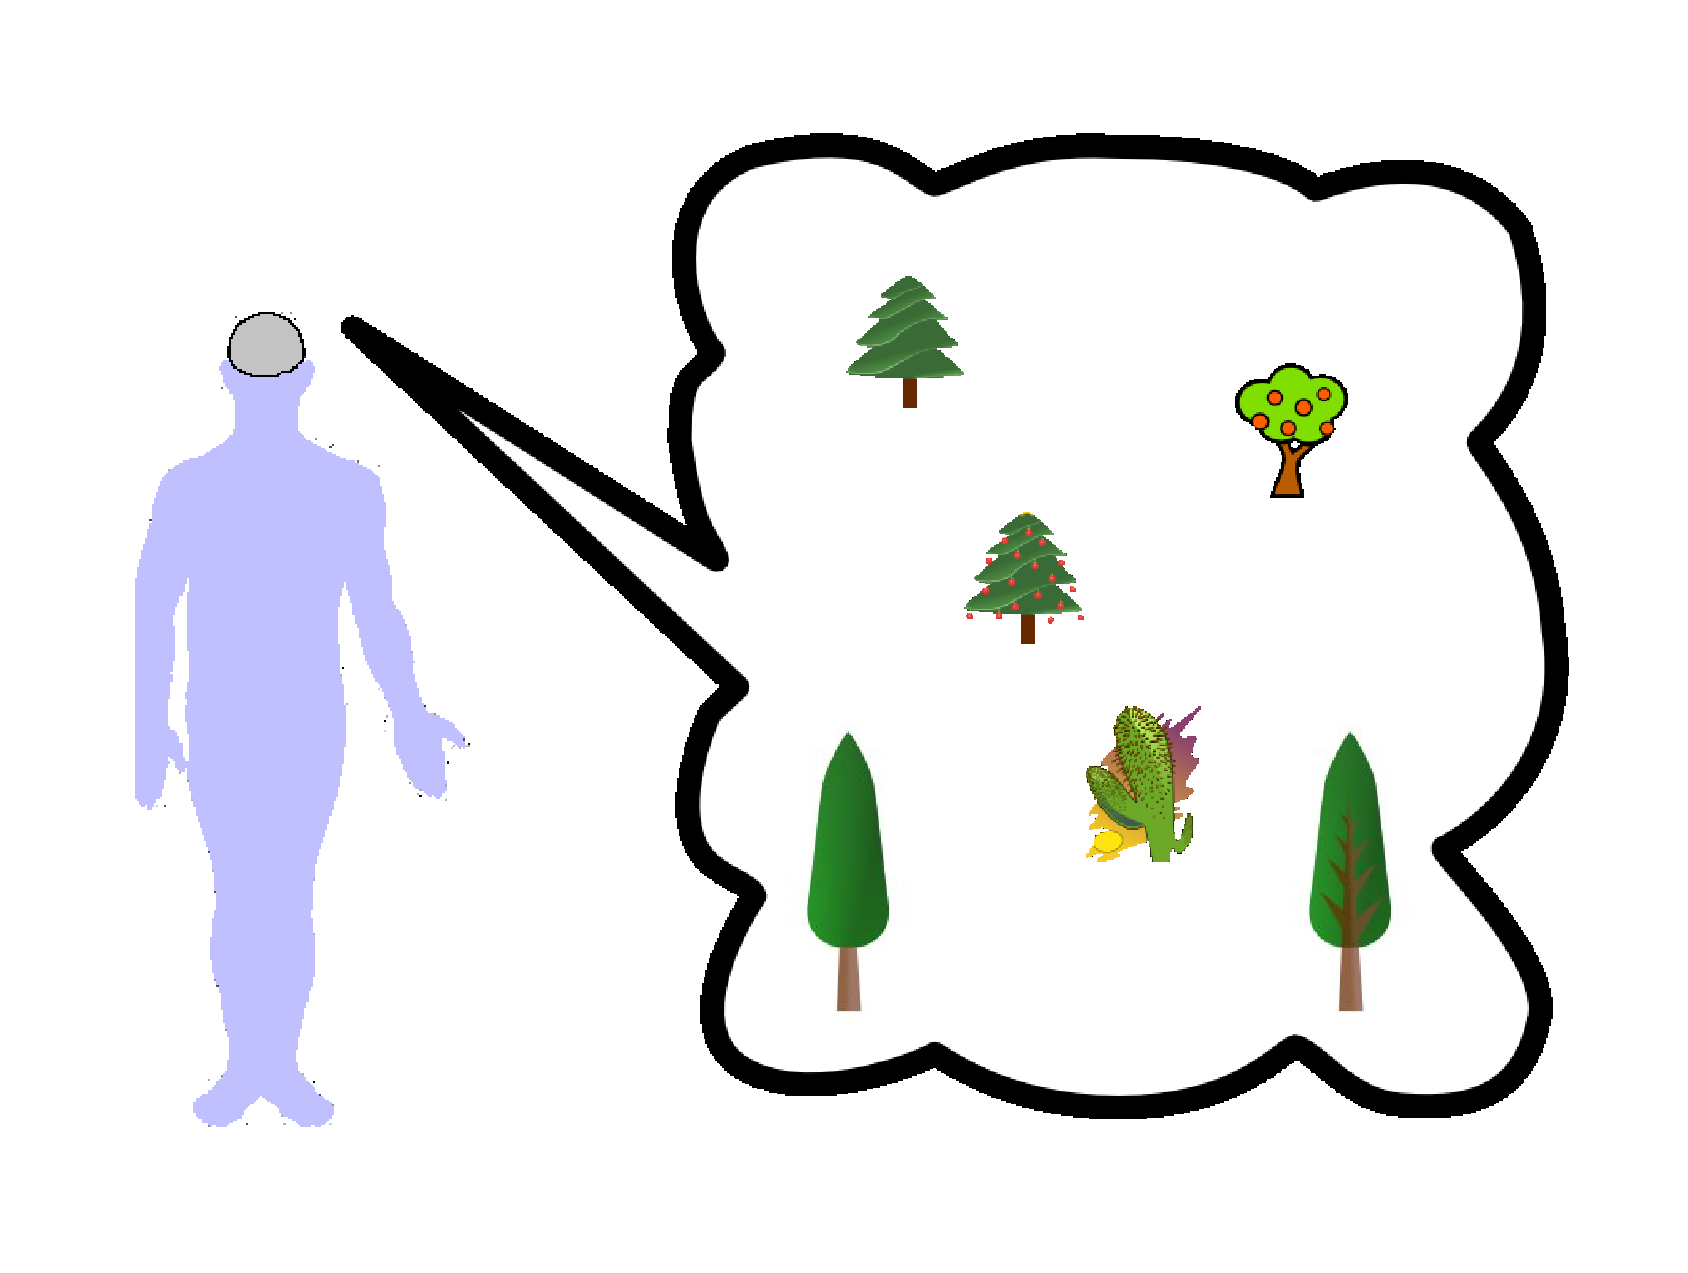
\includegraphics[scale=0.2]{vector/garden.eps}
        \caption{Data Garden}
        \label{garden_figure}
    \end{center}
\end{figure}

The interpreter created in the work described in this article stores all its
knowledge in \emph{one single} tree, whose root node it references. The single
concepts (data bushes) are represented by branches of that knowledge tree.

Further arguments in favour of a distinction of statics and dynamics are: mind
\& body (philosophy), cerebral cortex \& communication regions (neurology),
genetic information \& cell body (biology), long- \& short-term memory
(psychology), and more.

\newpage{\pagestyle{empty}\cleardoublepage}
%
% $RCSfile: knowledge_schema.tex,v $
%
% Copyright (c) 2005-2006. Christian Heller. All rights reserved.
%
% Permission is granted to copy, distribute and/or modify this document
% under the terms of the GNU Free Documentation License, Version 1.1 or
% any later version published by the Free Software Foundation; with no
% Invariant Sections, with no Front-Cover Texts and with no Back-Cover
% Texts. A copy of the license is included in the section entitled
% "GNU Free Documentation License".
%
% http://www.cybop.net
% - Cybernetics Oriented Programming -
%
% http://www.resmedicinae.org
% - Information in Medicine -
%
% Version: $Revision: 1.1 $ $Date: 2006-01-03 08:21:45 $ $Author: christian $
% Authors: Christian Heller <christian.heller@tuxtax.de>
%

\subsection{Knowledge Schema}
\label{knowledge_schema_heading}

Human beings have a brain which they use to think, in other words to build up a
mind. While the former exists in the \emph{Real World}, the latter is
constructed as a subjective \emph{Virtual World}. All people do think, all the
time, even not knowing that they do. One would therefore guess that the act of
\emph{Thinking} is a most common one, familiar to anybody. But judging from the
enormous research effort in sciences dealing with it, the \emph{Principles}
behind thinking are not that easy to grasp.

%
% $RCSfile: schema.tex,v $
%
% Copyright (c) 2005-2006. Christian Heller. All rights reserved.
%
% Permission is granted to copy, distribute and/or modify this document
% under the terms of the GNU Free Documentation License, Version 1.1 or
% any later version published by the Free Software Foundation; with no
% Invariant Sections, with no Front-Cover Texts and with no Back-Cover
% Texts. A copy of the license is included in the section entitled
% "GNU Free Documentation License".
%
% http://www.cybop.net
% - Cybernetics Oriented Programming -
%
% http://www.resmedicinae.org
% - Information in Medicine -
%
% Version: $Revision: 1.1 $ $Date: 2006-01-03 08:21:45 $ $Author: christian $
% Authors: Christian Heller <christian.heller@tuxtax.de>
%

\subsubsection{Schema}
\label{schema_heading}

A theoretical \emph{Model} is an abstract clip of the real world, and exists in
the human mind. Another common word for \emph{Model} is \emph{Concept}. It is
the subsumption of \emph{Item}, \emph{Category} and \emph{Compound}, resulting
from three activities of abstraction: \emph{Discrimination},
\emph{Categorisation} and \emph{Composition} \cite{heller2004}. Each model
\emph{knows} about the parts it consists of.

\begin{figure}[ht]
    \begin{center}
        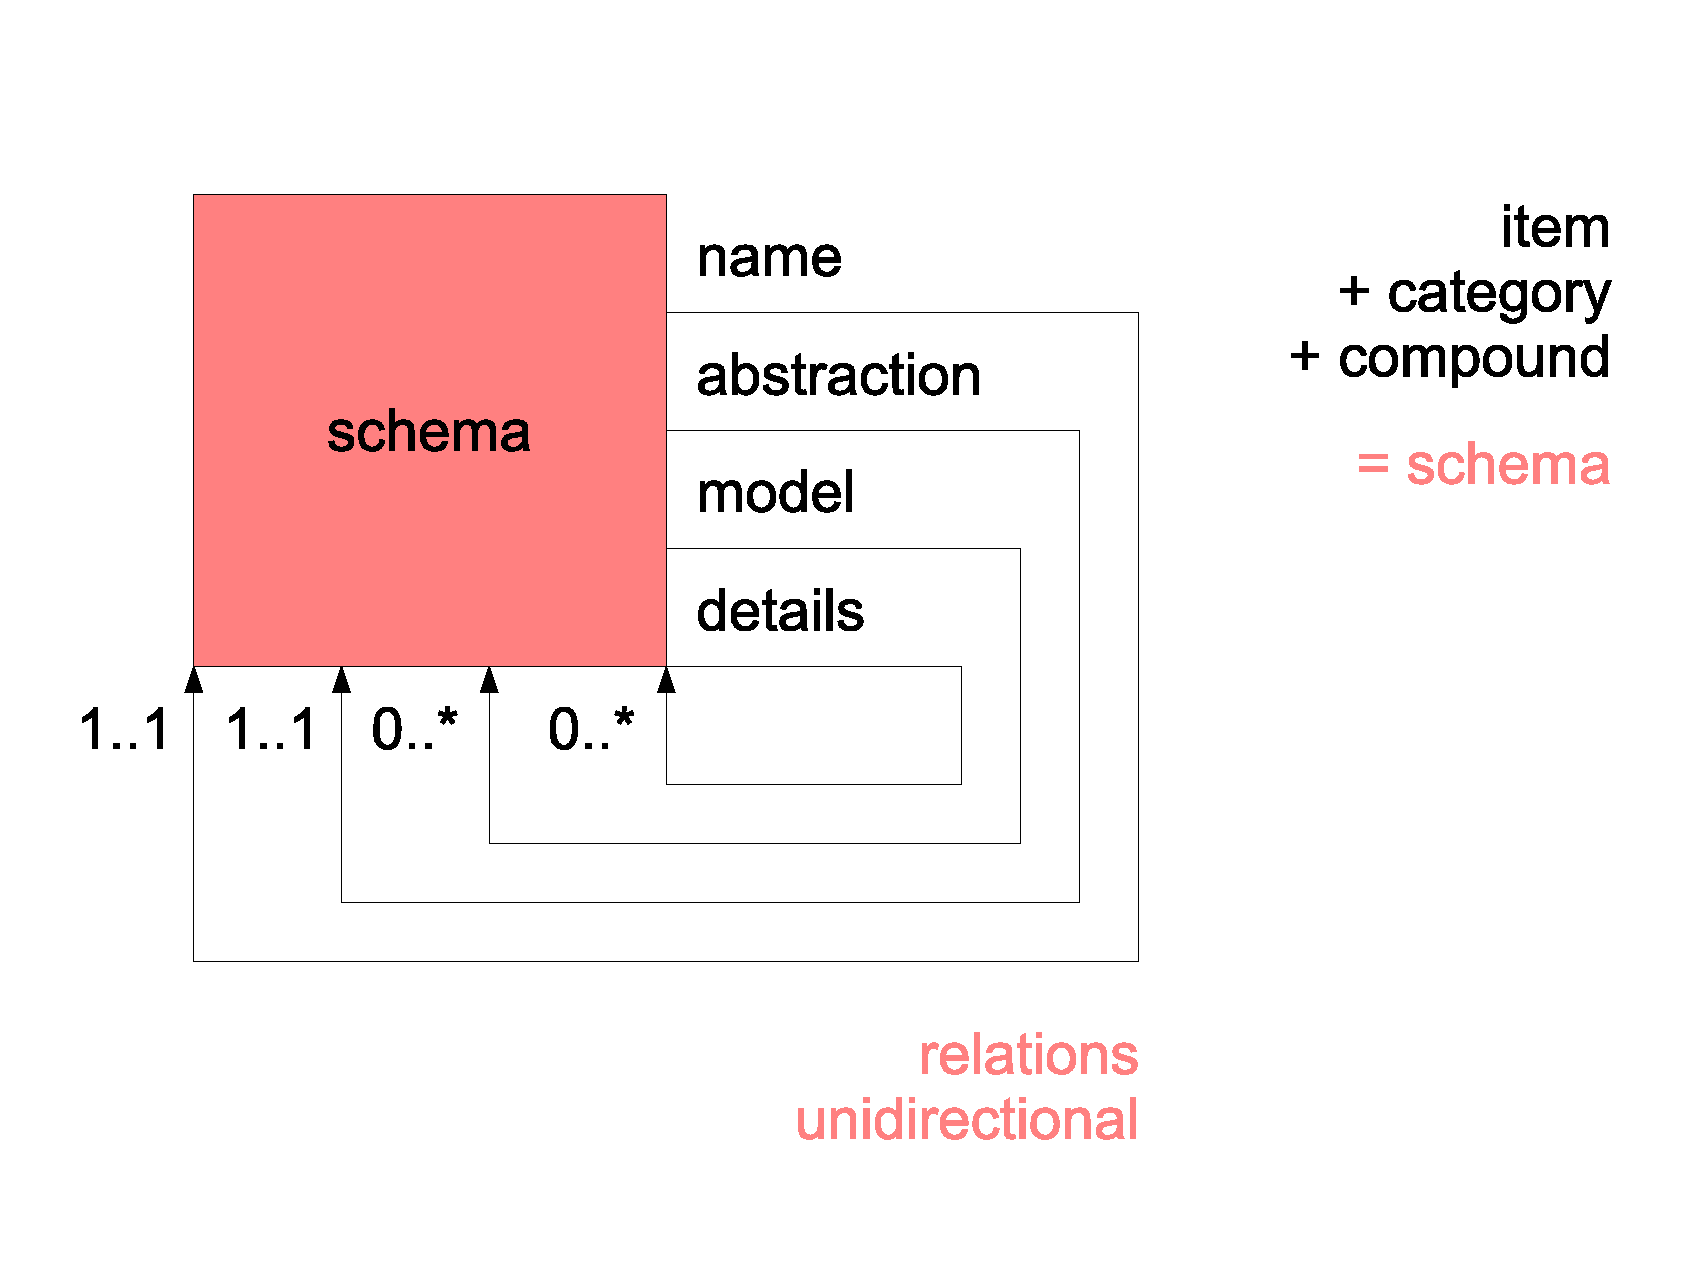
\includegraphics[scale=0.2]{vector/schema.eps}
        \caption{Knowledge Schema}
        \label{schema_figure}
    \end{center}
\end{figure}

Yet what does this knowledge of a compound model (whole) about its parts imply?
Software developers call knowledge \emph{about} something
\emph{Meta Information}. Figure \ref{schema_figure} illustrates a
\emph{Schema} (structure) with four kinds of meta information in a whole-part
relation.

An obvious way is to give each part a unique \emph{Name} for identification.
Secondly, a compound needs to know about the \emph{Model} of each part since a
part may itself be seen as compound that needs to know about its parts. The
distinction of the several kinds of models, in other words the kind of
\emph{Abstraction} (compound, term, number etc.) of a model is the third kind
of information a compound needs to know about its parts. It is comparable to a
\emph{Type} in classical system programming languages. All further kinds of
meta information are summed up by a fourth relation which is called
\emph{Details}.

%
% $RCSfile: double_hierarchy.tex,v $
%
% Copyright (C) 2002-2008. Christian Heller.
%
% Permission is granted to copy, distribute and/or modify this document
% under the terms of the GNU Free Documentation License, Version 1.1 or
% any later version published by the Free Software Foundation; with no
% Invariant Sections, with no Front-Cover Texts and with no Back-Cover
% Texts. A copy of the license is included in the section entitled
% "GNU Free Documentation License".
%
% http://www.cybop.net
% - Cybernetics Oriented Programming -
%
% http://www.resmedicinae.org
% - Information in Medicine -
%
% Version: $Revision: 1.1 $ $Date: 2008-08-19 20:41:06 $ $Author: christian $
% Authors: Christian Heller <christian.heller@tuxtax.de>
%

\subsection{Double Hierarchy}
\label{double_hierarchy_heading}
\index{Double Hierarchy}
\index{Whole-Part Relationship}
\index{Dialectical Relationship between Whole and Part}
\index{Conceptual Interaction}
\index{Part}
\index{Property}
\index{Constraint}

Finally, what makes up the character of a model (in the understanding of the
human mind) is a combination of two hierarchies: the \emph{Parts} it consists
of, together with \emph{Meta Information} about it.

Most properties of a molecule in \emph{Chemistry}, for example, are determined
by the number and arrangement of its atoms. \emph{Hydrogen} (H$_{2}$) becomes
\emph{Water} (H$_{2}$O) (with a totally different character) when just one
\emph{Oxygen} (O) atom is added per hydrogen molecule. The Wikipedia Encyclopedia
\cite{wikipedia} cites and writes about Richard Levins and Richard Lewontin
who, in their book \textit{The Dialectical Biologist} \cite{levins}, sketch a
\emph{dialectical} approach to biology:

\begin{quote}
    They focus on the (dialectical) relationship between the \emph{Whole} (or
    \emph{Totality}) and the \emph{Parts}: \textit{Part makes Whole, and Whole
    makes Part} \cite[p. 272]{levins}. That is, a biological system of some kind
    consists of a collection of heterogeneous parts. All of these contribute to
    the character of the whole, as in reductionist thinking. On the other hand,
    the whole has an existence independent of the parts and feeds back to affect
    and determine the nature of the parts. This back-and-forth (dialectic) of
    causation implies a dynamic process. \ldots\ Further, each species is part
    of the \emph{Environment} of all of the others.
\end{quote}

The kinds of meta information discussed in the previous sections were also
called \emph{Dimensions} or \emph{Conceptual Interaction} between a \emph{Whole}
and its \emph{Parts}. They may represent very different properties and each of
them may be constrained to certain values- or areas of validity.

\begin{figure}[ht]
    \begin{center}
        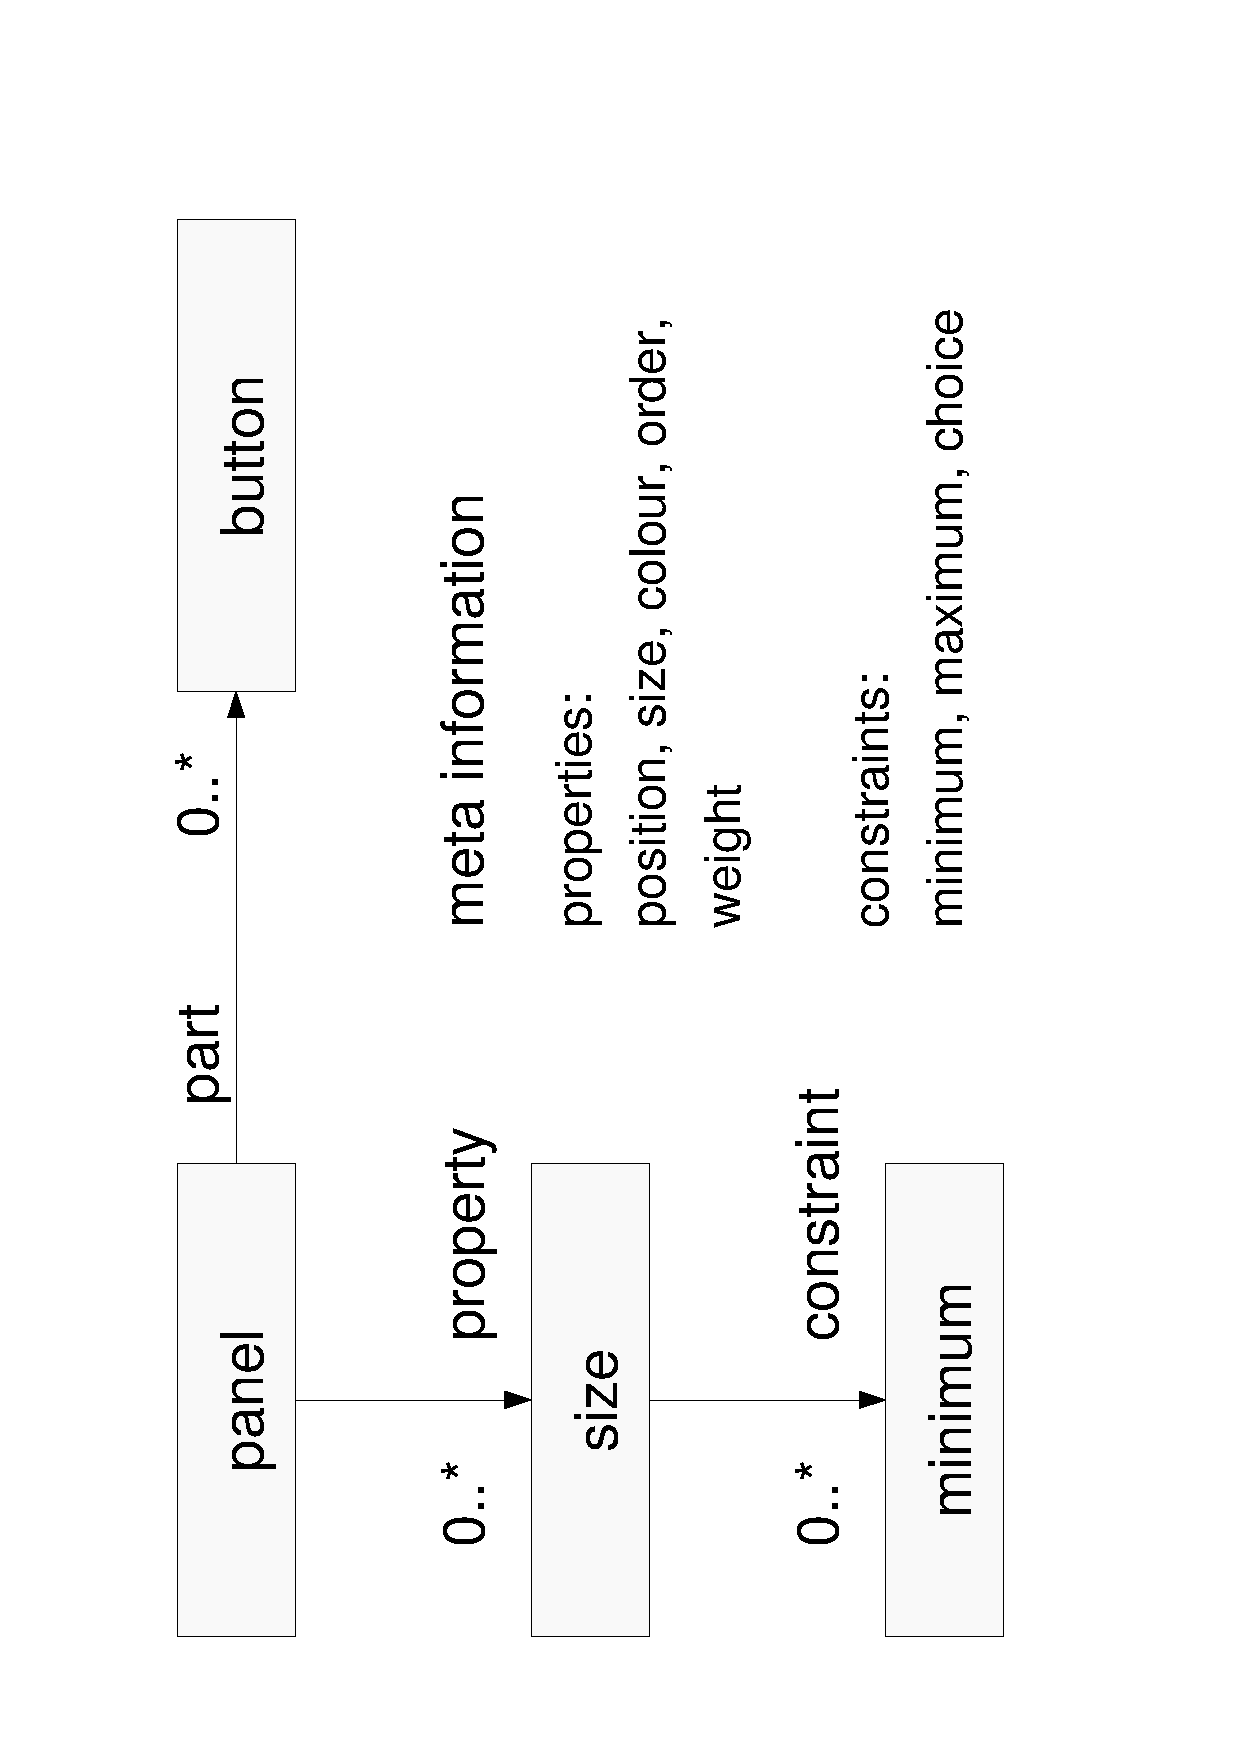
\includegraphics[scale=0.3,angle=-90]{graphic/double.pdf}
        \caption{Double Hierarchy of Parts and Meta Information}
        \label{double_figure}
    \end{center}
\end{figure}

Figure \ref{double_figure} illustrates the \emph{Double Hierarchy} here
spoken of. A graphical panel was chosen as example model. It may consist of
smaller parts, among them being a number of buttons. Altogether, they form the
\emph{Part Hierarchy}. On the other hand, there are properties like the size,
position or colour of the buttons, which are neither part of the panel, nor of
the buttons themselves; they are information \emph{about} the buttons and form
an own \emph{Meta Hierarchy}. To the latter do also belong constraints like the
minimum size of a button or a possible choice of colours for it. Constraints can
be treated like meta information about properties. Once again: \emph{Properties}
are information about a \emph{Part}; \emph{Constraints} are information about a
\emph{Property}.


\newpage{\pagestyle{empty}\cleardoublepage}
%
% $RCSfile: state_and_logic.tex,v $
%
% Copyright (c) 2005-2006. Christian Heller. All rights reserved.
%
% Permission is granted to copy, distribute and/or modify this document
% under the terms of the GNU Free Documentation License, Version 1.1 or
% any later version published by the Free Software Foundation; with no
% Invariant Sections, with no Front-Cover Texts and with no Back-Cover
% Texts. A copy of the license is included in the section entitled
% "GNU Free Documentation License".
%
% http://www.cybop.net
% - Cybernetics Oriented Programming -
%
% http://www.resmedicinae.org
% - Information in Medicine -
%
% Version: $Revision: 1.1 $ $Date: 2006-01-03 08:21:45 $ $Author: christian $
% Authors: Christian Heller <christian.heller@tuxtax.de>
%

\subsection{State and Logic}
\label{state_and_logic_heading}

According to the observations made in the work described in this article, there
are two kinds of knowledge: \emph{State-} and \emph{Logic}. While the former
may be placed in a spatial dimension, the latter is processed as sequence over
time. Often, logic is labelled \emph{dynamic} behaviour -- but only the
\emph{execution} of a rule of logic is dynamic, \emph{not} the rule itself
(\emph{static}).

Rules of logic translate input- into output states. What
characterises a system is how it applies logic knowledge to translate state
knowledge \cite{heller2002}. Yet how to imagine a knowledge model consisting of
state- as well as logic parts? Following an example.

The famous \emph{Model View Controller} (MVC) pattern was extended by the
\emph{Hierarchical MVC} (HMVC) pattern towards a hierarchy of \emph{MVC Triads}
\cite{cai}. The omnipresence of hierarchies in the MVC was demonstrated in
\cite{hellerbohl}.

\begin{figure}[ht]
    \begin{center}
        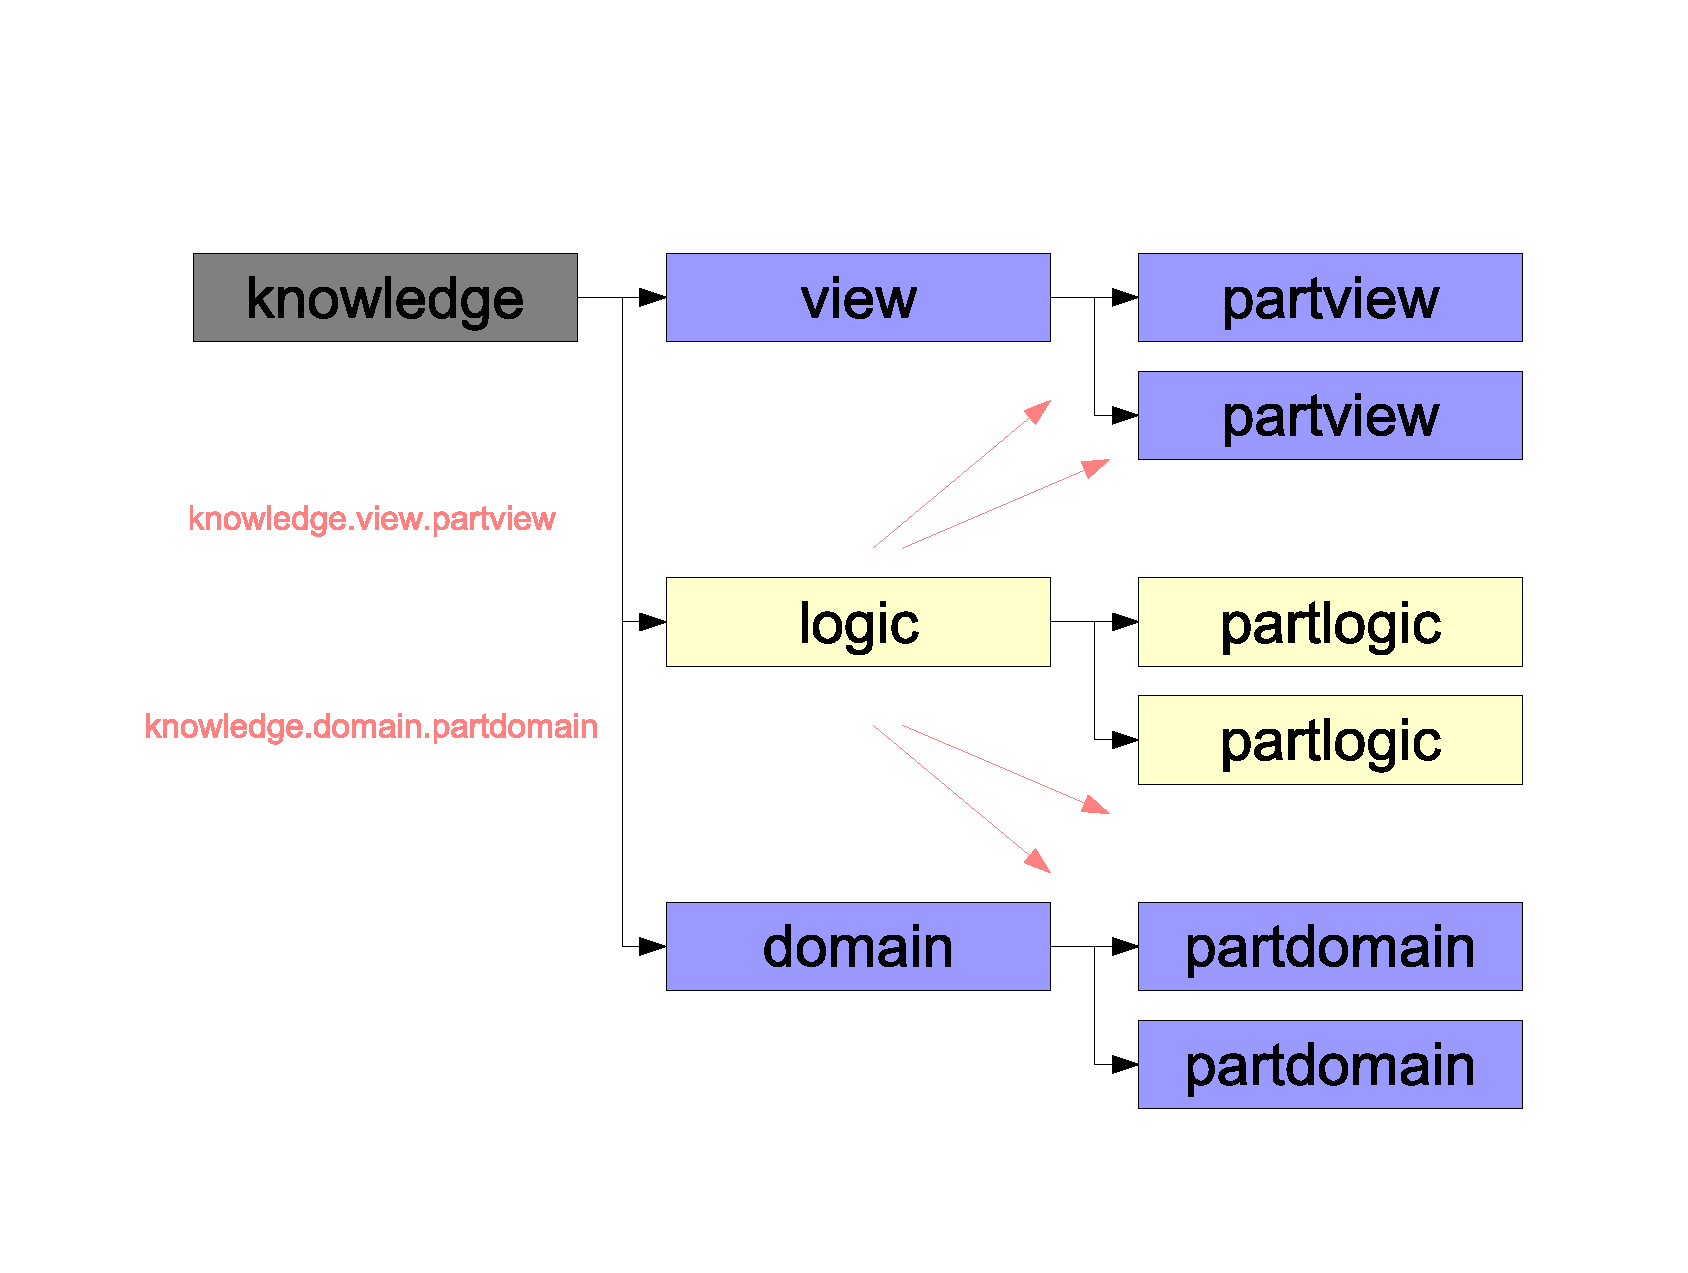
\includegraphics[scale=0.2]{vector/mvctree.eps}
        \caption{Runtime Logic manipulating States}
        \label{mvctree_figure}
    \end{center}
\end{figure}

Figure \ref{mvctree_figure} shows the three parts: \emph{Domain} (Model),
\emph{View} and \emph{Logic} (Controller) of an (adapted) MVC pattern as
independent branches of one common knowledge tree, as existent at system
runtime in memory. Each of them represents a concept on its own. The logic
model, however, is allowed to access and change the view- and domain model; it
is able to link different knowledge models. But view- and domain model,
representing states, are not allowed to manipulate logic. In other words: The
dependencies between logic- and state models are \emph{unidirectional}.

An innovation is that logic knowledge gets manipulatable. A logic model
(algorithm) cannot only access and change state-, but also logic models, even
itself! Because models modified in that manner can be made persistent in form
of CYBOL knowledge templates (section \ref{practical_proof_heading}), and be
reloaded the next time an application starts, this may be seen as a kind of
\emph{Meta Programming} \cite{wikipedia}.

The clear separation of states and logic into discrete models avoids unwanted
dependencies as caused by the bundling of attributes and methods in OOP. All
that would be needed to make a CYBOP system work with new state models, is the
corresponding translation logic. Translators \cite{hellerkunze} simplify
architectures and unify communication.


    \newpage{\pagestyle{empty}\cleardoublepage}
    %
% $RCSfile: proof.tex,v $
%
% Copyright (C) 2002-2008. Christian Heller.
%
% Permission is granted to copy, distribute and/or modify this document
% under the terms of the GNU Free Documentation License, Version 1.1 or
% any later version published by the Free Software Foundation; with no
% Invariant Sections, with no Front-Cover Texts and with no Back-Cover
% Texts. A copy of the license is included in the section entitled
% "GNU Free Documentation License".
%
% http://www.cybop.net
% - Cybernetics Oriented Programming -
%
% http://www.resmedicinae.org
% - Information in Medicine -
%
% Version: $Revision: 1.1 $ $Date: 2008-08-19 20:41:08 $ $Author: christian $
% Authors: Christian Heller <christian.heller@tuxtax.de>
%

\part{Proof}
\label{proof_heading}
\newpage{\pagestyle{empty}\cleardoublepage}

%
% $RCSfile: cybernetics_oriented_language.tex,v $
%
% Copyright (c) 2001-2004. Christian Heller. All rights reserved.
%
% No copying, altering, distribution or any other actions concerning this
% document, except after explicit permission by the author!
% At some later point in time, this document is planned to be put under
% the GNU FDL license. For now, _everything_ is _restricted_ by the author.
%
% http://www.cybop.net
% - Cybernetics Oriented Programming -
%
% http://www.resmedicinae.org
% - Information in Medicine -
%
% @author Christian Heller <christian.heller@tuxtax.de>
%

\section{Cybernetics Oriented Language}
\label{cybernetics_oriented_language_heading}

The introduced \emph{Cybernetics Oriented Language} (CYBOL) is based on the
principles of \emph{Human Thinking} as described in section \ref{human_thinking_heading}.
These principles and further concepts behind are summarized by the name
\emph{Cybernetics Oriented Programming} (CYBOP) (figure \ref{cybop_figure}).
They form the semantics of CYBOL. Its syntax is determined by the \emph{Extensible
Markup Language} (XML) standard and accordingly easy. It is rich enough to express
models based upon the three kinds of abstraction: \emph{Discrimination},
\emph{Categorization} and \emph{Composition} as well as meta information of a
\emph{Whole} about its \emph{Parts}.

\begin{figure}[ht]
    \begin{center}
        
\includegraphics[scale=0.3]{vector/cybop.eps}
        \caption{CYBOP}
        \label{cybop_figure}
    \end{center}
\end{figure}

%
% $RCSfile: syntax.tex,v $
%
% Copyright (C) 2002-2008. Christian Heller.
%
% Permission is granted to copy, distribute and/or modify this document
% under the terms of the GNU Free Documentation License, Version 1.1 or
% any later version published by the Free Software Foundation; with no
% Invariant Sections, with no Front-Cover Texts and with no Back-Cover
% Texts. A copy of the license is included in the section entitled
% "GNU Free Documentation License".
%
% http://www.cybop.net
% - Cybernetics Oriented Programming -
%
% http://www.resmedicinae.org
% - Information in Medicine -
%
% Version: $Revision: 1.1 $ $Date: 2008-08-19 20:41:09 $ $Author: christian $
% Authors: Christian Heller <christian.heller@tuxtax.de>
%

\subsection{Syntax}
\label{syntax_heading}
\index{CYBOL Syntax}
\index{Syntax of a Language}
\index{Grammar of a Language}
\index{Extensible Markup Language}
\index{XML}
\index{XML Tag}
\index{XML Attribute}
\index{Discrimination}
\index{Composition}

Every language has a special \emph{Syntax}, that is a \emph{Grammar} with rules
for combining terms and symbols \cite{foldoc}. CYBOL could define its own
syntax or use an already existing one, of another language. Because of its
popularity, clear text representation, flexibility, extensibility and ease of
use, \emph{XML} was chosen to deliver the syntax for CYBOL.

To mention just two of the syntactical elements of XML, \emph{Tag} and
\emph{Attribute} are considered shortly here. Tags are special, arbitrary
keywords that have to be defined by the system working with an XML document.
Attributes keep additional information about the contents enclosed by two tags.
Two examples:

\begin{scriptsize}
    \begin{verbatim}
    <tag attribute="value">
        contents
    </tag>
    \end{verbatim}
\end{scriptsize}

\begin{scriptsize}
    \begin{verbatim}
    <tag attribute1="value" attribute2="contents"/>
    \end{verbatim}
\end{scriptsize}

An XML document carries a name and can such represent a \emph{Discrete Item},
as suggested by the principles of human thinking (section
\ref{human_thinking_heading}). Being a \emph{Compound}, it consists of parts --
and, it can link to other documents treated as its parts. That way, a whole
hierarchy can be formed. Tag attributes can keep additional information about
the linked parts. Most importantly, XML documents have a hierarchical structure
based on tags, which may be used to store meta information about a part.

Considering these properties of XML, it seems predestinated for formally
representing abstract models using the CYBOP concepts. CYBOL, finally, is XML
\emph{plus} a defined set of tags, attributes and values, used to structure and
link documents meaningfully.

%
% $RCSfile: vocabulary.tex,v $
%
% Copyright (C) 2002-2008. Christian Heller.
%
% Permission is granted to copy, distribute and/or modify this document
% under the terms of the GNU Free Documentation License, Version 1.1 or
% any later version published by the Free Software Foundation; with no
% Invariant Sections, with no Front-Cover Texts and with no Back-Cover
% Texts. A copy of the license is included in the section entitled
% "GNU Free Documentation License".
%
% http://www.cybop.net
% - Cybernetics Oriented Programming -
%
% http://www.resmedicinae.org
% - Information in Medicine -
%
% Version: $Revision: 1.1 $ $Date: 2008-08-19 20:41:09 $ $Author: christian $
% Authors: Christian Heller <christian.heller@tuxtax.de>
%

\subsection{Vocabulary}
\label{vocabulary_heading}
\index{CYBOL Vocabulary}
\index{Terms of a Language}
\index{Symbols of a Language}
\index{Syntax of a Language}
\index{Document Type Definition}
\index{DTD}
\index{XML Schema Definition}
\index{XSD}
\index{Extended Backus Naur Form}
\index{EBNF}

The \emph{Vocabulary} is what fills a language with life. It delivers the
\emph{Terms} and \emph{Symbols} that are combined after the rules of a syntax.

XML allows to define and exchange the whole vocabulary of a language. It offers
two ways in which a list of legal elements can be defined: The traditional
\emph{Document Type Definition} (DTD) and the more modern
\emph{XML Schema Definition} (XSD). Besides the vocabulary, DTD and XSD define
the structure of an XML document and allow to typify, constrain and validate
items. In addition to DTD and XSD, the \emph{Extended Backus Naur Form} (EBNF)
of CYBOL is given following.

The language definitions were not added as appendix to this work, because
firstly, they are not too long and secondly, an understanding of the CYBOL
elements is necessary to be able to grasp the constructs and examples given in
later sections.

\input{document_type_definition}
\clearpage
\input{xml_schema_definition}
\input{extended_backus_naur_form}
\clearpage

%\input{self_definition}
%Model and Metamodel \cite{sowa}, p. 431 and (for UML): p.436
%- UML needs a meta model describing its graphical model elements
%(Class, Association etc. are treated as classes themselves)
%- XML needs special definition languages (DTD, XSD)
%--> Show that CYBOL is its own meta model and can describe itself!

%
% $RCSfile: semantics.tex,v $
%
% Copyright (C) 2002-2008. Christian Heller.
%
% Permission is granted to copy, distribute and/or modify this document
% under the terms of the GNU Free Documentation License, Version 1.1 or
% any later version published by the Free Software Foundation; with no
% Invariant Sections, with no Front-Cover Texts and with no Back-Cover
% Texts. A copy of the license is included in the section entitled
% "GNU Free Documentation License".
%
% http://www.cybop.net
% - Cybernetics Oriented Programming -
%
% http://www.resmedicinae.org
% - Information in Medicine -
%
% Version: $Revision: 1.1 $ $Date: 2008-08-19 20:41:08 $ $Author: christian $
% Authors: Christian Heller <christian.heller@tuxtax.de>
%

\subsection{Semantics}
\label{semantics_heading}
\index{Semantics of a Language}
\index{CYBOL Semantics}
\index{State Knowledge Modelling}
\index{Logic Knowledge Modelling}
\index{Extensible Markup Language}
\index{XML}
\index{XML Tag}
\index{XML Attribute}

The meaning expressed by terms and sentences is their \emph{Semantics}
\cite{duden}.

CYBOL files can be used to model either \emph{State-} or \emph{Logic Knowledge}
(chapter \ref{state_and_logic_heading}). In both cases, the \emph{same} syntax
(document structure) with \emph{identical} vocabulary (XML tags and -attributes)
is applied. It is the attribute \emph{Values} that make a difference in meaning.

The double hierarchy proposed by CYBOP's knowledge schema (section
\ref{knowledge_representation_heading}) is put into static CYBOL knowledge
templates, by using XML \emph{Attributes} for representing the whole-part
hierarchy, and XML \emph{Tags} for representing the additional meta information
that a whole model keeps about its part models.

\input{attributes}
\input{tags}

%
% $RCSfile: example.tex,v $
%
% Copyright (c) 2001-2004. Christian Heller. All rights reserved.
%
% No copying, altering, distribution or any other actions concerning this
% document, except after explicit permission by the author!
% At some later point in time, this document is planned to be put under
% the GNU FDL license. For now, _everything_ is _restricted_ by the author.
%
% http://www.cybop.net
% - Cybernetics Oriented Programming -
%
% http://www.resmedicinae.org
% - Information in Medicine -
%
% @author Christian Heller <christian.heller@tuxtax.de>
%

\subsection{Example}
\label{example_heading}

The following example shows a minimalistic model of a (static) \emph{Graphical
User Interface} (GUI) frame.

\begin{verbatim}
<!--
    frame_example.cybol
/-->
<model>
    <part name="title"
        part_abstraction="string"
        part_model="Res Medicinae"/>
    <part name="menu_bar"
        part_abstraction="compound"
        part_model="/gui/menu_bar.cybol"
        position_abstraction="compass"
        position_model="north"/>
    <part name="status_bar"
        part_abstraction="compound"
        part_model="/gui/tool_bar.cybol"
        position_abstraction="compass"
        position_model="south"/>
</model>
\end{verbatim}

Similar models can be built of (dynamic) workflows whereby the inputs and outputs
of the part operations appear in a special order as attribute values. But this
may become the topic of a follow-up paper.


\newpage{\pagestyle{empty}\cleardoublepage}
%
% $RCSfile: cybernetics_oriented_interpreter.tex,v $
%
% Copyright (C) 2002-2008. Christian Heller.
%
% Permission is granted to copy, distribute and/or modify this document
% under the terms of the GNU Free Documentation License, Version 1.1 or
% any later version published by the Free Software Foundation; with no
% Invariant Sections, with no Front-Cover Texts and with no Back-Cover
% Texts. A copy of the license is included in the section entitled
% "GNU Free Documentation License".
%
% http://www.cybop.net
% - Cybernetics Oriented Programming -
%
% http://www.resmedicinae.org
% - Information in Medicine -
%
% Version: $Revision: 1.1 $ $Date: 2008-08-19 20:41:06 $ $Author: christian $
% Authors: Christian Heller <christian.heller@tuxtax.de>
%

\chapter{Cybernetics Oriented Interpreter}
\label{cybernetics_oriented_interpreter_heading}
\index{Cybernetics Oriented Interpreter}
\index{CYBOI}

\begin{flushright}
    \textsl{
        Two Things are needed to do our Work:\\
        tireless Endurance and the Willingness to throw something,\\
        that has cost much Time and Effort, away again.
    }\\
    \textsc{Albert Einstein}
\end{flushright}

The previous chapter described how the CYBOP concepts introduced in part
\ref{contribution_heading} of this work can be implemented in a formal language
carrying the abbreviated name CYBOL. The now still missing piece is a program
able to dynamically handle static CYBOL sources, as mentioned in chapter
\ref{statics_and_dynamics_heading}. This chapter therefore describes the
\emph{Cybernetics Oriented Interpreter} (CYBOI) \cite{cybop} which can do just
that.

%
% $RCSfile$
%
% Copyright (c) 2005-2006. Christian Heller. All rights reserved.
%
% Permission is granted to copy, distribute and/or modify this document
% under the terms of the GNU Free Documentation License, Version 1.1 or
% any later version published by the Free Software Foundation; with no
% Invariant Sections, with no Front-Cover Texts and with no Back-Cover
% Texts. A copy of the license is included in the section entitled
% "GNU Free Documentation License".
%
% http://www.cybop.net
% - Cybernetics Oriented Programming -
%
% http://www.resmedicinae.org
% - Information in Medicine -
%
% Version: $Revision$ $Date$ $Author$
% Authors: Christian Heller <christian.heller@tuxtax.de>
%

\subsubsection{Architecture}
\label{architecture_heading}

To what concerns its inner architecture, there are two basic structures
underlying CYBOI:

\begin{enumerate}
    \item \emph{Knowledge Container:} An array-based structure usable for
        storing static knowledge in form of primitive- and compound models, and
        capable of representing a map, collection, list and tree
    \item \emph{Signal Checker:} A loop-based structure usable for dynamically
        reading signals from a queue, and capable of processing them after
        their priority, in a special handler
\end{enumerate}

\begin{figure}[ht]
    \begin{center}
        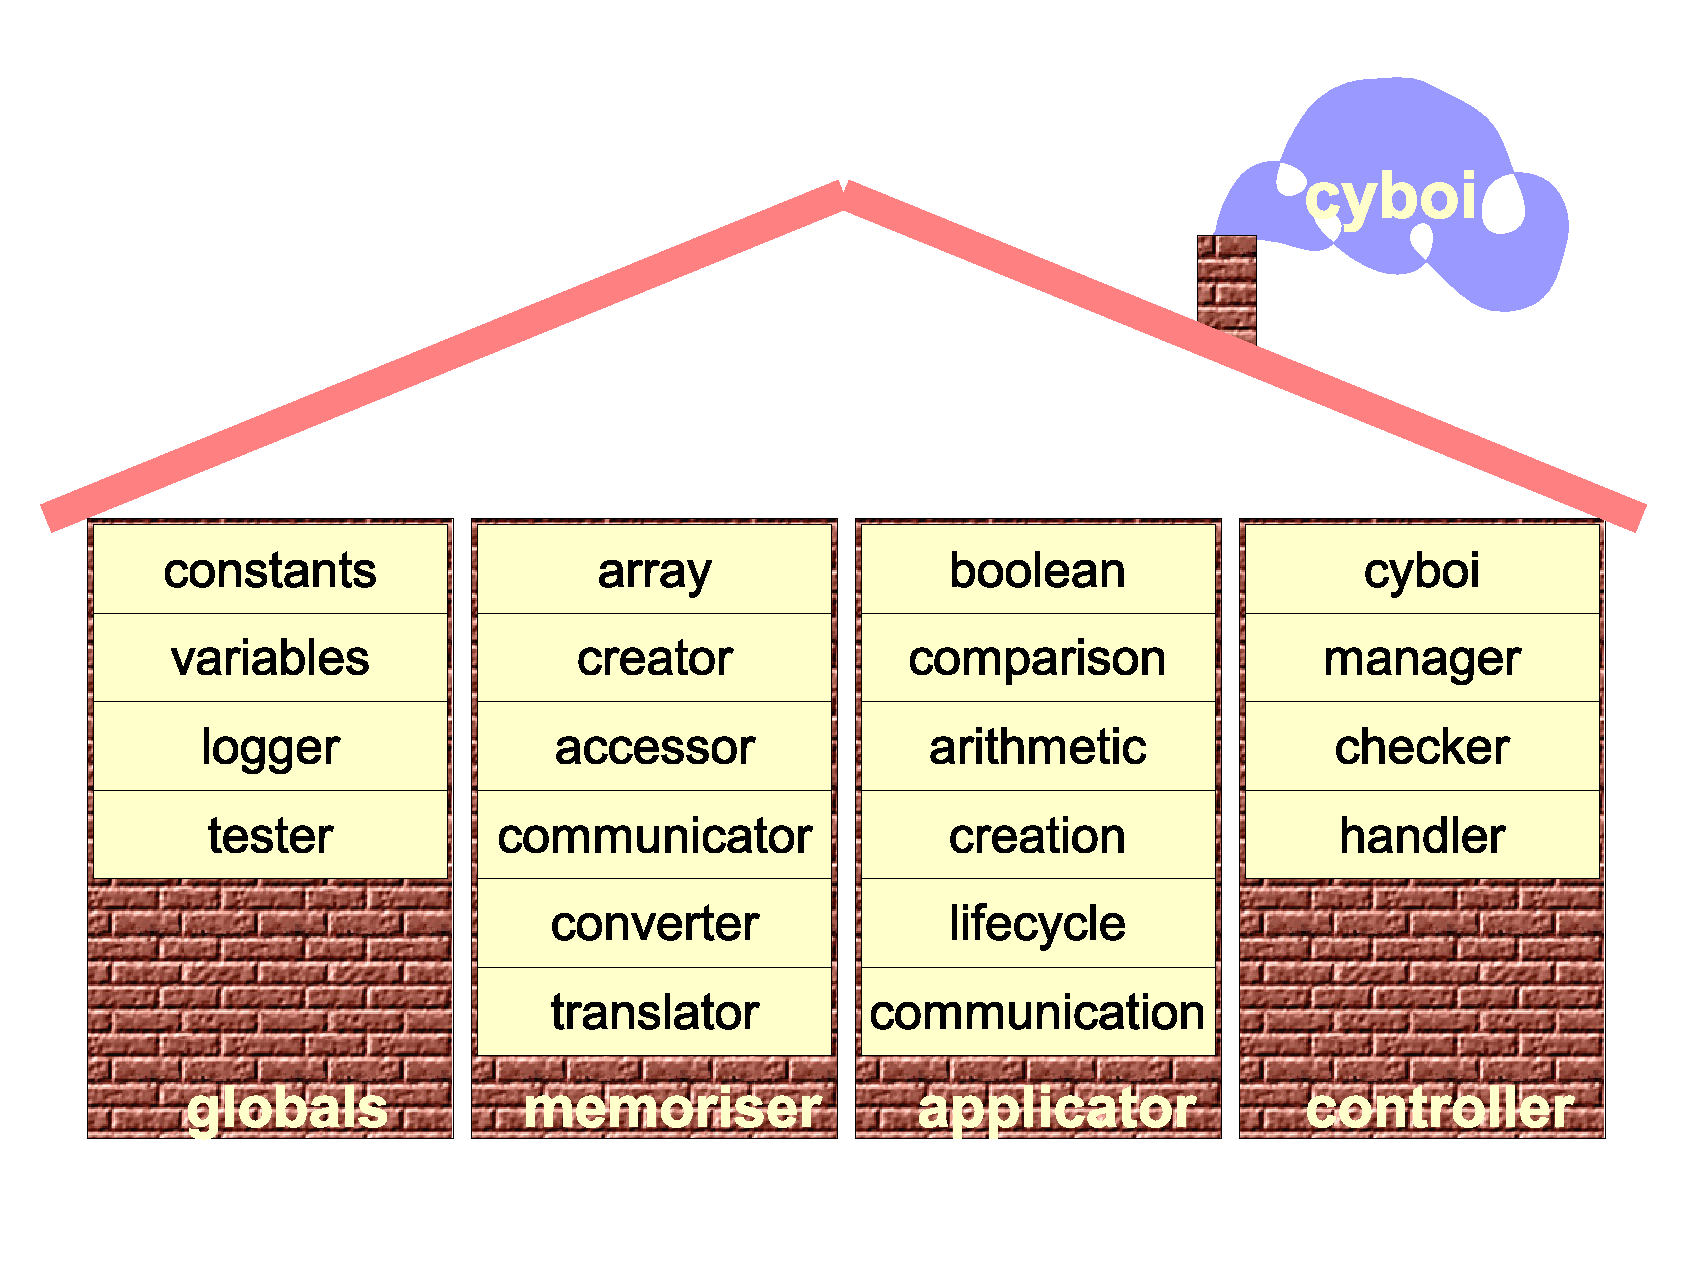
\includegraphics[scale=0.2]{vector/architecture.eps}
        \caption{CYBOI Architecture}
        \label{architecture_figure}
    \end{center}
\end{figure}

All modules, into which CYBOI is subdivided, are built around these two core
structures. Not unlike John von Neumann's model of a computing machine
\cite{selflinux}, which distinguishes \emph{Memory}, \emph{Control Unit},
\emph{Algorithmic Logic Unit} (ALU) and \emph{Input/ Output} (i/o), CYBOI's
modules are grouped into four architectural parts, as illustrated in figure
\ref{architecture_figure}. These have the following functionality:

\begin{itemize}
    \item \emph{Memoriser:} data creation, -destruction and -access (after
        Neumann, it contains not only data, but also the operations that are
        applied to them)
    \item \emph{Controller:} lifecycle management, signal handling, i/o filters
    \item \emph{Applicator:} operation application (comparison, logic,
        arithmetic and more)
    \item \emph{Globals:} basic constants and variables, as well as a logger
\end{itemize}

The i/o data handling is not separated out here (as opposed to von Neumann's
model); it is managed by the controller modules. The i/o data themselves,
representing states, are stored in memory.

%
% $RCSfile: functionality_in_detail.tex,v $
%
% Copyright (C) 2002-2008. Christian Heller.
%
% Permission is granted to copy, distribute and/or modify this document
% under the terms of the GNU Free Documentation License, Version 1.1 or
% any later version published by the Free Software Foundation; with no
% Invariant Sections, with no Front-Cover Texts and with no Back-Cover
% Texts. A copy of the license is included in the section entitled
% "GNU Free Documentation License".
%
% http://www.cybop.net
% - Cybernetics Oriented Programming -
%
% http://www.resmedicinae.org
% - Information in Medicine -
%
% Version: $Revision: 1.1 $ $Date: 2008-08-19 20:41:06 $ $Author: christian $
% Authors: Christian Heller <christian.heller@tuxtax.de>
%

\section{Functionality in Detail}
\label{functionality_in_detail_heading}
\index{CYBOI Functionality}
\index{CYBOI Part Dependencies}
\index{CYBOI Control Flow}

CYBOI's architecture is based on three main parts, as introduced by figure
\ref{architecture_figure} before: \emph{Controller}, \emph{Applicator} and
\emph{Memoriser}. (The \emph{Globals} package is neglectable for the following
explanations, since it contains static constants and variables that are
\emph{omnipresent}.) They appear again in figure \ref{dependencies_figure}
which shows the \emph{Dependencies} between them. Additionally, the
\emph{Controller} modules and their \emph{Control Flow} is illustrated.
Starting from the \emph{cyboi} module, the following subsections will
demonstrate how CYBOI functions internally, along the flow of control touching
the modules: \emph{manager}, \emph{checker} and \emph{handler}. After that, the
execution of operations in the \emph{Applicator} as well as the creation and
transition of data in the \emph{Memoriser} are described.

\begin{figure}[ht]
    \begin{center}
        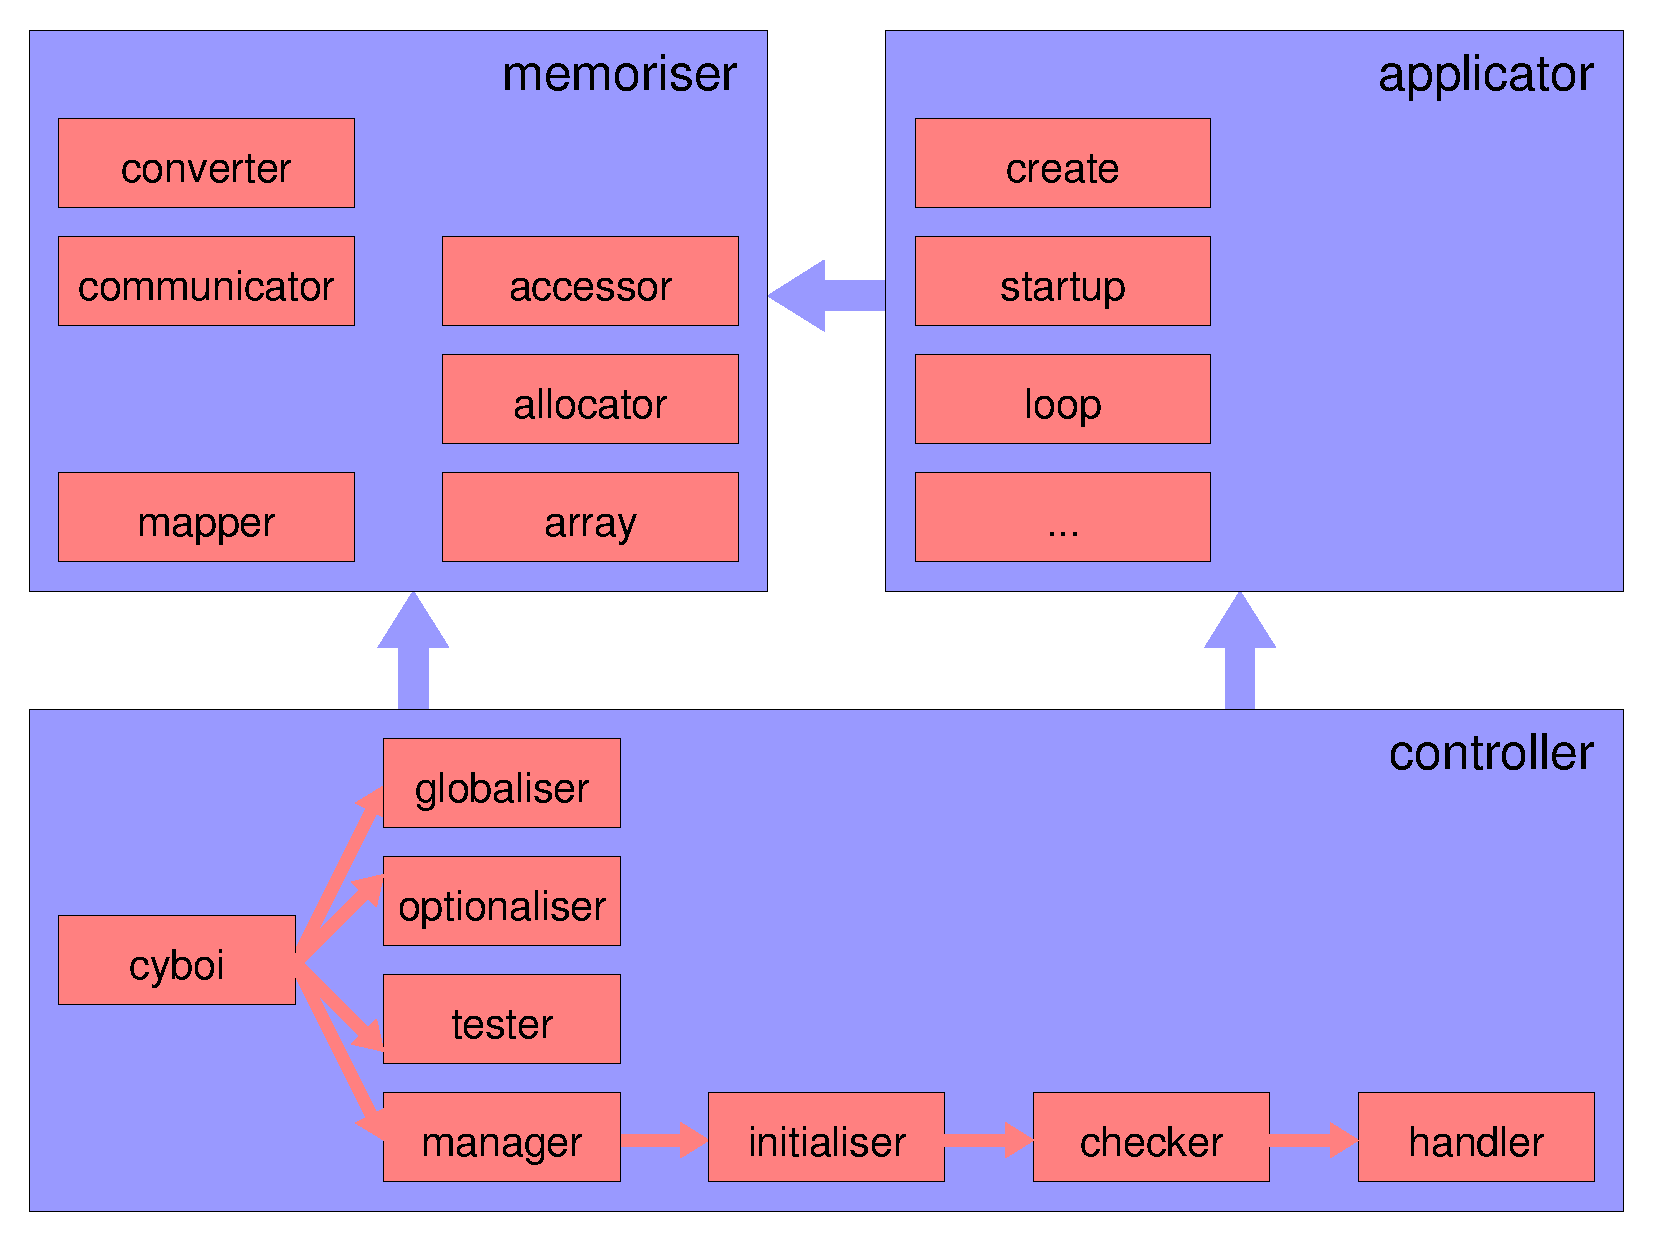
\includegraphics[scale=0.3,angle=-90]{graphic/dependencies.pdf}
        \caption{CYBOI Part Dependencies and Control Flow}
        \label{dependencies_figure}
    \end{center}
\end{figure}

\input{process_launching}
\input{lifecycle_management}
\input{signal_checking}
\input{signal_handling}
\input{operation_execution}
\input{model_transition}
\input{data_creation}
%\input{instance}

%
% $RCSfile: implementation.tex,v $
%
% Copyright (C) 2002-2008. Christian Heller.
%
% Permission is granted to copy, distribute and/or modify this document
% under the terms of the GNU Free Documentation License, Version 1.1 or
% any later version published by the Free Software Foundation; with no
% Invariant Sections, with no Front-Cover Texts and with no Back-Cover
% Texts. A copy of the license is included in the section entitled
% "GNU Free Documentation License".
%
% http://www.cybop.net
% - Cybernetics Oriented Programming -
%
% http://www.resmedicinae.org
% - Information in Medicine -
%
% Version: $Revision: 1.1 $ $Date: 2008-08-19 20:41:07 $ $Author: christian $
% Authors: Christian Heller <christian.heller@tuxtax.de>
%

\section{Implementation}
\label{implementation_heading}
\index{CYBOI Implementation}

This section describes some issues that arose during implementation, and how
they are addressed in CYBOI.

\input{simplified_c}
\input{corrected_c}
\input{used_libraries}
\input{development_environment}
\input{error_handling}
\input{distribution_and_installation}


\newpage{\pagestyle{empty}\cleardoublepage}
%
% $RCSfile: res_medicinae.tex,v $
%
% Copyright (C) 2002-2008. Christian Heller.
%
% Permission is granted to copy, distribute and/or modify this document
% under the terms of the GNU Free Documentation License, Version 1.1 or
% any later version published by the Free Software Foundation; with no
% Invariant Sections, with no Front-Cover Texts and with no Back-Cover
% Texts. A copy of the license is included in the section entitled
% "GNU Free Documentation License".
%
% http://www.cybop.net
% - Cybernetics Oriented Programming -
%
% http://www.resmedicinae.org
% - Information in Medicine -
%
% Version: $Revision: 1.1 $ $Date: 2008-08-19 20:41:08 $ $Author: christian $
% Authors: Christian Heller <christian.heller@tuxtax.de>
%

\chapter{Res Medicinae}
\label{res_medicinae_heading}
\index{Res Medicinae Application Prototype}

\begin{flushright}
    \textsl{
        No Road can ever be too long,\\
        side-by-side with a good Friend.
    }\\
    \textsc{Unknown Author}
\end{flushright}

The first two chapters (\ref{cybernetics_oriented_language_heading} and
\ref{cybernetics_oriented_interpreter_heading}) of part \ref{proof_heading} of
this work defined the CYBOL language and its corresponding interpreter CYBOI.
Since a theory is worth more if it can be proven in practice, this chapter will
describe an effort trying to apply both to create an application system named
\emph{Res Medicinae} \cite{resmedicinae} (Latin for \emph{Matter of Medicine}).

%
% $RCSfile: project.tex,v $
%
% Copyright (C) 2002-2008. Christian Heller.
%
% Permission is granted to copy, distribute and/or modify this document
% under the terms of the GNU Free Documentation License, Version 1.1 or
% any later version published by the Free Software Foundation; with no
% Invariant Sections, with no Front-Cover Texts and with no Back-Cover
% Texts. A copy of the license is included in the section entitled
% "GNU Free Documentation License".
%
% http://www.cybop.net
% - Cybernetics Oriented Programming -
%
% http://www.resmedicinae.org
% - Information in Medicine -
%
% Version: $Revision: 1.1 $ $Date: 2008-08-19 20:41:08 $ $Author: christian $
% Authors: Christian Heller <christian.heller@tuxtax.de>
%

\section{Project}
\label{project_heading}
\index{Res Medicinae Project}
\index{Hospital Information System}
\index{HIS}
\index{Practice Management System}
\index{PMS}
\index{Electronic Health Record}
\index{EHR}

The -- somewhat idealistic -- aim was initially to create the prototype of a
\emph{Hospital Information System} (HIS). Due to the clearly too high-set aims,
this was later revised so that the focus of the prototype became a standard
\emph{Practice Management System} (PMS) with an \emph{Electronic Health Record}
(EHR) as its core. Several technology changes during the progress of this work
and the lack in time required to also revise this aim, so that now the final
prototype consists of just the (rudimentary) address management module of the
planned EHR application. It is written in CYBOL and executable by CYBOI.

The following sections describe the project background of \emph{Res Medicinae}.

\input{free_and_open_source_software}
\input{portals_and_services}
\input{tools}
\input{contributors}

%
% $RCSfile: analysis.tex,v $
%
% Copyright (C) 2002-2008. Christian Heller.
%
% Permission is granted to copy, distribute and/or modify this document
% under the terms of the GNU Free Documentation License, Version 1.1 or
% any later version published by the Free Software Foundation; with no
% Invariant Sections, with no Front-Cover Texts and with no Back-Cover
% Texts. A copy of the license is included in the section entitled
% "GNU Free Documentation License".
%
% http://www.cybop.net
% - Cybernetics Oriented Programming -
%
% http://www.resmedicinae.org
% - Information in Medicine -
%
% Version: $Revision: 1.1 $ $Date: 2008-08-19 20:41:05 $ $Author: christian $
% Authors: Christian Heller <christian.heller@tuxtax.de>
%

\section{Analysis}
\label{analysis_heading}
\index{Res Medicinae Requirements Analysis}
\index{Software Engineering Process}
\index{SEP}
\index{Electronic Health Record}
\index{EHR}

Abiding by the standard \emph{Software Engineering Process} (SEP) (chapter
\ref{software_engineering_process_heading}), a \emph{Requirements Analysis}
stood as first activity for the development of \emph{Res Medicinae}. The
following sections will give a brief overview of some requirements and current
modelling trends, concerning the \emph{Electronic Health Record} (EHR). They do
\emph{not} try to replace more comprehensive works written on the subject.

\input{requirements_document}
\input{ehr_and_co}
\input{episode_based}
\input{evidence_based}
\input{continuity_of_care}
\input{core_model}

\newpage
%
% $RCSfile: standards.tex,v $
%
% Copyright (C) 2002-2008. Christian Heller.
%
% Permission is granted to copy, distribute and/or modify this document
% under the terms of the GNU Free Documentation License, Version 1.1 or
% any later version published by the Free Software Foundation; with no
% Invariant Sections, with no Front-Cover Texts and with no Back-Cover
% Texts. A copy of the license is included in the section entitled
% "GNU Free Documentation License".
%
% http://www.cybop.net
% - Cybernetics Oriented Programming -
%
% http://www.resmedicinae.org
% - Information in Medicine -
%
% Version: $Revision: 1.1 $ $Date: 2008-08-19 20:41:09 $ $Author: christian $
% Authors: Christian Heller <christian.heller@tuxtax.de>
%

\section{Standards}
\label{standards_heading}
\index{Medical Informatics Standards}

In a further thought, current standards of medical informatics had to be
considered for the development of \emph{Res Medicinae} application modules.
There exists a whole plethora of (partly \emph{de facto}) standards -- far too
many to discuss here. The following sections will give a brief overview of only
a few standards which are potentially important for EHR development.

\input{overview}
\input{record_modelling}
\input{messaging_and_communication}
\input{terminology_systems}
\input{further_standards}
\input{standards_development}
\input{implication}

%
% $RCSfile: realisation.tex,v $
%
% Copyright (C) 2002-2008. Christian Heller.
%
% Permission is granted to copy, distribute and/or modify this document
% under the terms of the GNU Free Documentation License, Version 1.1 or
% any later version published by the Free Software Foundation; with no
% Invariant Sections, with no Front-Cover Texts and with no Back-Cover
% Texts. A copy of the license is included in the section entitled
% "GNU Free Documentation License".
%
% http://www.cybop.net
% - Cybernetics Oriented Programming -
%
% http://www.resmedicinae.org
% - Information in Medicine -
%
% Version: $Revision: 1.1 $ $Date: 2008-08-19 20:41:08 $ $Author: christian $
% Authors: Christian Heller <christian.heller@tuxtax.de>
%

\section{Realisation}
\label{realisation_heading}
\index{Res Medicinae Steps of Realisation}

Having analysed the domain of healthcare and having investigated corresponding
standards, actual design solutions that have been tried out in the course of
this work, by implementing them in software source code, can be described in
the following sections.

\input{student_works}
\input{first_trial}
\input{knowledge_separation}
\input{reimplementation}
\input{module_modelling}



    \newpage{\pagestyle{empty}\cleardoublepage}
    %
% $RCSfile: completion.tex,v $
%
% Copyright (C) 2002-2008. Christian Heller.
%
% Permission is granted to copy, distribute and/or modify this document
% under the terms of the GNU Free Documentation License, Version 1.1 or
% any later version published by the Free Software Foundation; with no
% Invariant Sections, with no Front-Cover Texts and with no Back-Cover
% Texts. A copy of the license is included in the section entitled
% "GNU Free Documentation License".
%
% http://www.cybop.net
% - Cybernetics Oriented Programming -
%
% http://www.resmedicinae.org
% - Information in Medicine -
%
% Version: $Revision: 1.1 $ $Date: 2008-08-19 20:41:05 $ $Author: christian $
% Authors: Christian Heller <christian.heller@tuxtax.de>
%

\part{Completion}
\label{completion_heading}
\newpage{\pagestyle{empty}\cleardoublepage}

%
% $RCSfile: review.tex,v $
%
% Copyright (C) 2002-2008. Christian Heller.
%
% Permission is granted to copy, distribute and/or modify this document
% under the terms of the GNU Free Documentation License, Version 1.1 or
% any later version published by the Free Software Foundation; with no
% Invariant Sections, with no Front-Cover Texts and with no Back-Cover
% Texts. A copy of the license is included in the section entitled
% "GNU Free Documentation License".
%
% http://www.cybop.net
% - Cybernetics Oriented Programming -
%
% http://www.resmedicinae.org
% - Information in Medicine -
%
% Version: $Revision: 1.1 $ $Date: 2008-08-19 20:41:08 $ $Author: christian $
% Authors: Christian Heller <christian.heller@tuxtax.de>
%

\chapter{Review}
\label{review_heading}

\begin{flushright}
    \textsl{
        Knowledge can create problems.\\
        It is not through ignorance that we can solve them.
    }\\
    \textsc{Isaac Asimov}
\end{flushright}

This chapter will review the whole work in brief. It begins with firstly,
\emph{validating} the achieved results in comparison to the aims set initially.
Secondly, a short discussion will \emph{evaluate} these results once more,
before a third section mentions \emph{limits} of the proposed solution.

%
% $RCSfile: validation.tex,v $
%
% Copyright (C) 2002-2008. Christian Heller.
%
% Permission is granted to copy, distribute and/or modify this document
% under the terms of the GNU Free Documentation License, Version 1.1 or
% any later version published by the Free Software Foundation; with no
% Invariant Sections, with no Front-Cover Texts and with no Back-Cover
% Texts. A copy of the license is included in the section entitled
% "GNU Free Documentation License".
%
% http://www.cybop.net
% - Cybernetics Oriented Programming -
%
% http://www.resmedicinae.org
% - Information in Medicine -
%
% Version: $Revision: 1.1 $ $Date: 2008-08-19 20:41:09 $ $Author: christian $
% Authors: Christian Heller <christian.heller@tuxtax.de>
%

\section{Validation}
\label{validation_heading}
\index{CYBOP Validation}

The state-of-the-art chapters \ref{software_engineering_process_heading},
\ref{physical_architecture_heading} and \ref{logical_architecture_heading}, at
the beginning of this work, dealt with the \emph{Software Engineering Process}
(SEP), the \emph{Physical-} and \emph{Logical Architecture} of information
systems. A rather large number of existing software design concepts were
investigated, and some of their aspects criticised, before chapter
\ref{extended_motivation_heading} suggested a new approach for their
improvement. Many of its new concepts and ideas stem from nature or other
disciplines of science, which is why that programming approach was given the
attribute \emph{cybernetics-oriented} (CYBOP). Part \ref{contribution_heading}
then proposed a slightly different view on how to abstract knowledge in form of
software, which part \ref{proof_heading} tried to prove by introducing a
language and interpreter, as well as an application prototype using both.

In order to validate the results of this work, the following sub sections
explain once again in short why many of the problems identified in today's
programming language concepts are solved when applying CYBOP principles.

\input{distinction_of_statics_and_dynamics}
\input{usage_of_a_double_hierarchy_knowledge_schema}
\input{separation_of_state_and_logic_knowledge}

%
% $RCSfile: evaluation.tex,v $
%
% Copyright (C) 2002-2008. Christian Heller.
%
% Permission is granted to copy, distribute and/or modify this document
% under the terms of the GNU Free Documentation License, Version 1.1 or
% any later version published by the Free Software Foundation; with no
% Invariant Sections, with no Front-Cover Texts and with no Back-Cover
% Texts. A copy of the license is included in the section entitled
% "GNU Free Documentation License".
%
% http://www.cybop.net
% - Cybernetics Oriented Programming -
%
% http://www.resmedicinae.org
% - Information in Medicine -
%
% Version: $Revision: 1.1 $ $Date: 2008-08-19 20:41:06 $ $Author: christian $
% Authors: Christian Heller <christian.heller@tuxtax.de>
%

\section{Evaluation}
\label{evaluation_heading}
\index{CYBOP Evaluation}

Having validated the results of this work, their impact on software design and
-engineering can be discussed and evaluated.

\input{knowledge_triumvirate}
%\input{philosophical_parallels}
\input{common_knowledge_abstraction}
\input{long-life_software_system}

%
% $RCSfile: limits.tex,v $
%
% Copyright (C) 2002-2008. Christian Heller.
%
% Permission is granted to copy, distribute and/or modify this document
% under the terms of the GNU Free Documentation License, Version 1.1 or
% any later version published by the Free Software Foundation; with no
% Invariant Sections, with no Front-Cover Texts and with no Back-Cover
% Texts. A copy of the license is included in the section entitled
% "GNU Free Documentation License".
%
% http://www.cybop.net
% - Cybernetics Oriented Programming -
%
% http://www.resmedicinae.org
% - Information in Medicine -
%
% Version: $Revision: 1.1 $ $Date: 2008-08-19 20:41:07 $ $Author: christian $
% Authors: Christian Heller <christian.heller@tuxtax.de>
%

\section{Limits}
\label{limits_heading}
\index{CYBOP Limits}

Naturally, there are \emph{Limits} to CYBOP. For instance, it:

\begin{itemize}
    \item[-] does not claim to be \emph{the} approach for all kinds of
        programming problems, although it thinks to contribute suitable
        concepts for at least standard business application development.
        However, its usability for hardware-close systems with Real Time (RT)
        requirements, or for control engineering is questionnable and yet to be
        investigated;
    \item[-] depends on the existence of a system with knowledge-processing
        capabilities, which current \emph{Operating Systems} (OS) are not. The
        CYBOI delivered with it is quite mature, but still lacks functionality
        like different \emph{User Interfaces} (UI), various \emph{import/ export}
        (i/e) filters/ translators, better error handling, prioritising and
        further OS features. Only functionality already implemented in CYBOI can
        also be used in CYBOL. But because CYBOI is free software, continuously
        developed in an open project, new features shall be implementable shortly;
    \item[-] has no type-checking features like classical compilers. This is
        the cost of flexibility. The knowledge schema is the only type
        structure provided by CYBOI. All domain- and application knowledge is
        hold externally, in CYBOL knowledge templates, and interpreted only at
        runtime;
    \item[-] will have performance problems when using UI models, especially
        graphical ones, because these are sent in complete to the graphics
        adapter card, whenever a minor change is made. Techniques have to be
        found, that update only clips of a UI model, in graphics memory. The
        difficulty herein is that CYBOL application knowledge has \emph{no}
        direct access to system-level functionality;
    \item[-] does not eliminate all abstraction gaps in a SEP. Requirements
        described informally by an analysis document have to be mapped to CYBOL
        knowledge templates, which then represent the application to be created.
        Although analysts and experts may create CYBOL models right from the
        project start, there will probably never be a true replacement for the
        written requirements analysis document, as one form of abstraction.
        However, if not the informal descriptions of its models, the document
        itself may be created in CYBOL, since it represents knowledge.
\end{itemize}

%\input{persistency}
%Ein Haupt-Denkproblem habe ich immer noch mit persistent gemachten
%Laufzeit-Modellen. Z.B. koennte man in einer Personalverwaltung die
%personenbezogenen Daten in einer CYBOL Datei speichern und die
%Adressdaten in einer anderen CYBOL Datei, aehnlich, wie man Datensaetze
%in verschiedenen Tabellen einer relationalen DB ablegt. Jede CYBOL Datei
%wuerde als Namen eine eindeutige ID bekommen und im Datensatz einer
%Person wuerde als Adressfeld lediglich die ID der Adresse als Verweis
%stehen. Doch wie sage ich einem System, welche Daten es zusammen, und
%welche in getrennten Dateien speichern soll?


\newpage{\pagestyle{empty}\cleardoublepage}
%
% $RCSfile$
%
% Copyright (c) 2005-2006. Christian Heller. All rights reserved.
%
% Permission is granted to copy, distribute and/or modify this document
% under the terms of the GNU Free Documentation License, Version 1.1 or
% any later version published by the Free Software Foundation; with no
% Invariant Sections, with no Front-Cover Texts and with no Back-Cover
% Texts. A copy of the license is included in the section entitled
% "GNU Free Documentation License".
%
% http://www.cybop.net
% - Cybernetics Oriented Programming -
%
% http://www.resmedicinae.org
% - Information in Medicine -
%
% Version: $Revision$ $Date$ $Author$
% Authors: Christian Heller <christian.heller@tuxtax.de>
%

\section{Summary and Outlook}
\label{summary_and_outlook_heading}

This article tried to sum up a much larger scientific work entitled
\emph{Cybernetics Oriented Programming} (CYBOP). In particular, it reflected on
knowledge modelling and its implications on software design. Traditional
concepts were revised with new ideas stemming from various other scientific
disciplines.

\begin{figure}[ht]
    \begin{center}
        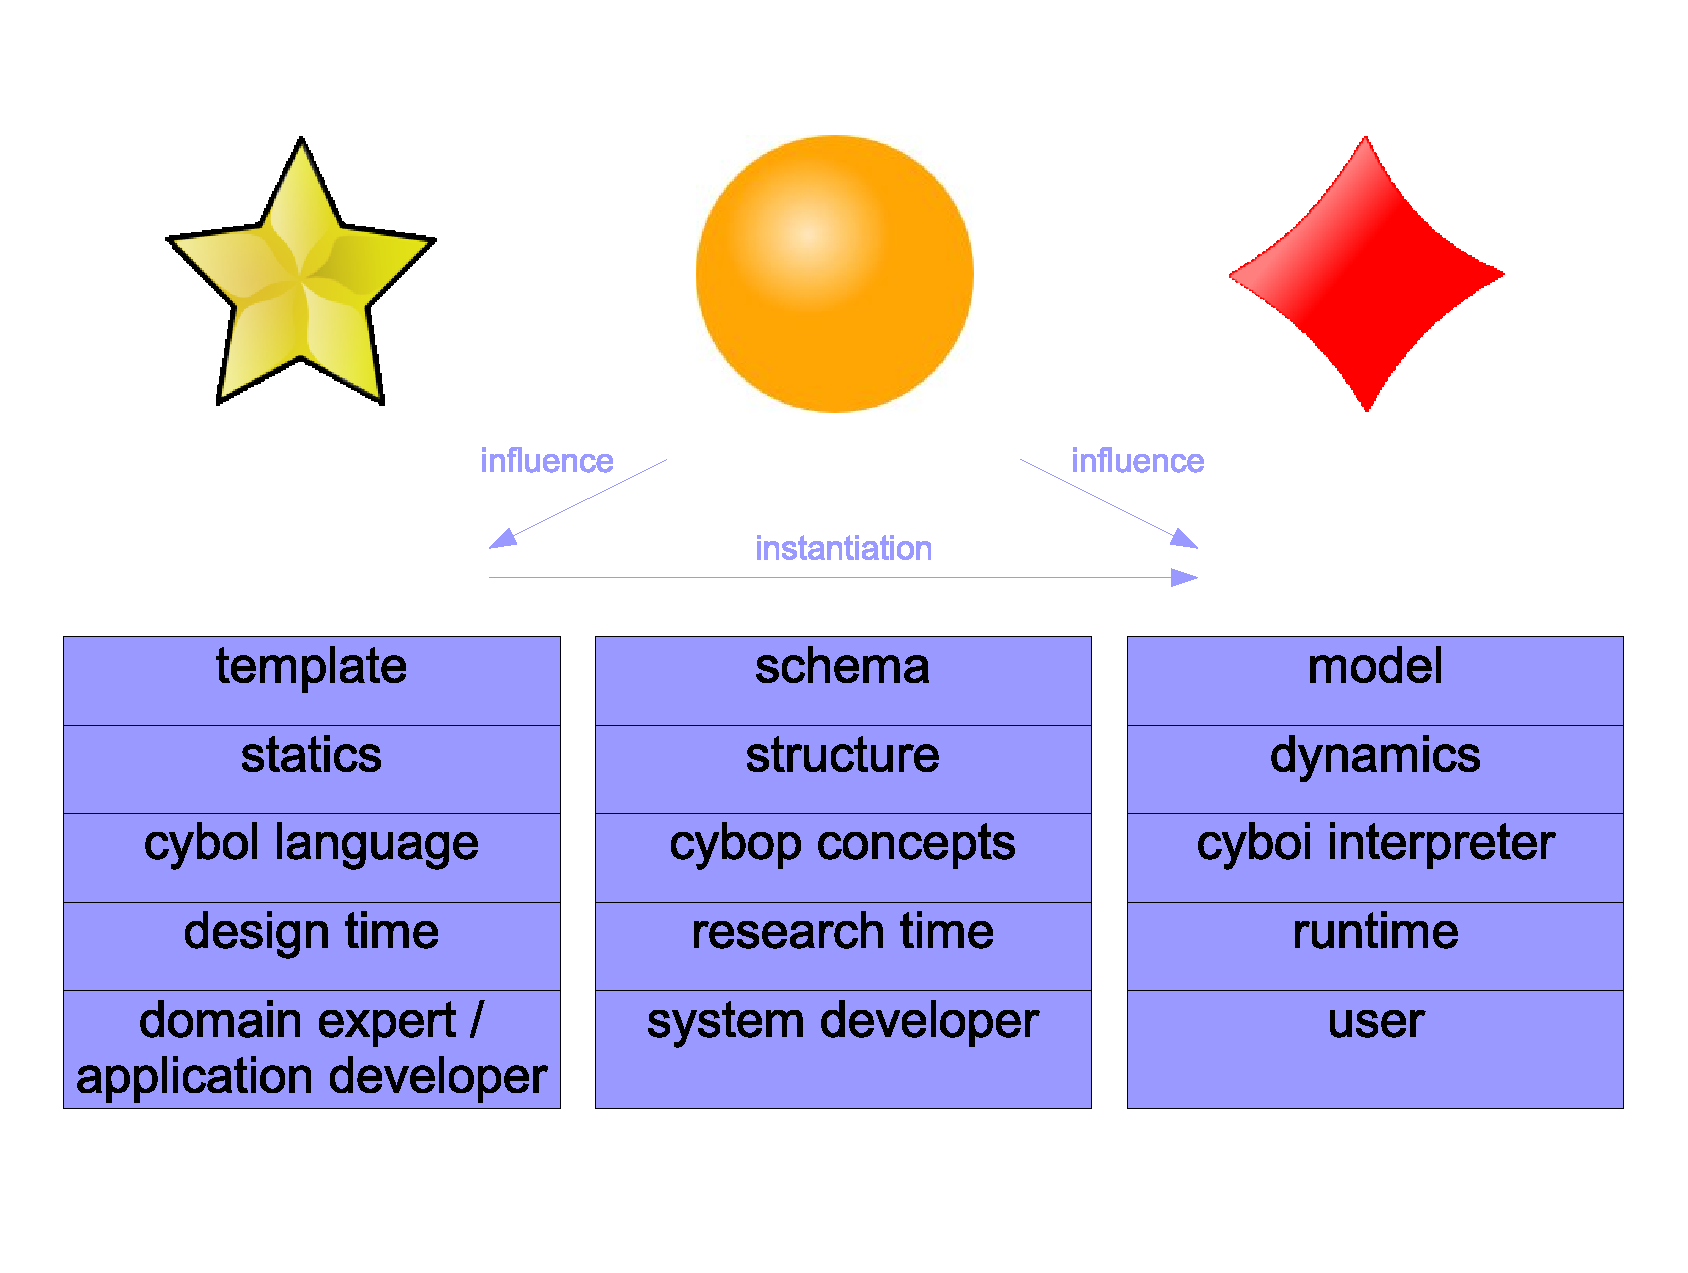
\includegraphics[scale=0.2]{vector/triumvirate.eps}
        \caption{Knowledge Triumvirate}
        \label{triumvirate_figure}
    \end{center}
\end{figure}

The results can be reduced to one illustration: the \emph{Knowledge Triumvirate}
(figure \ref{triumvirate_figure}). Its centrepiece is the new CYBOP knowledge
\emph{Schema} providing a structure to both, knowledge templates and -models.
CYBOI \emph{Models} are the dynamic runtime instances of static design-time
CYBOL \emph{Templates}.

Because all knowledge is stored in tree-form, application systems become much
more flexible than complex class networks as known from OOP. Tree structures
are easy to edit. They allow to better estimate changes caused by new
requirements, because dependencies are obvious. Software maintenance gets
improved, because application developers can focus on pure domain knowledge;
low-level system functionality is provided by CYBOI. CYBOL applications are
therefore not only portable, but represent truely long-life systems.

\begin{figure}[ht]
    \begin{center}
        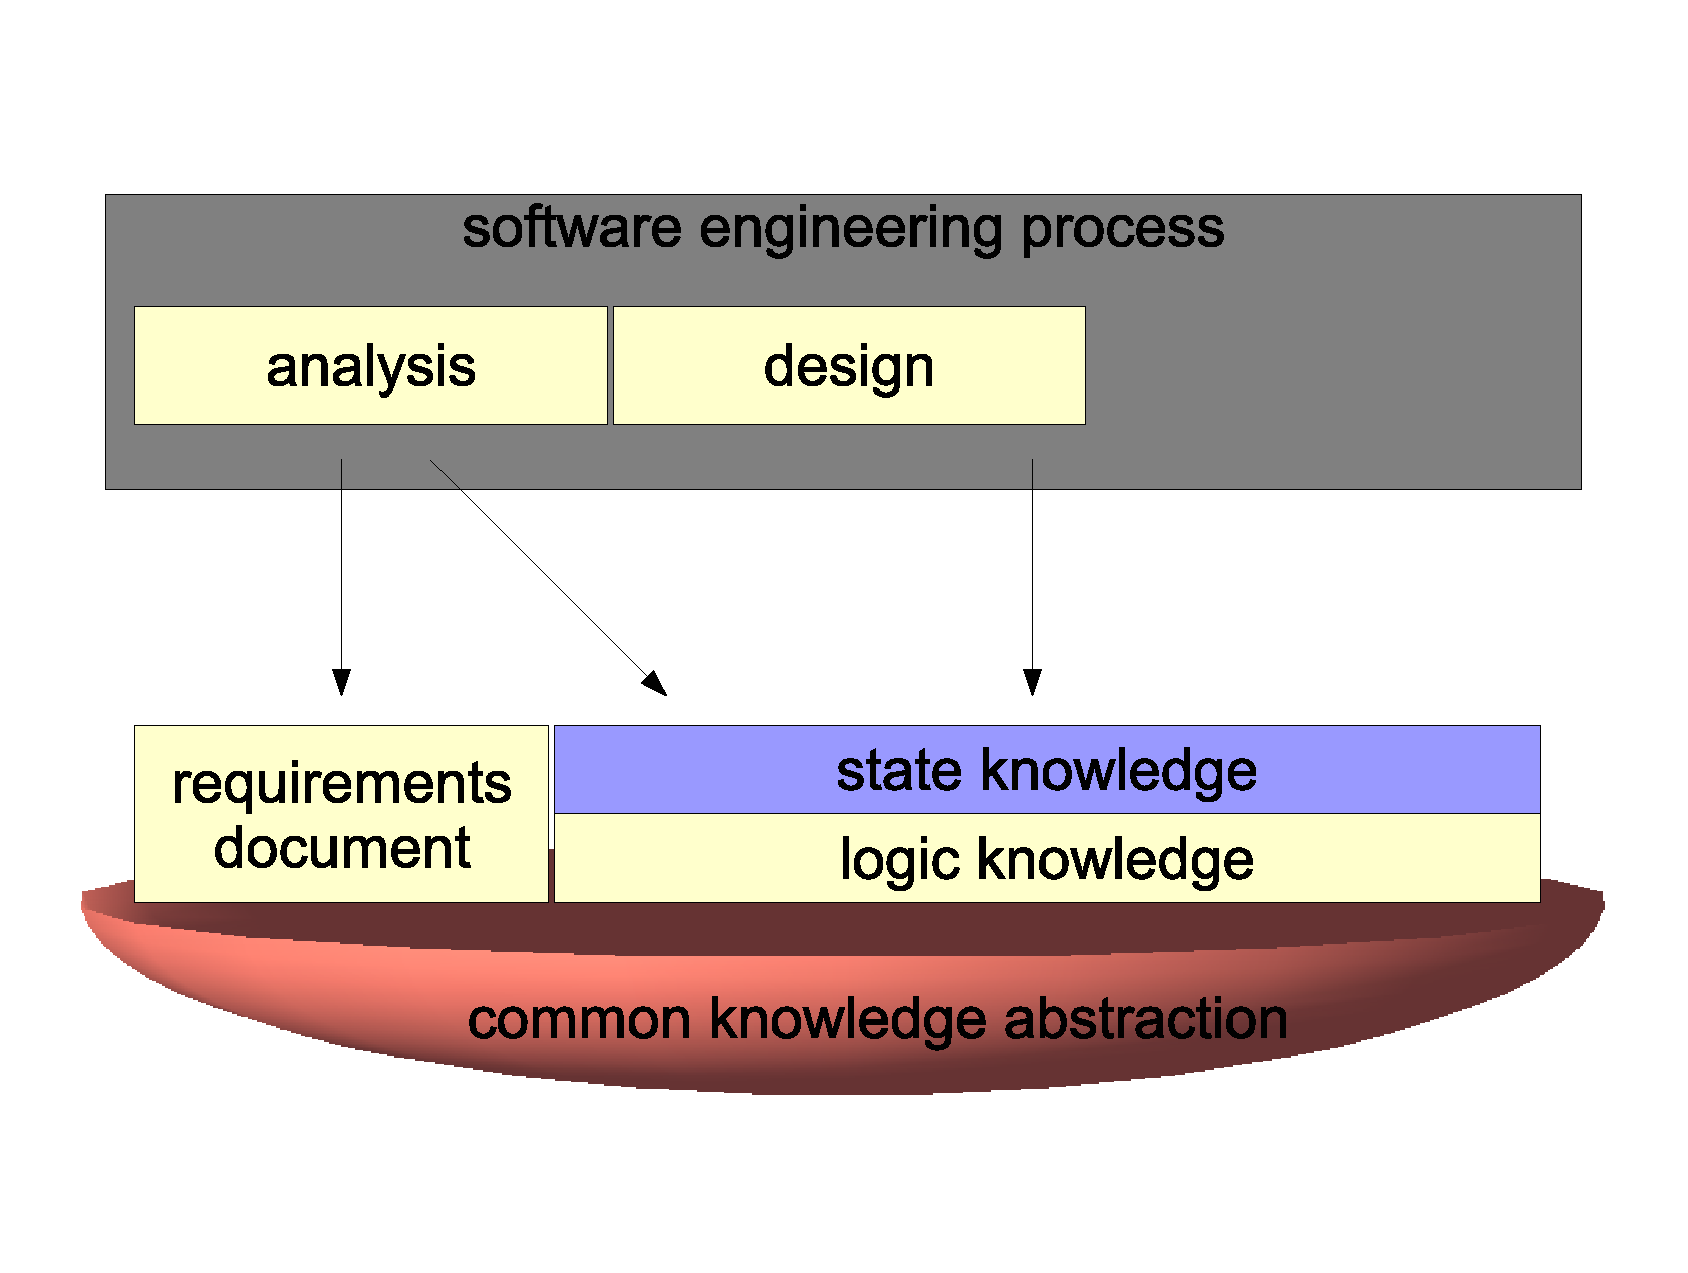
\includegraphics[scale=0.2]{vector/common.eps}
        \caption{Common Knowledge Abstraction}
        \label{common_figure}
    \end{center}
\end{figure}

Although this work does not address the \emph{Software Engineering Process}
(SEP) directly, its results have great effect on it. Section
\ref{abstraction_gaps_heading} pointed out abstraction gaps and multiple
development paradigm switches, happening during a software project's lifetime.
It set out to find a \emph{Common Knowledge Abstraction} for all phases. The
results of this work help overcome \emph{Gap 2} (figure \ref{gaps_figure}).
Since knowledge gets interpreted directly, the formerly needed implementation
phase disappears (figure \ref{common_figure}).

CYBOP applications are capable of communicating universally. CYBOI contains all
necessary mechanisms, so that it suffices to issue a \emph{send}/
\emph{receive} operation with the corresponding language, in a CYBOL template.

Naturally, there are limits to CYBOP. It does not claim to be \emph{the}
approach for all kinds of programming problems, although it thinks to
contribute suitable concepts for business application development. However, its
usability for hardware-close systems with Real Time (RT) requirements is
questionnable, as it cannot guarantee signal execution in time.

\newpage{\pagestyle{empty}\cleardoublepage}
%
% $RCSfile: appendices.tex,v $
%
% Copyright (c) 2002-2007. Christian Heller. All rights reserved.
%
% Permission is granted to copy, distribute and/or modify this document
% under the terms of the GNU Free Documentation License, Version 1.1 or
% any later version published by the Free Software Foundation; with no
% Invariant Sections, with no Front-Cover Texts and with no Back-Cover
% Texts. A copy of the license is included in the section entitled
% "GNU Free Documentation License".
%
% http://www.cybop.net
% - Cybernetics Oriented Programming -
%
% Version: $Revision: 1.2 $ $Date: 2007-08-01 13:59:00 $ $Author: christian $
% Authors: Christian Heller <christian.heller@tuxtax.de>
%

\chapter{Appendices}
\label{appendices_heading}

%
% $RCSfile: abbreviations.tex,v $
%
% Copyright (c) 2002-2007. Christian Heller. All rights reserved.
%
% Permission is granted to copy, distribute and/or modify this document
% under the terms of the GNU Free Documentation License, Version 1.1 or
% any later version published by the Free Software Foundation; with no
% Invariant Sections, with no Front-Cover Texts and with no Back-Cover
% Texts. A copy of the license is included in the section entitled
% "GNU Free Documentation License".
%
% http://www.cybop.net
% - Cybernetics Oriented Programming -
%
% Version: $Revision: 1.1 $ $Date: 2007-07-17 20:02:36 $ $Author: christian $
% Authors: Christian Heller <christian.heller@tuxtax.de>
%

%
% More abbreviations can be found at:
%
% http://www.ownnetwork.mfluhr.de/Glossar.htm
% http://www.ciw.uni-karlsruhe.de/abklex.html
% http://www.sans.org/resources/glossary.php
% http://www.cknow.com/ckinfo/acro_d/dde_1.shtml
% http://filext.com/
% http://forum.europa.eu.int/Public/irc/dsis/coded/info/data/abbreviations/en/all.htm
% http://www.sheilapantry.com/figuk/acronyms.html
% http://sir.cyivs.cy.edu.tw/~hchung/computerabbreviation.htm
% http://dmi-www.mc.duke.edu/dukemi/acronyms.htm (healthcare standards)
%

\section[Abbreviations]{Abbreviations}
\label{abbreviations_heading}

\begin{tabbing}
    \hspace{1cm} \= \hspace{2cm} -- \= \hspace{1.5cm}\= \kill

%    \>3GL \>\>Third Generation Language\\

%    \>4GL \>\>Fourth Generation Language\\

%    \>a/c \>\>account\\

%    \>a/o \>\>account of\\

%    \>a/v \>\>ad valorem (according to value)\\

%    \>AAFP \>\>American Academy of Family Physicians\\

%    \>AAP \>\>American Academy of Pediatrics\\

%    \>ABDA \>\>Bundesvereinigung Deutscher Apotheker Verbaende\\

%    \>ACAP \>\>Application Control Access Protocol\\

%    \>ACID \>\>Atomicity, Consistency, Isolation, Durability\\

%    \>ACL \>\>Access Control List\\

%    \>ACL \>\>Agent Communication Language\\

%    \>ACM \>\>Association for Computing Machinery\\

%    \>ACR \>\>American College of Radiology\\

%    \>ad fin. \>\>ad finem\\

%    \>ad inf. \>\>ad infinitem\\

%    \>ad int. \>\>ad interim\\

%    \>ad lib. \>\>ad libitum\\

%    \>ad loc. \>\>ad locum\\

%    \>AD \>\>Activity Diagram\\

%    \>ADA \>\>American Dental Association\\

%    \>ADL \>\>Archetype Definition Language\\

%    \>ADL \>\>Architecture Description Language\\

%    \>ADO \>\>ActiveX Data Object\\

%    \>ADSL \>\>Asymmetrical DSL\\

%    \>ADT \>\>Abrechnungs DT\\

%    \>AE \>\>Application Engineering\\

%    \>AE \>\>Automation Engineering\\

%    \>AGOP \>\>Agent Oriented Programming\\

%    \>AI \>\>Artificial Intelligence\\

%    \>AID \>\>Application ID\\

%    \>AIDS \>\>Anomaly-based IDS\\

%    \>ALU \>\>Arithmetic Logic Unit\\

%    \>AM \>\>Access Mode\\

%    \>AM \>\>Archetype Model\\

%    \>AMA \>\>American Medical Association\\

%    \>AMR \>\>Automated Medical Record\\

%    \>ANN \>\>Artificial Neural Network\\

%    \>ANSI \>\>American National Standards Institute\\

%    \>AODT \>\>Ambulant Operieren DT\\

%    \>AOP \>\>Aspect Oriented Programming\\

%    \>AOSD \>\>Aspect Oriented SD\\

%    \>API \>\>Application Programming Interface\\

%    \>ARP \>\>Address Resolution Protocol\\

%    \>ARQ \>\>Automatic Repeat Request\\

%    \>ARR \>\>Access Rule Reference\\

%    \>ASCII \>\>American Standard Code for Information Interchange\\

%    \>ASD \>\>Adaptive Software Development\\

%    \>ASE \>\>Application Service Element\\

%    \>ASIC \>\>Application Specific IC\\

%    \>ASN \>\>Abstract Syntax Notation\\

%    \>ASP \>\>Active Server Pages\\

%    \>ASP \>\>Application Service Provider\\

%    \>ASTM \>\>American Society for Testing and Materials\\

%    \>AT \>\>AUT Template\\

%    \>ATM \>\>Asynchronous Transfer Mode\\

%    \>ATP \>\>Appletalk Transaction Protocol\\

%    \>ATR \>\>Answer to Reset\\

%    \>AUT \>\>Authentication\\

%    \>AVI \>\>Audio Video Interleave\\

%    \>AWT \>\>Abstract Window Toolkit\\

%    \>B-ISDN \>\>Broadband ISDN\\

%    \>B2B \>\>Business to Business\\

%    \>BASIC \>\>Beginners All purpose Symbolic Instruction Code\\

%    \>B.C. \>\>before Christ\\

%    \>BCD \>\>Binary Coded Decimal\\

%    \>BCDIC \>\>BCD Interchange Code\\

%    \>BDT \>\>Behandlungs DT\\

%    \>BeOS \>\>Be, Inc. OS\\

%    \>BER \>\>Basic Encoding Rules\\

%    \>BIOS \>\>Basic I/O System\\

%    \>Bit \>\>Binary Digit\\

%    \>BLOB \>\>Binary LOB\\

%    \>BMC \>\>BioMed Central\\

%    \>BNF \>\>Backus Naur Form\\

%    \>BO \>\>Business Object\\

%    \>BOOTP \>\>BOOTstrap Protocol\\

%    \>BSD \>\>Berkeley Software (System) Distribution (Design)\\

%    \>C \>\>Certificate\\

%    \>c/o \>\>care of\\

%    \>c/s \>\>client/ server\\

%    \>C.O.D. \>\>Cash on Delivery\\

%    \>CA \>\>Certification Authority\\

%    \>CAD \>\>Computer Aided Design\\

%    \>cADL \>\>Constraint Form of ADL\\

%    \>CAM \>\>Computer Aided Manufacturing\\

%    \>CAP \>\>College of American Pathologists\\

%    \>CAPI \>\>Common ISDN Application Programming Interface\\

%    \>CAR \>\>CA Reference\\

%    \>CASE \>\>Computer Aided Software Engineering\\

%    \>CASE \>\>Common ASE\\

%    \>CBC \>\>Cipher Block Chaining\\

%    \>CBD \>\>Component Based Design (Development)\\

%    \>CBO \>\>Community Based Organisation\\

%    \>CC \>\>Cryptographic Checksum\\

%    \>CCR \>\>Continuity of Care Record\\

%    \>CCT \>\>CC Template\\

%    \>CD \>\>Certificate Directory\\

%    \>CD \>\>Collision Detection\\

%    \>CD \>\>Communication Diagram\\

%    \>CDA \>\>Clinical Document Architecture\\

%    \>CDB \>\>Check Digit Byte\\

%    \>CDDI \>\>Copper Distributed Data Interface\\

%    \>CDISC \>\>Clinical Data Interchange Standards Consortium\\

%    \>CEN \>\>Comite Europeen de Normalisation\\
%        \>\>\>(European Committee for Standardisation)\\

%    \>CENELEC \>\>CEN Electrotechnique\\
%        \>\>\>(European Committee for Electrotechnical Standardisation)\\

%    \>CEO \>\>Chief Executive Officer\\

%    \>CEPT \>\>European Conference of Post and Telecommunication Administrations\\

%    \>CERN \>\>Conseil Europeen pour le Recherche Nucleaire\\

%    \>CertSign \>\>Certificate Signing\\

%    \>CG \>\>Cryptogram\\

%    \>CGI \>\>Common Gateway Interface\\

%    \>CH \>\>Card Holder\\

%    \>CHA \>\>Certificate Holder Authorisation\\

%    \>CHR \>\>Certificate Holder Reference\\

%    \>CIAC \>\>Computer Incident Advisory Capability\\

%    \>CIAS \>\>Clinical Image Access Service\\

%    \>CICS \>\>Customer Information Control System\\

%    \>CII \>\>Computer Implemented Inventions\\

%    \>CIR \>\>Committed Information Rate\\

%    \>CISC \>\>Complex Instruction Set Computing\\

%    \>CL \>\>Common Lisp\\

%    \>CLM \>\>Connectionless Service\\

%    \>CLNP \>\>Connectionless Network Layer Protocol\\

%    \>CLNS \>\>Connectionless Network Service\\

%    \>CLOS \>\>Common Lisp Object System\\

%    \>CLSI \>\>Clinical and Laboratory Standards Institute\\

%    \>CMC \>\>Computer Mediated Communication\\

%    \>CMC \>\>Common Mail Calls\\

%    \>CmD \>\>Component Diagram\\

%    \>CMET \>\>Common Message Element Type\\

%    \>CMM \>\>Capability Maturity Model\\

%    \>CMMI \>\>Capability Maturity Model Integration\\

%    \>CMR \>\>Computerised Medical Record\\

%    \>CMS \>\>Content Management System\\

%    \>CMS \>\>Card Management System\\

%    \>CNS \>\>Central NS\\

%    \>COAS \>\>Clinical Observations Access Service\\

%    \>COBOL \>\>Common Business Oriented Language\\

%    \>CoD \>\>Communication (Collaboration) Diagram\\

%    \>COM \>\>Component Object Model\\

%    \>COM \>\>Connection-Oriented Service\\

%    \>COO \>\>Chief Operating Officer\\

%    \>COP \>\>Component Oriented Programming\\

%    \>CORBA \>\>Common ORB Architecture\\

%    \>COS \>\>Card OS\\

%    \>CP/M \>\>Control Program for Microprocessors\\
%        \>\>\>(Control Program/ Monitor)\\

%    \>CPI \>\>Certificate Profile ID\\

%    \>CPR \>\>Computer-based Patient Record\\
%        \>\>\>(Computerised Patient Record)\\

%    \>CPT \>\>Current Procedural Terminology\\

%    \>CPRI \>\>CPR Institute\\

%    \>CPRS \>\>CPR System\\

%    \>CPU \>\>Central Processing Unit\\

%    \>CR \>\>CEN Report\\

%    \>CRC \>\>Class, Responsibilities, Collaborations\\

%    \>CRC \>\>Cyclic Redundancy Check\\

%    \>CRC \>\>Cyclic Redundancy Code\\

%    \>CRM \>\>Common Reference Model\\

%    \>CS \>\>CertSign\\

%    \>CsD \>\>Class Diagram\\

%    \>CSD \>\>Composite Structure Diagram\\

%    \>CSMA \>\>Carrier Sensing Multiple Access\\

%    \>CSMA/CA \>\>Carrier Sensing Multiple Access with Collision Avoidance\\

%    \>CSMA/CD \>\>Carrier Sensing Multiple Access with Collision Detection\\

%    \>CSP \>\>Certificate Service Provider\\

%    \>CSS \>\>Cascading Style Sheet\\

%    \>CSV \>\>Comma Separated Variable\\

%    \>CT \>\>Computer Tomograph\\

%    \>CTV3 \>\>Clinical Terms Version 3\\

%    \>CVS \>\>Concurrent Versions System\\

%    \>CWA \>\>CEN Working Agreement\\

%    \>CWM \>\>Common Warehouse Metamodel\\

    \>CYBOI \>\>Cybernetics Oriented Interpreter\\

    \>CYBOL \>\>Cybernetics Oriented Language\\

%    \>CYBOM \>\>Cybernetics Oriented Methodology\\

    \>CYBOP \>\>Cybernetics Oriented Programming\\

%    \>CYBORG \>\>Cybernetic Organism\\

%    \>CYBOS \>\>Cybernetics Oriented Operating System\\

%    \>CYBOX \>\>Cybernetics Oriented Box\\

%    \>dADL \>\>Data Definition Form of ADL\\

%    \>DAG \>\>Directed Acyclic Graph\\

%    \>DAML \>\>DARPA Agent ML\\

%    \>DAO \>\>Data Access Object\\

%    \>DARPA \>\>Defense Advanced Research Projects Agency\\

%    \>DB \>\>Database\\

%    \>DB2 \>\>DB 2\\

%    \>DBMS \>\>DB Management System\\

%    \>DCC \>\>Direct Client to Client Protocol\\

%    \>DCD \>\>Document Content Description\\

%    \>DCE \>\>Distributed Computing Environment\\

%    \>DCE \>\>Data Circuit-Terminating Equipment\\
 � �%    \>\>\>(Data Communications Equipment)\\

%    \>DCL \>\>Data Control Language\\

%    \>DCOM \>\>Distributed COM\\

%    \>DD \>\>Deployment Diagram\\

%    \>DDE \>\>Dynamic Data Exchange\\

%    \>DDL \>\>Data Definition Language\\

%    \>DDoS \>\>Distributed Denial of Service\\

%    \>DDP \>\>Datagram Delivery Protocol\\

%    \>DE \>\>Domain Engineering\\

%    \>DEB \>\>Debian GNU/Linux Package\\

%    \>DES \>\>Data Encryption Standard\\

%    \>DFN \>\>Deutsches Forschungsnetz\\

%    \>DHTML \>\>Dynamic HTML\\

%    \>DICOM \>\>Digital Imaging and Communications in Medicine\\

%    \>DIF \>\>Data Interchange Format\\

%    \>DIMDI \>\>Deutsches Institut fuer Medizinische Dokumentation und Information\\

%    \>DIMSE \>\>DICOM Message Service Element\\

%    \>DIN \>\>Deutsches Institut fuer Normung\\

%    \>DIR \>\>Directory\\

%    \>DLC \>\>Dynamic Link Control\\

%    \>DLL \>\>Dynamic Link Library\\

%    \>DML \>\>Data Manipulation Language\\

%    \>DMP \>\>Disease Management Programme\\

%    \>DMR \>\>Digital Medical Record\\

%    \>DNA \>\>Desoxy Ribo Nucleic Acid\\

%    \>DNA \>\>Distributed interNet Application Architecture\\

%    \>DNR \>\>Do Not Resuscitate\\

%    \>DNS \>\>Domain Name Service\\
%        \>\>\>(Domain Name System)\\

%    \>DOM \>\>Document Object Model\\

%    \>DOS \>\>Disk OS\\

%    \>DPMI \>\>DOS Protected Mode Interface\\

%    \>DQDB \>\>Distributed Queue Dual Bus\\

%    \>DSDM \>\>Dynamic System Development Method\\

%    \>DS \>\>Digital Signature\\

%    \>DSI \>\>DS Input\\

%    \>DSL \>\>Digital Subscriber Line\\

%    \>DSL \>\>Domain Specific Language\\

%    \>DSOM \>\>Distributed System Object Model\\

%    \>DSP \>\>Digital Signal Processor\\

%    \>DSSSL \>\>Document Style Semantics and Specification Language\\

%    \>DST \>\>DS Template\\

%    \>DT \>\>Datentraeger\\

%    \>DTD \>\>Document Type Definition\\

%    \>DTE \>\>Data Termination Equipment\\

%    \>DTO \>\>Data Transfer Object\\

%    \>DVI \>\>Device Independent\\

%    \>DVI \>\>Digital Video Interface\\

%    \>e.g. \>\>exempli gratia (for example)\\

%    \>EAA \>\>Enterprise Application Architecture\\

%    \>EBCDIC \>\>Extended BCDIC\\

%    \>EBES \>\>European Board of EDI Standardisation\\

%    \>EBNF \>\>Extended BNF\\

%    \>EC \>\>Existential Conjunctive\\

%    \>ECC \>\>Error Correction Code\\
%        \>\>\>(Error Checking and Correction)\\

%    \>ECML \>\>Electronic Commerce Modeling Language\\

%    \>ED \>\>Emergency Department\\

%    \>EDI \>\>Electronic Data Interchange\\

%    \>EDIF \>\>EDI Format\\

%    \>EDIFACT \>\>EDI for Administration, Commerce and Transport\\

%    \>EDP \>\>Electronic Data Processing\\

%    \>EEG \>\>EBES Expert Group\\

%    \>EEPROM \>\>Electrically Erasable Programmable ROM\\

%    \>EET \>\>Encyclopedia of Educational Technology\\

%    \>EGP \>\>Exterior Gateway Protocol\\

%    \>eHC \>\>Electronic Health Card\\

%    \>EHCR \>\>Electronic Health Care Record\\

%    \>EHR \>\>Electronic Health Record\\

%    \>EHRcom \>\>EHR Communications\\

%    \>EIA \>\>Electronic Industries Alliance\\

%    \>EICAR \>\>European Institute for Computer Anti-Virus Research\\

%    \>EIR \>\>Electronic Insurance Record\\

%    \>EJB \>\>Enterprise Java Bean\\

%    \>EMA \>\>Electronic Messaging Association\\

%    \>EMI \>\>Electronic Medical Infrastructure\\

%    \>EMR \>\>Electronic Medical Record\\

%    \>EN \>\>European Standard\\

%    \>ENV \>\>European Prestandard\\

%    \>EOF \>\>End of File\\

%    \>EPR \>\>Electronic Patient Record\\

%    \>EPS \>\>Encapsulated PS\\

%    \>ER \>\>Endoplasmic Reticulum\\

%    \>ERD \>\>Entity Relationship Diagram\\

%    \>ERM \>\>Entity Relationship Model\\

%    \>ERP \>\>Enterprise Resource Planning\\

%    \>et al. \>\>et alii (and others)\\

%    \>etc. \>\>et cetera (and so on)\\

%    \>ETH \>\>Eidgenoessische Technische Hochschule\\

%    \>ETSI \>\>European Telecommunications Standards Institute\\

%    \>EU \>\>European Union\\

%    \>EUD \>\>End User Development\\

%    \>Extended ML \>\>Extended Meta Language\\

%    \>FAQ \>\>Frequently Asked Question\\

%    \>FAX \>\>Facsimile Transmission\\

%    \>FBO \>\>Faith Based Organisation\\

%    \>FDD \>\>Feature Driven Development\\

%    \>FDDI \>\>Fiber Distributed Data Interface\\

%    \>FDL \>\>Free Documentation License\\

%    \>FeatuRSEB \>\>Feature RSEB\\

%    \>FEC \>\>Forward Error Correction\\

%    \>FHS \>\>Filesystem Hierarchy Standard\\

%    \>FIC \>\>Family of International Classifications\\

%    \>FIFO \>\>First In, First Out\\

%    \>FLOSS \>\>Free/ Libre OSS\\

%    \>FODA \>\>Feature Oriented Domain Analysis\\

%    \>FOLDOC \>\>Free On-line Dictionary of Computing\\

%    \>FOPL \>\>First Order Predicate Logic\\

%    \>FORE \>\>Family Oriented Requirements Engineering\\

%    \>FOSS \>\>Free and OSS\\

%    \>FPGA \>\>Field Programmable Gate Array\\

%    \>FPU \>\>Floating Point Unit\\

%    \>FQN \>\>Fully Qualified Name\\

%    \>FR \>\>Frame Relay\\

%    \>FRAD \>\>FR Access Device\\

%    \>FSF \>\>Free Software Foundation\\

%    \>FTAM \>\>File Transfer, Access and Management\\

%    \>FTP \>\>File Transfer Protocol\\

%    \>GA \>\>Genetic Algorithm\\

%    \>GALEN \>\>Generalised Architecture for Languages,\\
%        \>\>\>Encyclopaedias and Nomenclatures in Medicine\\

%    \>GAN \>\>Global Area Network\\

%    \>GC \>\>Garbage Collector\\

%    \>GCC \>\>GNU�Compiler Collection\\
%        \>\>\>(GNU C�Compiler)\\

%    \>GDI \>\>Graphics Device Interface\\

%    \>GDT \>\>Geraete DT\\

%    \>GEHR \>\>Good European/ EHR\\

%    \>GEMATIK \>\>Gesellschaft fuer Telematikanwendungen der Gesundheitskarte\\

%    \>GGP \>\>Gateway-to-Gateway Protocol\\

%    \>GIF \>\>Graphics Interchange Format\\

%    \>GIMP \>\>General (GNU) Image Manipulation Program\\

%    \>GMDN \>\>Global Medical Device Nomenclature\\

%    \>GNOME \>\>GNU Network Object Model Environment\\

%    \>GNU \>\>GNU is not UNIX\\

%    \>GoF \>\>Gang of Four\\

%    \>GP \>\>Generative Programming\\

%    \>GP \>\>General Practitioner\\

%    \>GPF \>\>General Protection Fault\\

%    \>GPIC \>\>General Purpose Information Component\\

%    \>GPL \>\>General Public License\\

%    \>GPL \>\>General Purpose Language\\

%    \>GPS \>\>Global Positioning System\\

%    \>GRAIL \>\>GALEN Representation and Integration Language\\

%    \>GTK \>\>GIMP Toolkit\\

%    \>GUI \>\>Graphical UI\\

%    \>GUID \>\>Globally Unique ID\\

%    \>h/w \>\>Hardware\\

%    \>HAL \>\>Hardware Abstraction Layer\\

%    \>HBCI \>\>Homenanking Computer Interface\\

%    \>HCI \>\>Human-Computer Interaction\\

%    \>HD \>\>Harmonisation Document\\

%    \>HDD \>\>Hard Disk Drive\\

%    \>HDL \>\>Hardware Description Language\\

%    \>HDLC \>\>High level Data Link Control\\

%    \>HDTF \>\>Healthcare Domain Task Force\\

%    \>HIDS \>\>Host based IDS\\

%    \>HIMSS \>\>Health Information Management and Systems Society\\

%    \>HIPAA \>\>Healthcare Insurance Portability and Accountability Act\\

%    \>HIS \>\>Hospital Information System\\

%    \>HL7 \>\>Health Level Seven\\

%    \>HMVC \>\>Hierarchical MVC\\

%    \>HOWTO \>\>How To? (Subject Specific Help)\\

%    \>HP \>\>Hewlett Packard\\

%    \>HPC \>\>Health Professional Card\\

%    \>HPTC \>\>High Performance Technical Computing\\

%    \>HTML \>\>Hypertext ML\\

%    \>HTTP \>\>Hypertext Transfer Protocol\\

%    \>HTTP-ng \>\>HTTP next generation\\

%    \>HTTPD \>\>HTTP Daemon\\

%    \>HTTPS \>\>HTTP over SSL\\

%    \>HUK \>\>Haftpflicht-Unterstuetzungs-Kasse Coburg\\

%    \>HW \>\>Hardware\\

%    \>HXP \>\>Healthcare Xchange Protocol\\

%    \>i/e \>\>import/ export\\

%    \>i/o \>\>input/ output\\

%    \>i/p \>\>input\\

%    \>IABG \>\>Industrieanlagen-Betriebsgesellschaft\\

%    \>ib. \>\>ibidem (in the same place)\\

%    \>ibid. \>\>ib.\\

%    \>IBM \>\>International Business Machines\\

%    \>i/c \>\>in charge of\\

%    \>IC \>\>Integrated Circuit\\

%    \>ICC \>\>IC Card\\

%    \>ICCSN \>\>ICC SN\\

%    \>ICANN \>\>Internet Corporation for Assigned Names and Numbers\\

%    \>ICD \>\>International Classification of Diseases\\

%    \>ICF \>\>International Classification of Functioning, Disability and Health\\

%    \>ICHI \>\>International Classification of Health Interventions\\

%    \>ICHPPC \>\>International Classification of Health Problems in Primary Care\\

%    \>ICMP \>\>Internet Control Message Protocol\\

%    \>ICN \>\>International Council of Nurses\\

%    \>ICNP \>\>International Classification for Nursing Practice (Procedures)\\

%    \>ICQ \>\>I seek you\\

%    \>ICR \>\>Integrated Care Record\\

%    \>ICPC \>\>International Classification of Primary Care\\

%    \>id. \>\>idem (the same)\\

%    \>ID \>\>Identifier\\

%    \>IDE \>\>Integrated Development Environment\\

%    \>IDEA \>\>International Data Encryption Algorithm\\

%    \>IDL \>\>Interface Definition Language\\

%    \>IDS \>\>Intrusion Detection System\\

%    \>i.e. \>\>id est (that is)\\

%    \>IEEE \>\>Institute of Electrical and Electronics Engineers\\

%    \>IETF \>\>Internet Engineering Task Force\\

%    \>IGMP \>\>Internet Group Management Protocol\\

%    \>IGP \>\>Interior Gateway Protocol\\

%    \>IIIS \>\>International Institute of Informatics and Systemics\\

%    \>IIM \>\>Internet Interaction Management\\

%    \>IIOP \>\>Internet Inter ORB Protocol\\

%    \>IIS \>\>Internet Information Server\\

%    \>IM \>\>Information Model\\

%    \>IMAP \>\>Internet Message Access Protocol\\

%    \>IMP \>\>Interface Message Processor\\

%    \>IMTC \>\>International Multimedia Teleconferencing Consortium\\

%    \>Inc. \>\>Incorporated\\

%    \>InterNIC \>\>Internet Network Information Center\\

%    \>IoC \>\>Inversion of Control\\

%    \>IOD \>\>Interaction Overview Diagram\\

%    \>IOM \>\>Institute of Medicine\\

%    \>IP \>\>Internet Protocol\\

%    \>IPC \>\>Inter-Process Communication\\

%    \>IPv6 \>\>Internet Protocol (Version 6)\\

%    \>IPX \>\>Internet Packet Exchange\\

%    \>IRC \>\>Internet Relay Chat\\

%    \>IRQ \>\>Interrupt Request\\

%    \>IS \>\>International Standard\\

%    \>ISA \>\>Instruction Set Architecture\\

%    \>ISBD \>\>International Standard Book Description\\

%    \>ISDN \>\>Integrated Services Digital Network\\

%    \>ISO \>\>International Organization for Standardization\\

%    \>ISP \>\>Internet Service Provider\\

%    \>IST \>\>Information Science Technology\\

%    \>IT \>\>Information Technology\\

%    \>ITC \>\>MIT Internet \& Telecoms Convergence Consortium\\

%    \>ITU \>\>International Telecommunication Union\\

%    \>J2EE \>\>Java 2 Platform Enterprise Edition\\

%    \>JAR \>\>Java Archive\\

%    \>JDBC \>\>Java DB Connectivity\\

%    \>JDK \>\>Java Development Kit\\

%    \>JEDEC \>\>Joint Electron Device Engineering Council\\

%    \>JFC \>\>Java Foundation Classes\\

%    \>JMS \>\>Java Message Service\\

%    \>JNDI \>\>Java Naming and Directory Interface\\

%    \>JNI \>\>Java Native Interface\\

%    \>JOSMC \>\>Journal of Free and Open Source Medical Computing\\

%    \>JPE \>\>Java Platform for the Enterprise\\

%    \>JPEG \>\>Joint Photographic Experts Group\\

%    \>JPM \>\>Join Point Model\\

%    \>jr. \>\>junior\\

%    \>JSP \>\>Java Server Pages\\

%    \>JTM \>\>Job Transfer and Management (Manipulation)\\

%    \>JTS \>\>Java Transaction Service\\

%    \>JVM \>\>Java VM\\

%    \>KBV \>\>Kassenaerztliche Bundesvereinigung\\

%    \>KDE \>\>K Desktop Environment\\

%    \>KDT \>\>Kommunikations DT\\

%    \>KE \>\>Knowledge Engineering\\

%    \>KE \>\>Key Encipherment\\

%    \>KEI \>\>KE Input\\

%    \>KID \>\>Key ID\\

%    \>KIF \>\>Knowledge Interchange Format\\

%    \>KIS \>\>Krankenhaus Informations System\\

%    \>KMU \>\>Kleines oder Mittelst\"andisches Unternehmen\\

%    \>KQML \>\>Knowledge Query and Manipulation Language\\

%    \>KV \>\>Kassenaerztliche Vereinigung\\

%    \>KVDT \>\>KV DT\\

%    \>l.c. \>\>loco citato (in the place cited)\\

%    \>L2F \>\>Layer 2 Forwarding\\

%    \>L2TP \>\>Layer 2 Tunneling Protocol\\

%    \>LAN \>\>Local Area Network\\

%    \>LAMP \>\>Linux, Apache, MySQL, PHP/ Perl/ Python\\

%    \>LAMPS \>\>LAMP and SSL\\

%    \>LAPB \>\>Link Access Procedure balanced\\

%    \>LAPD \>\>Link Access Procedure D-channel\\

%    \>LAPM \>\>Link Access Procedure for Modems\\

%    \>LaTeX \>\>Lamport TeX\\

%    \>LDAP \>\>Lightweight Directory Access Protocol\\

%    \>LDR \>\>Lifetime Data Repository\\

%    \>LDT \>\>Labor DT\\

%    \>LGPL \>\>Lesser GPL\\

%    \>LIFO \>\>Last In, First Out\\

%    \>LILO \>\>Linux Loader\\

%    \>LLC \>\>Logical Link Control\\

%    \>LOB \>\>Large Object\\

%    \>LOINC \>\>Logical Observation Identifiers, Names and Codes\\

%    \>LQS \>\>Lexicon (Terminology) Query Service\\

%    \>LRC \>\>Longitudinal Redundancy Check\\

%    \>LSB \>\>Least Significant Byte\\

%    \>Ltd. \>\>limited\\

%    \>LTM \>\>Long Term Memory\\

%    \>LUG \>\>Linux User Group\\

%    \>M. Sc. \>\>Master of Science\\

%    \>MAC \>\>Media Access Control\\

%    \>MAN \>\>Metropolitan Area Network\\

%    \>MAPI \>\>Message Application Programming Interface\\

%    \>MAS \>\>Multi Agent System\\

%    \>MathML \>\>Mathematical ML\\

%    \>MATLAB \>\>Matrix Laboratory\\

%    \>MBR \>\>Master Boot Record\\

%    \>MD \>\>Model Diagram\\

%    \>MD \>\>Medical Doctor\\

%    \>MDA \>\>Model Driven Architecture\\

%    \>MDI \>\>Multiple Document Interface\\

%    \>MeSH \>\>Medical Subject Headings\\

%    \>MFC \>\>MS Foundation Classes\\

%    \>MIF \>\>Management Information Format\\

%    \>MIME \>\>Multipurpose Internet Mail Extension\\

%    \>MIS \>\>Management Information System\\

%    \>MIT \>\>Massachusetts Institute of Technology\\

%    \>ML \>\>Markup Language\\

%    \>MMS \>\>Massachusetts Medical Society\\

%    \>MMU \>\>Memory Management Unit\\

%    \>MOF \>\>Meta Object Facility\\

%    \>MOP \>\>Meta Object Protocol\\

%    \>MOTIS \>\>Message-Oriented Text Interchange Systems\\

%    \>MPEG \>\>Moving Picture Experts Group\\
%        \>\>\>(Motion Picture Expert Group)\\

%    \>MPI \>\>Message Passing Interface\\

%    \>MPI \>\>Master Patient Index\\

%    \>MPOA \>\>Multiprotocol over ATM\\

%    \>Mr. \>\>Mister\\

%    \>Mrs. \>\>Mistress\\

%    \>MRPT \>\>Management Resource Planning Tool\\

%    \>MS \>\>Microsoft\\

%    \>MSB \>\>Most Significant Byte\\

%    \>MTP \>\>Message Transfer Protocol\\

%    \>MTU \>\>Maximum Transmission Unit\\

%    \>MUD \>\>Multi User Dungeon\\

%    \>Mutex \>\>Mutual Exclusion\\

%    \>MVC \>\>Model View Controller\\

%    \>MVS \>\>Multiple Virtual Storage\\

%    \>n/a \>\>not applicable\\

%    \>n/a \>\>no account (on cheques)\\

%    \>n.d. \>\>not dated\\

%    \>NAT \>\>Network Adress Translation\\

%    \>NC \>\>Network Computer\\

%    \>NCCLS \>\>National Committee for Clinical Laboratory Standards\\

%    \>NCPDP \>\>National Council for Prescription Drug Programs\\

%    \>NEMA \>\>National Electrical Manufacturers Association\\

%    \>NETBEUI \>\>NetBIOS Extended UI\\

%    \>NetBIOS \>\>Network BIOS\\

%    \>NetDDE \>\>Network DDE\\

%    \>NFS \>\>Network File System\\

%    \>NGI \>\>Next Generation Internet\\

%    \>NGO \>\>Non-Governmental Organisation\\

%    \>NHS \>\>National Health Service\\

%    \>NHSIA \>\>NHS Information Authority\\

%    \>NID \>\>Namespace Identifier\\

%    \>NIDS \>\>Network-based IDS\\

%    \>NIS \>\>Network Information Service\\

%    \>NIST \>\>National Institute of Standards and Technology\\

%    \>NLM \>\>National Library of Medicine\\

%    \>NNTP \>\>Network News Transfer Protocol\\

%    \>NOS \>\>Network OS\\

%    \>NPO \>\>Non-Profit Organisation\\

%    \>NS \>\>Nervous System\\

%    \>NSA \>\>National Security Agency\\

%    \>NSF \>\>National Science Foundation\\

%    \>NSP \>\>Network Service Provider\\

%    \>NSS \>\>Namespace Specific String\\

%    \>NTP \>\>Network Time Protocol\\

%    \>o/a \>\>on account of\\

%    \>o/o \>\>p.c.\\

%    \>o/p \>\>output\\

%    \>OASIS \>\>Organization for the Advancement of Structured Information Standards\\

%    \>ObD \>\>Object (Instance) Diagram\\

%    \>OCL \>\>Object Constraint Language\\

%    \>OCX \>\>OLE Custom Control\\

%    \>OD \>\>Organisation Diagram\\

%    \>ODBC \>\>Open DB Connectivity\\

%    \>ODI \>\>Open Datalink Interface\\

%    \>ODL \>\>Object Description Language\\

%    \>ODM \>\>Operational Data Modeling\\

%    \>ODP \>\>Open Distributed Processing\\

%    \>OFFIS \>\>Oldenburger Forschungs- und Entwicklungsinstitut\\
%        \>\>\>fuer Informatik-Werkzeuge und -Systeme\\

%    \>OGG \>\>Ogg Vorbis Audio Encoding and Streaming Technology\\

%    \>OID \>\>Object ID\\

%    \>OIM \>\>Open Information Model\\

%    \>OIO \>\>Open Infrastructure for Outcomes\\

%    \>OLE \>\>Object Linking and Embedding\\

%    \>OM \>\>Object Model\\

%    \>OMA \>\>Object Management Architecture\\

%    \>OMG \>\>Object Management Group\\

%    \>OMS \>\>Object Model System\\

%    \>OO \>\>Object Oriented\\
%        \>\>\>(Object Orientation)\\

%    \>OOA \>\>OO Analysis\\

%    \>OOD \>\>OO Design\\

%    \>OODBMS \>\>OO DBMS\\

%    \>OOM \>\>OO Model\\

%    \>OOP \>\>OO Programming\\

%    \>OOPS \>\>OO Programming System\\

%    \>OPCS \>\>Office of Population Censuses and Surveys\\
%        \>\>\>Classification of Surgical Operations and Procedures\\

%    \>OPD \>\>Object Process Diagram\\

%    \>OpenEHR \>\>Open EHR\\

%    \>OPS \>\>Official Production System\\

%    \>OQL \>\>Object Query Language\\

%    \>ORB \>\>Object Request Broker\\

%    \>ORDBMS \>\>Object Relational DBMS\\

%    \>OS \>\>Operating System\\

%    \>OSCAR \>\>Open Source Clinical Application Resource\\

%    \>OSDN \>\>Open Source Development Network\\

%    \>OSF \>\>Open Software Foundation\\

%    \>OSHCA \>\>Open Source Health Care Alliance\\

%    \>OSI \>\>Open Source Initiative\\

%    \>OSI \>\>Open Systems Interconnection\\

%    \>OSPF \>\>Open Shortest Path First\\

%    \>OSS \>\>Open Source Software\\

%    \>OTW \>\>Object Technology Workbench\\

%    \>OWiS \>\>Objektorientierte und Wissensbasierte Systeme\\

%    \>OWL \>\>Web Ontology Language\\

%    \>OXMIS \>\>Oxford Medical Information System\\

%    \>p.c. \>\>per cent (%)\\

%    \>P2P \>\>Peer to Peer\\
%        \>\>\>(Person-to-Person, Program-to-Program)\\

%    \>P3P \>\>Platform for Privacy Preferences Project\\

%    \>PACS \>\>Picture Archiving and Communication System\\

%    \>PAD \>\>Protocol Assembler Disassembler\\

%    \>PAN \>\>Personal Area Network\\

%    \>PAP \>\>Password Authentication Protocol\\

%    \>PBM \>\>Packet Based Network\\

%    \>PC \>\>Personal Computer\\

%    \>PCL \>\>Printer Control Language\\

%    \>PCMCIA \>\>PC Memory Card International Association\\

%    \>PCR \>\>Patient Carried Record\\

%    \>PCRF \>\>Patient Care Referral Form\\

%    \>PD \>\>Package Diagram\\

%    \>PDA \>\>Personal Digital Assistant\\

%    \>PDF \>\>Portable Document Format\\

%    \>PDL \>\>Page Description Language\\

%    \>PDU \>\>Protocol Data Unit\\

%    \>PEM \>\>Privacy Enhanced Mail\\

%    \>p.ann. \>\>per annum (yearly)\\

%    \>Perl \>\>Practical Extraction and Report Language\\

%    \>PGP \>\>Pretty Good Privacy\\

%    \>PHAGRO \>\>Bundesverband des pharmazeutischen Groszhandels\\

%    \>PhD \>\>Philosophiae Doctor\\

%    \>PHP \>\>PHP Hypertext Preprocessor\\
%        \>\>\>(Personal Home Page)\\

%    \>PHP \>\>Personal Health Project\\

%    \>PHR \>\>Personal Health Record\\

%    \>PIC \>\>Programmable Interrupt Controller\\

%    \>PICS \>\>Platform for Internet Content Selection\\

%    \>PIDS \>\>Person (Patient) Identification Service\\

%    \>PIM \>\>Platform Independent Model\\

%    \>PIM \>\>Personal Information Manager\\

%    \>PIN \>\>Personal Identification Number\\

%    \>PIO \>\>Programmed Input Output\\

%    \>Pixel \>\>Picture Element\\

%    \>PK \>\>Public Key\\

%    \>PKI \>\>PK Infrastructure\\

%    \>PL/1 \>\>Programming Language One\\

%    \>PLD \>\>Programmable Logic Device\\

%    \>PMR \>\>Patient Medical Record\\

%    \>PMS \>\>Practice Management System\\

%    \>PNG \>\>Portable Network Graphics\\

%    \>PnP \>\>Plug and Play\\

%    \>PNS \>\>Peripheral NS\\

%    \>POA \>\>Portable Object Adapter\\

%    \>POL \>\>Problem Oriented Language\\

%    \>POMR \>\>Problem Oriented Medical Record\\

%    \>POP \>\>Post Office Protocol\\

%    \>POSIX \>\>Portable OS Interface for UNIX\\

%    \>pp. \>\>pages\\

%    \>PPC \>\>Power PC\\

%    \>PPP \>\>Point-to-Point Protocol\\

%    \>PPTP \>\>Point-to-Point Tunneling Protocol\\

%    \>PrK \>\>Private Key\\

%    \>pro tem. \>\>pro tempore (for the time)\\

%    \>Prolog \>\>Programmation en Logique\\

%    \>PS \>\>PostScript\\

%    \>PSM \>\>Platform Specific Model\\

%    \>PURL \>\>Persistent URL\\

%    \>PVC \>\>Permanent Virtual Circuit\\

%    \>q.e. \>\>quod est (which is)\\

%    \>q.e.d. \>\>quod erat demonstrandum (which was to be proved)\\

%    \>q.v. \>\>quod vide (which see)\\

%    \>QMS \>\>Qualitaetsring Medizinische Software\\

%    \>QoS \>\>Quality of Service\\

%    \>Qt \>\>Cute C++ Toolkit\\

%    \>r/t \>\>radio-telegraphy\\

%    \>R.V. \>\>revised version\\

%    \>RAD \>\>Rapid Application Development\\

%    \>RADS \>\>Resource Access Decision Service\\

%    \>RAM \>\>Random Access Memory\\

%    \>RARP \>\>Reverse Address Resolution Protocol\\

%    \>RAS \>\>Remote Access Service\\

%    \>RAS \>\>Reliability, Availability, Serviceability\\

%    \>RDBMS \>\>Relational DBMS\\

%    \>RDF \>\>Resource Description Framework\\

%    \>RDS \>\>Resolver Discovery Service\\

%    \>READ \>\>Read Codes\\

%    \>RF \>\>Radio Frequency\\

%    \>RFC \>\>Request for Comment\\

%    \>RFP \>\>Request for Proposal\\

%    \>RIM \>\>Reference Information Model\\

%    \>RIP \>\>Routing Information Protocol\\

%    \>RIS \>\>Radiology Information System\\

%    \>RISC \>\>Reduced Instruction Set Computing\\

%    \>RKI \>\>Robert Koch Institut\\

%    \>RM \>\>Reference Model\\

%    \>RMI \>\>Remote Method Invocation\\

%    \>RMIM \>\>Refined Message Information Model\\

%    \>RNA \>\>Ribo Nucleic Acid\\

%    \>RND \>\>Random Number\\

%    \>ROM \>\>Read Only Memory\\

%    \>RPC \>\>Remote Procedure Call\\

%    \>RPM \>\>RPM/ Red Hat Package Manager\\

%    \>RSEB \>\>Reuse driven Software Engineering Business\\

%    \>RSP \>\>Resource Reservation Protocol\\

%    \>RSVP \>\>Resource Reservation Setup Protocol\\

%    \>RT \>\>Real Time\\

%    \>RTCP \>\>RT Control Protocol\\

%    \>RTE \>\>Roundtrip Engineering\\

%    \>RTF \>\>Rich Text Format\\

%    \>RTP \>\>RT Protocol\\

%    \>RTTI \>\>Run Time Type Identification\\

%    \>RTZ \>\>Return To Zero\\

%    \>RUP \>\>Rational Unified Process\\

%    \>s.v. \>\>sub voce (under the word)\\

%    \>S/MIME \>\>Secure MIME\\

%    \>s/w \>\>software\\

%    \>SAN \>\>Storage Area Network\\

%    \>SAS \>\>Statistical Analysis System\\

%    \>SANS \>\>System Administration, Networking and Security Institute\\

%    \>SASE \>\>Specific ASE\\

%    \>SAX \>\>Simple API for XML\\

%    \>SC \>\>Subcommittee\\

%    \>SCD \>\>State Chart Diagram\\

%    \>SCDI \>\>Standards Committee on Dental Informatics\\

%    \>SCIPHOX \>\>Standardisation of Communication between Information Systems\\
%        \>\>\>in Physician's Offices and Hospitals using XML\\

%    \>SCN \>\>Switched Circuit Network\\

%    \>SD \>\>Software Development\\

%    \>SD \>\>Sequence Diagram\\

%    \>SDK \>\>System Development Kit\\

%    \>SDL \>\>Specification and Description Language\\

%    \>SDLC \>\>Synchronous Data Link Control\\

%    \>SDM \>\>Submission Data Modeling\\

%    \>SDO \>\>Standards Development Organisation\\

%    \>SDU \>\>Service Data Unit\\

%    \>SEP \>\>Software Engineering Process\\

%    \>SEQUEL \>\>Structured English Query Language\\

%    \>SET \>\>Secure Electronic Transaction\\

%    \>SG \>\>Secretary General\\

%    \>SGB \>\>Sozialgesetzbuch\\

%    \>SGI \>\>Silicon Graphics, Inc.\\

%    \>SGML \>\>Standard Generalized ML\\

%    \>SHTTP \>\>Secure HTTP\\

%    \>SID \>\>Security ID\\

%    \>SIG \>\>Signature\\

%    \>SIG \>\>Special Interest Group\\

%    \>SK \>\>Secret Key\\

%    \>SKA \>\>Sender Keep All\\

%    \>SL \>\>Specification Language\\

%    \>SLIP \>\>Serial Line Internet Protocol\\

%    \>SM \>\>Secure Messaging\\

%    \>SMB \>\>Server Message Block\\

%    \>SMD \>\>State Machine (Chart) Diagram\\

%    \>SME \>\>Small- and Medium Sized Enterprise\\

%    \>SMIF \>\>Stream based Model Interchange Format\\

%    \>SMK \>\>SM Key\\

%    \>SMP \>\>Symmetric Multiprocessing\\
%        \>\>\>(Shared Memory Processing)\\

%    \>SMTP \>\>Simple Mail Transfer Protocol\\

%    \>SN \>\>Serial Number\\

%    \>SNA \>\>Systems Network Architecture\\

%    \>SNAP \>\>SubNetwork Access Protocol\\

%    \>SNMP \>\>Simple Network Management Protocol\\

%    \>SNOMED \>\>Systematized Nomenclature of Medicine\\

%    \>SNOMED CT \>\>SNOMED Clinical Terms\\

%    \>SNOMED RT \>\>SNOMED Reference Terminology\\

%    \>SNR \>\>Signal to Noise Ratio\\

%    \>SOA \>\>Service Oriented Architecture\\

%    \>SOAP \>\>Simple Object Access Protocol\\

%    \>SOAP \>\>Subjective, Objective, Assessment, Plan\\

%    \>SoC \>\>Separation of Concerns\\

%    \>SONET \>\>Synchronous Optical Network\\

%    \>SOP \>\>Script Oriented Programming\\

%    \>SOX \>\>Schema for Object Oriented XML\\

%    \>SPID \>\>Service Profile (Provider) ID\\

%    \>SPL \>\>Special Purpose Language\\

%    \>SPP \>\>Structured and Procedural Programming\\

%    \>SPSS \>\>Statistical Package for the Social Sciences\\

%    \>SPX \>\>Sequence Package Exchange\\

%    \>SQL \>\>Structured Query Language\\

%    \>SR \>\>Search and Retrieve Application Protocol\\

%    \>SS7 \>\>Signaling System 7\\

%    \>SSI \>\>Server Side Include\\

%    \>SSL \>\>Secure Socket Layer\\

%    \>STL \>\>Standard Template Library\\

%    \>STM \>\>Short Term Memory\\

%    \>SVG \>\>Scalable Vector Graphics\\

%    \>SW \>\>Software\\

%    \>SWAN \>\>Storage Wide Area Network\\

%    \>SWIFT \>\>Society for Worldwide Inter-Bank Financial Telecommunication\\

%    \>syn. \>\>synonymous\\

%    \>SynEx \>\>Synergy on the Extranet\\

%    \>SYSOP \>\>System Operator\\

%    \>tADL \>\>Template Form of ADL\\

%    \>TC \>\>Technical Committee\\

%    \>TC \>\>Trusted Channel\\

%    \>TCA \>\>Total Cost of Acquisition\\

%    \>Tcl \>\>Tool command language\\

%    \>TCO \>\>Total Cost of Ownership\\

%    \>TCP \>\>Transfer (Transport, Transmission) Control Protocol\\

%    \>TD \>\>Template Diagram\\

%    \>TEI \>\>Text Encoding Initiative\\

%    \>Telnet \>\>Telephone Network\\

%    \>TFTP \>\>Trivial FTP\\

%    \>TiD \>\>Timing Diagram\\

%    \>TIFF \>\>Tagged Image File Format\\

%    \>Tk \>\>Toolkit\\

%    \>tkFP \>\>Tcl/Tk Family Practice\\

%    \>TLD \>\>Top Level Domain\\

%    \>TLDP \>\>The Linux Documentation Project\\

%    \>TLS \>\>Transport Layer Security\\

%    \>TP4 \>\>Transport Protocol Class 4\\

%    \>TPM \>\>Third Party Maintenance\\

%    \>TR \>\>Technical Report\\

%    \>TS \>\>Technical Specification\\

%    \>TTF \>\>True Type Font\\

%    \>TUG \>\>TeX Users Group\\

%    \>TUI \>\>Technical University of Ilmenau\\

%    \>TUI \>\>Textual UI\\

%    \>TXT \>\>Text\\

%    \>UAP \>\>Unterarbeitspaket\\

%    \>UCAID \>\>University Corporation for Advanced Internet Development\\

%    \>UCD \>\>Use Case Diagram\\

%    \>UDP \>\>User Datagram Protocol\\

%    \>UI \>\>User Interface\\

%    \>UIML \>\>UI ML\\

%    \>UIN \>\>Universal Internet Number\\

%    \>UK \>\>United Kingdom\\

%    \>UMDNS \>\>Universal Medical Device Nomenclature System\\

%    \>UML \>\>Unified Modeling Language\\

%    \>UMLS \>\>Unified Medical Language System\\

%    \>UMLSKS \>\>UMLS Knowledge Source Server\\

%    \>UMTS \>\>Universal Mobile Telecommunications System\\

%    \>UN \>\>United Nations\\

%    \>UNC \>\>Universal Naming Convention\\

%    \>UNICODE \>\>Universal, Unique, Uniform Character Set Standard\\

%    \>UNIX \>\>Universal Interactive Executive\\
%        \>\>\>(Uniplexed Information and Computing System)\\

%    \>UNO \>\>Universal Network Objects\\

%    \>URC \>\>Uniform Resource Characteristics\\

%    \>URI \>\>Uniform Resource Indicator\\

%    \>URIref \>\>URI reference\\

%    \>URL \>\>Uniform Resource Locator\\

%    \>URN \>\>Uniform Resource Name\\

%    \>US \>\>United States\\

%    \>USA \>\>US of America\\

%    \>USB \>\>Universal Serial Bus\\

%    \>USENET \>\>User Network\\

%    \>USR \>\>US Robotics\\

%    \>UUCP \>\>UNIX to UNIX Copy\\

%    \>UUENCODE \>\>UNIX to UNIX Encode\\

%    \>UUID \>\>Universally Unique ID\\

%    \>v. \>\>vid.\\

%    \>v.v. \>\>vice versa (the other way round)\\

%    \>VB \>\>Visual Basic\\

%    \>VC \>\>Virtual Circuit\\

%    \>VCL \>\>Visual Component Library\\

%    \>VDAP \>\>Verband Deutscher Arztpraxis Softwarehersteller\\

%    \>VDDS \>\>Verband Deutscher Dental Software Unternehmen\\

%    \>VDM \>\>Vienna Development Method\\

%    \>VHDL \>\>VHSIC HDL\\

%    \>VHitG \>\>Verband der Hersteller von IT Loesungen fuer das Gesundheitswesen\\

%    \>VHR \>\>Virtual Health Record\\

%    \>VHSIC \>\>Very High Speed IC\\

%    \>vid. \>\>vide (see)\\

%    \>VistA \>\>Veterans Health Information Systems and Technology Architecture\\

%    \>VLAN \>\>Virtual LAN\\

%    \>VM \>\>Virtual Machine\\

%    \>VMM \>\>Virtual Memory Manager\\

%    \>VoIP \>\>Voice over IP\\

%    \>vol. \>\>volume\\

%    \>Voxel \>\>Volume Element\\

%    \>VPN \>\>Virtual Private Network\\

%    \>VPR \>\>Virtual Patient Record\\

%    \>VR \>\>Virtual Reality\\

%    \>VRC \>\>Vertical Redundancy Check\\

%    \>vs. \>\>versus (against)\\

%    \>VSA \>\>Virtual Storage Architecture\\

%    \>VSAM \>\>Virtual Storage Access Method\\

%    \>VTS \>\>Virtual Terminal Service\\

%    \>W3 \>\>WWW\\

%    \>W3C \>\>W3 Consortium\\

%    \>WAIS \>\>Wide Area Information Server\\

%    \>WAN \>\>Wide Area Network\\

%    \>WAP \>\>Wireless Application (Access) Protocol\\

%    \>WAR \>\>Web Archive\\

%    \>WCS \>\>World Coordinate System\\

%    \>WD \>\>Working Document\\

%    \>WG \>\>Working Group\\

%    \>WHO \>\>World Health Organisation\\

%    \>WHOART \>\>WHO Adverse Drug Reaction Terminology\\

%    \>WI \>\>Work Item\\

%    \>WIMP \>\>Windows, Icons, Menus, Pointing\\
%        \>\>\>(Windows, Icons, Mouse, Pull-down Menus)\\

%    \>WINSOCK \>\>Windows Socket\\

%    \>WINTEL \>\>Windows/ Intel\\

%    \>WLAN \>\>Wireless LAN\\

%    \>WLANA \>\>Wireless LAN Alliance\\

%    \>WONCA \>\>World Organization of National Colleges, Academies and Academic Associations of General Practitioners / Family Physicians\\

%    \>WOSA \>\>Windows Open Service Architecture\\

%    \>WUI \>\>Web UI\\

%    \>WWW \>\>World Wide Web\\

%    \>WYSIWYG \>\>What You See Is What You Get\\

%    \>WYSIWYP \>\>What You See Is What You Print\\

%    \>X \>\>X Window System\\

%    \>XAML \>\>Extensible Application ML\\

%    \>xDT \>\>x DT\\

%    \>XHTML \>\>Extensible HTML\\

%    \>Xlibs \>\>X Libraries\\

%    \>XMI \>\>XML Metadata Interchange\\

%    \>XML \>\>Extensible ML\\

%    \>XNS \>\>Xerox Network System\\

%    \>XP \>\>Extreme Programming\\

%    \>XPath \>\>XML Path Language\\

%    \>XSD \>\>XML Schema Definition\\

%    \>XSL \>\>Extensible Stylesheet Language\\

%    \>XSL-FO \>\>XSL Formatting Objects\\

%    \>XSLT \>\>XSL Transformations\\

%    \>XUL \>\>XML UI Language (XUL)\\

%    \>YACC \>\>Yet Another Compiler Compiler\\

%    \>YAHOO \>\>Yet Another Hierarchical Officious Oracle\\

%    \>ZI \>\>Zentralinstitut fuer die Kassenaerztliche Versorgung\\
\end{tabbing}

\newpage{\pagestyle{empty}\cleardoublepage}
\label{references_heading}
\settocbibname{References}
%\bibliographystyle{alpha}
%\bibliographystyle{geralpha}
\bibliographystyle{plain}
%\bibliographystyle{latex8}
\bibliography{references}
\newpage{\pagestyle{empty}\cleardoublepage}
% Unset uppercase for figures and tables headers.
% By default, TeX uses uppercase letters for these.
\lhead[\fancyplain{}{\footnotesize{\textsf{\textsl{\thepage}}}}]{\fancyplain{}{\footnotesize{\textsf{\textsl{\nouppercase{\rightmark}}}}}}
\rhead[\fancyplain{}{\footnotesize{\textsf{\textsl{7\hspace{3mm}Appendices}}}}]{\fancyplain{}{\footnotesize{\textsf{\textsl{\thepage}}}}}
\setlofname{7.3\hspace{3mm}Figures}
% Set sans serif font.
\sffamily
\label{list_of_figures_heading}
\listoffigures
\newpage{\pagestyle{empty}\cleardoublepage}
\setlotname{7.4\hspace{3mm}Tables}
\label{list_of_tables_heading}
\listoftables
% Set roman font.
\rmfamily
\setcounter{section}{4}
\newpage{\pagestyle{empty}\cleardoublepage}
%
% $RCSfile: history.tex,v $
%
% Copyright (C) 2002-2008. Christian Heller.
%
% Permission is granted to copy, distribute and/or modify this document
% under the terms of the GNU Free Documentation License, Version 1.1 or
% any later version published by the Free Software Foundation; with no
% Invariant Sections, with no Front-Cover Texts and with no Back-Cover
% Texts. A copy of the license is included in the section entitled
% "GNU Free Documentation License".
%
% http://www.cybop.net
% - Cybernetics Oriented Programming -
%
% http://www.resmedicinae.org
% - Information in Medicine -
%
% Version: $Revision: 1.3 $ $Date: 2009-02-07 00:39:21 $ $Author: christian $
% Authors: Christian Heller <christian.heller@tuxtax.de>
%

\section{History}
\label{history_heading}

For those who are interested in how I came to develop the concepts introduced
in this book, I have created this small history of events and enlightening ideas.

\begin{itemize}
    \item[1986] Although having difficulties, my father manages to cross the
        border to West-Germany by visiting some relatives. He also manages to
        come back into the East :-) and a present I get is a brand-new
        \emph{Commodore 64} home computer. I mostly play games on it but also
        do my first steps in programming with \emph{BASIC}.
    \item[1988] In the late days of East Germany, new computer subjects are
        introduced at schools. So I take part in them and continue learning
        \emph{BASIC} and some \emph{dBASE}.
    \item[1990] At the \emph{Technical University of Ilmenau}, one of the first
        subjects in my study is \emph{Algorithms and Programming} where we learn
        structural programming in \emph{Turbo Pascal}.
    \item[1993] During my year abroad at \emph{Sussex University} in Brighton,
        England, I come in touch with the \emph{Internet} (email) and
        \emph{UNIX machines}.
    \item[1994] Back in Germany, I start \emph{administrating} the information
        infrastructure in my parents' medical practice, learn about
        \emph{Computer Hardware} and wonder about how doctors are cheated with
        overpriced products and services.
    \item[1995] In the German \emph{c't} computer magazine, I develop an
        announcement of a new operating system called \emph{Linux}. I order and
        install my first distribution, \emph{SuSE November 1995}.
    \item[1995] We have a quite theoretical lecture on
        \emph{Object Oriented Programming} in \emph{Smalltalk}. However, that
        is the first time I hear about those (then still new) programming
        concepts.
    \item[1996] During my student's research project and diploma work, I
        implement parts of a \emph{Neural Network} in \emph{Object Pascal}
        (Delphi).
    \item[1998] First steps in \emph{C++} at my first employer
        \emph{HM Informatics}.
    \item[1999] At \emph{OWiS Software}, I learn to change my thinking away
        from only the source code -- towards the actual \emph{Concepts} and
        \emph{Architecture} behind a software. I also learn how to use the
        \emph{Unified Modeling Language} (UML).
    \item[2000] Recognising the opening of the \emph{SourceForge} developer
        portal in 1999, I set up the \emph{Res Medicinae} project in April 2000.
        It aims at creating a \emph{Medical Software} for physicians.
        Preparation, website, investigation on similar projects and so on take
        months.
    \item[2000] My \emph{Java} knowledge can be manifested at
        \emph{Intershop Communications} where we are building solutions for
        e-commerce (Web Client-Server Applications).
    \item[2001] I visit my first \emph{Free and Open Source Software Developers'
        Meeting} (FOSDEM) in Brussels, Belgium, where Richard M. Stallman of
        the \emph{Free Software Foundation} (GNU project) holds a talk.
    \item[2001] Returned to my former university, I start active coding on
        \emph{Res Medicinae} in April 2001. It takes some time to handle the
        \emph{Concurrent Versions System} (CVS).
    \item[2001] Following the standard approach and several Java Tutorials,
        my first application is nothing more than a \emph{main} method which
        creates a Java Swing \emph{JFrame}.
    \item[2001] Stepwise, I start moving out code into special classes, like
        for example all \emph{GUI} code into a class \emph{Frame}.
    \item[2001] Soon I loose overview and realise the need for some clearer
        structure. I remember the \emph{Design Patterns} applied at my former
        employers and start using the \emph{Model View Controller} (MVC) and
        further patterns.
    \item[2001] Since flexibility is one of the most important aims of my
        efforts, I realise the shortcomings of \emph{MVC} and the
        \emph{Observer} pattern (bidirectional dependencies), especially when
        it comes to web applications. A good solution I find is the
        \emph{Hierarchical Model View Controller} (HMVC) design pattern,
        applied by the \emph{Scope} free software project.
    \item[2002] My disposedness to style guides, clean and well-documented code
        lets me structure and order every method and attribute and check them
        all for \emph{NULL} pointer errors and other exceptions. I find out
        that every attribute not only needs a \emph{set} and \emph{get} method,
        but also a \emph{create} and \emph{destroy} method. Class names as type
        information are handed over to the create method in form of a string.
    \item[2002] Following the idea of \emph{create} and \emph{destroy} methods,
        I come across the \emph{Component Lifecycle}, described by the
        \emph{Apache-Jakarta} project. I change all code by applying
        \emph{Lifecycle Methods}.
    \item[2002] Having read the \emph{OpenEHR Design Document}, I know that
        classes should be grouped in layers with clear dependencies, called an
        \emph{Ontology}. Higher-layer objects consist of objects from lower-level
        layers, but not the other way. I restructure my code by moving all
        classes into new packages (directories), each representing an
        \emph{Ontological Level}.
    \item[2002] Apache's lifecycle \emph{Concerns} turn out to be useless. They
        only break the ontology rack and violate its dependency rules by
        connecting otherwise strictly separated system parts. Moreover, concerns
        encourage the inheritance of redundant or overlapping properties. The
        same counts for variations like \emph{Aspects} and \emph{Interfaces} in
        general. I replace them all by pure \emph{Classes}, following the
        ontology structure.
    \item[2002] I begin to realise that not only \emph{View} (MVC) and
        \emph{Controller} (HMVC) are \emph{hierarchical}, but also the
        \emph{Model} (Knowledge/ Domain) is. In many days and weeks of intensive
        thinking I find that -- as in Universe -- actually \emph{every} other
        software component is hierarchical, too. Consequently, I introduce one
        top-most super (meta) class \emph{Item} that represents a simple
        \emph{Tree} (\emph{Map} container). Inheriting classes do not need to
        implement \emph{create}, \emph{destroy}, \emph{set} or \emph{get}
        methods any longer since they inherit them from \emph{Item}. This saves
        me hundreds of lines of code, at once, and improves clearness a lot.
\end{itemize}

And this is my personal \textbf{Break-Through}. From now on, I first think
about nature and its concepts and then implement software source code.
Suddenly, everything seems easier, I have an \emph{Example}, a
\emph{Way-to-go}: \emph{Nature}. There aren't less (rather more) tasks to solve
now, but at least the direction is clear.

\begin{itemize}
    \item[2002] By applying the new concepts, one difference gets very clear:
        \emph{System Control-} and \emph{Domain Model} code are both
        hierarchical, but different ontologies need to be defined for them.
        An \emph{active} system works on a \emph{passive} model, that is it
        depends on it. While a system provides the means for \emph{input} and
        \emph{output} and \emph{controls} the \emph{Action} (\emph{Workflow}),
        a model just represents domain data. Searching for parallels in nature,
        I find that \emph{Human Body} and \emph{Human Brain} correspond to
        \emph{System} and \emph{Model}. What humans (possibly unconsciously)
        want to do is to imitate themselves, with robots as with computers as
        with other machines, tools or abstractions.
    \item[2002] The overall structure of the \emph{Framework} seems clear now.
        There will be three major parts, \emph{Basic}, \emph{Model} and
        \emph{System}. \emph{Model} and \emph{System} both depend on the
        fundamental abstractions of the \emph{Basic} package which encapsulates
        programming language types. In addition, \emph{System} depends on
        \emph{Model}.
    \item[2003] Encountering difficulties in synchronising \emph{Frontend} and
        \emph{Backend}, I come to the conclusion that they are actually the
        same, passive data models that have to be translated into each other.
        It is not necessary -- even badly wrong -- to apply different design
        patterns for their implementation. I change inheritances and
        dependencies of many of my framework classes so that finally
        \emph{Knowledge-}/ \emph{Domain-}, \emph{Backend-}, \emph{Communication-}
        and \emph{Frontend} models are of the same super type. This decision
        opens unforeseen new possibilities. All kinds of frontends, all
        communication and backend mechanisms can now be implemented
        \emph{modular} and \emph{flexible}.
    \item[2003] Java's event handling using \emph{ActionListener} interfaces
        ignores the dependencies between ontological layers and is thus improper
        (just like the concern interfaces mentioned above). I implement a new
        \emph{Signal Handling} mechanism which is oriented on parts of a
        sentence in human language like \emph{Subject}, \emph{Predicate},
        \emph{Object}.
    \item[2003] I realise how far I have moved away from my original aim of
        writing a small medical application. While implementing the new signal
        handling mechanism it gets clear that I move more and more towards the
        operating system and its hardware input/ output handling code which
        scares me a bit. But there seems to be no other way to go when aiming
        at the creation of clear, easy, modular, flexible, correct systems.
    \item[2003] \emph{Exceptions} are system-internal \emph{Signals}. It is not
        necessary to use an extra signalling mechanism for exception handling.
        And it is dangerous for security if an instance knows about its parent
        to bubble up an exception. For now, I remove all exceptions besides the
        standard one, which again saves me many lines of unnecessary code.
    \item[2003] An abstract model has multiple properties. Not only it keeps
        references to its parts (attributes) and procedures (methods), but also
        it knows about the \emph{Model} and \emph{Position} (and possibly more
        \emph{Meta} properties) of each part.
    \item[2003] After difficulties with the item meta model, I realise that I
        actually want to replace the standard \emph{Class Concept} offered by
        Java and other Object Oriented languages. It takes me some weeks of
        thinking to find the reason and way out: Traditional programming mixes
        \emph{Knowledge} with the \emph{Handling} of its instances. Both need
        to be separated. I move most classes to XML-based \emph{Model} files and
        call their specification \emph{Cybernetics Oriented Language} (CYBOL).
\end{itemize}

Here begins a \emph{New Era}. From now on, business domain \emph{Knowledge}
and hardware-close \emph{System Control} code are stored separately and treated
differently. The concepts to store \emph{static} knowledge are very different
from those that are used to \emph{dynamically} control a system's hardware.

\begin{itemize}
    \item[2003] Later comparisons with biology support my theory. The genetic
        information is static knowledge that gets forwarded from one cell to
        another, during \emph{Cell Separation}. The dynamic processing of that
        knowledge, that is the creation and functioning of organelles is a
        completely different issue. In a similar manner, application knowledge
        has to become transportable between different platforms and absolutely
        independent from hardware.
    \item[2003] Since the time when I first experimented with lifecycle methods
        \`a la \emph{Apache Jakarta}, I had used a \emph{configure} method in
        my code which could read external configuration files and configure
        internal items accordingly. Nothing different was needed to read CYBOL
        files. They represented the whole application configuration knowledge
        and only had to be interpreted correctly. The remaining Java code
        therefore not only had to contain system control functionality, but
        also had to be able to read and write knowledge in form of CYBOL files.
        For that reason, it was called \emph{Cybernetics Oriented Interpreter}
        (CYBOI).
    \item[2003] In search for new concepts and ideas, I also read about a
        number of philosophical theories from Aristotle, Leibnitz and others
        and can identify a mistake in my thinking: the important separation is
        not between \emph{Body} and \emph{Brain} as presumed before, it is
        between \emph{Body/Brain} and \emph{Mind}! \emph{Neural Networks} try
        to imitate the functioning of the physical brain, but what I wanted to
        do is to imitate concepts of the logical mind, of human thinking.
    \item[2003] Reading a magazine about psychology and neurology, I come to
        reflect the principles of \emph{Human Thinking}. I see parallels to
        basic concepts of software modelling and try to connect them. As result,
        I can identify three fundamental kinds of abstraction that our brain
        uses to understand its real-world environment: \emph{Discrimination},
        \emph{Categorisation} and \emph{Composition}. Software developers apply
        these concepts all the time.
    \item[2003] From previous reflections I recall that a \emph{Whole} item
        knows about the properties of its \emph{Part} items. I try to identify
        such meta properties, read about \emph{Shape}, \emph{Depth},
        \emph{Movement} as well as \emph{Colour} in my Psychology literature
        and finally stumble about \emph{Dimensions} as known from physics. The
        position and extension that part items span up within their whole item
        do not only exist in \emph{Space} and \emph{Time}, but possibly also in
        other kinds of dimensions like \emph{Mass} or \emph{Force}.
    \item[2003] Since CYBOL contains all concepts that are necessary to model
        knowledge, including \emph{Categorisation} (inheritance), a CYBOI written
        in \emph{Java} causes unnecessary overhead. The interpreter's main tasks
        (input/ output- and memory handling as well as processing instructions)
        are anyway situated close to hardware so that I start to reimplement
        CYBOI in the \emph{C} programming language.
    \item[2004] An open problem that had caused me many headaches was the
        handling of instructions. I remember the unification of communication
        models which represented \emph{States} that could be transformed into
        each other by help of \emph{Translators}. Journeys into
        \emph{Systems Theory} and a consideration of the \emph{Black Box}
        concept show the solution: \emph{State} and \emph{Logic} knowledge need
        to be separated! The logic contains the rules (algorithms, operations)
        after which an input state is translated into an output state. It takes
        considerable thinking to figure out a common CYBOL structure capable of
        representing states as well as logic.
    \item[2004] The early CYBOL definition turns out to be insufficient. In hot
        but constructive discussions with Rolf Holzmueller, one of my students,
        the reason gets clearer and clearer to me: CYBOL must consider \emph{two}
        different hierarchies in just \emph{one} model. One \emph{Model Hierarchy}
        represents the compound model as such. A second \emph{Meta Hierarchy}
        holds meta information that a \emph{Whole} knows about its \emph{Parts}.
        The old CYBOL tried to put everything into XML attributes. The new CYBOL
        uses XML attributes to link to parts and XML tags to model meta
        information such as \emph{Properties} and \emph{Constraints}.
    \item[2004] A lot of time goes into the implementation of CYBOI. Techniques
        that have to be considered are, among others: signalling, threads,
        UNIX and TCP/IP sockets.
    \item[2005] While implementing a CYBOL prototype application, standard
        programming constructs such as for \emph{Branching} and \emph{Looping}
        are badly missing. It takes some reflexion to decompose these into
        their actual elements and to provide the corresponding CYBOL operations
        by using simple flags.
    \item[2005] A further problem is the automatic indexing of \emph{Parts}
        belonging to a common list within a \emph{Whole} model, for which a
        special \emph{Name Structure} has to be defined and additional CYBOI
        routines have to be written.
    \item[2005] It turns out to be problematic to use existing
        \emph{Graphical User Interface} (GUI) frameworks for input/ output
        (i/o). Many of them base on OOP principles; all require the adoption of
        special structures. Since the first version of CYBOI is developed under
        the \emph{Linux} \emph{Operating System} (OS), low-level
        \emph{X Window System Libraries} (Xlibs) functions are used instead of
        a toolkit.
    \item[2005] The reception of signals (input) is moved into special threads,
        one for graphical-, one for textual user interfaces, one for sockets
        etc. But how can CYBOI handle these signals, if it has no application
        knowledge? The solution is to, as property of the \emph{receive}
        operation, hand over a node of the knowledge tree containing possible
        commands to react to, which are mapped to their corresponding handler
        operations, in CYBOL.
    \item[2005] The CYBOP theory is handed in as dissertation thesis.
\end{itemize}

The \emph{Theoretical Basis} seems pretty clear now. Future work will focus
on the architecture and implementation of the \emph{CYBOI Interpreter}.

\begin{itemize}
    \item[2006] Within two months of being unemployed, I review the CYBOI
        implementation of input/ output (i/o) threads, and can correct open
        conflicts by using \emph{Mutual Exclusion} (Mutex) flags.
        Also, \emph{Central Processing Unit} (CPU) busy states are now avoided.
    \item[2006] Branches of the runtime knowledge tree are pointed to in CYBOL
        by dot-separated names. Since sometimes, it is necessary to address meta
        information (such as the colour of a menu item) directly, the knowledge
        path gets extended by a second separation character, which allows to
        distinguish between whole-part and meta elements.
    \item[2007] The CYBOP theory is published in form of a book.
    \item[2008] One mistake leading to conflicts with CYBOI memory handling was
        that too much functionality had been put into the thread functions,
        e.g. the handling of a signal, reception and conversion of data.
        All that is now done in the main thread instead. What remains for the
        input/ output threads is just the setting of an interrupt flag in a
        "sense" function, whenever data arrive.
    \item[2008] All CYBOI source code gets adapted to using wide characters/ Unicode.
    \item[2008] CYBOL abstraction constants now follow the MIME type schema.
        All constants, no matter for which kind of model or format,
        get categorised into "abstraction", "channel", "model", "name".
        This was not easy to figure out, since at the beginning,
        it was not obvious to me that all kinds of formats (xdt, html etc.)
        and even composed primitive structures (fraction, complex etc.):
        use some kind of name/ index/ key/ identification to identify the parts;
        know about the abstraction/ type of their parts (even a file system knows
        about whether it deals with a directory or file, and which kind of file);
        contain the actual model/ data/ value.
    \item[2009] Various converters get implemented, e.g.:
        xml, tcp socket, http request/ response, uri, html.
    \item[2010] Array functions are unified for all primitive data types.
    \item[2011] The whole container framework gets refactored and simplified.
        It is based on three fundamental structures: array, item, part.
        The former compound structure is now just a simple pointer array
        holding references to parts.
    \item[20xx] Open issues yet to be implemented are, for example:
        compiling CYBOI under \emph{Windows} OS and making use of their GUI
        functionality; improving the GUI layout and providing a GUI theme
        infrastructure; specifying serialisation in more detail.
        For further tasks, see section \ref{call_for_developers_heading}!
\end{itemize}

\newpage{\pagestyle{empty}\cleardoublepage}
%
% $RCSfile: licences.tex,v $
%
% Copyright (c) 2002-2007. Christian Heller. All rights reserved.
%
% Permission is granted to copy, distribute and/or modify this document
% under the terms of the GNU Free Documentation License, Version 1.1 or
% any later version published by the Free Software Foundation; with no
% Invariant Sections, with no Front-Cover Texts and with no Back-Cover
% Texts. A copy of the license is included in the section entitled
% "GNU Free Documentation License".
%
% http://www.cybop.net
% - Cybernetics Oriented Programming -
%
% Version: $Revision: 1.2 $ $Date: 2007-08-01 13:59:00 $ $Author: christian $
% Authors: Christian Heller <christian.heller@tuxtax.de>
%

\section{Licences}
\label{licences_heading}

\input{general_public_license}
\newpage{\pagestyle{empty}\cleardoublepage}
\input{free_documentation_license}

\newpage{\pagestyle{empty}\cleardoublepage}
% Set sans serif font.
\sffamily
\setindexname{Index}
\label{index_heading}
% Include sorted index.
\printindex


\end{document}
